%==============================================================================
% Tento soubor použijte jako základ
% This file should be used as a base for the thesis
% Autoři / Authors: 2008 Michal Bidlo, 2022 Jaroslav Dytrych
% Kontakt pro dotazy a připomínky: sablona@fit.vutbr.cz
% Contact for questions and comments: sablona@fit.vutbr.cz
%==============================================================================
% kódování: UTF-8 (zmena prikazem iconv, recode nebo cstocs)
% encoding: UTF-8 (you can change it by command iconv, recode or cstocs)
%------------------------------------------------------------------------------
% zpracování / processing: make, make pdf, make clean
%==============================================================================
% Soubory, které je nutné upravit nebo smazat: / Files which have to be edited or deleted:
%   projekt-20-literatura-bibliography.bib - literatura / bibliography
%   projekt-01-kapitoly-chapters.tex - obsah práce / the thesis content
%   projekt-01-kapitoly-chapters-en.tex - obsah práce v angličtině / the thesis content in English
%   projekt-30-prilohy-appendices.tex - přílohy / appendices
%   projekt-30-prilohy-appendices-en.tex - přílohy v angličtině / appendices in English
%==============================================================================
\documentclass[]{fitthesis} % bez zadání - pro začátek práce, aby nebyl problém s překladem
%\documentclass[english]{fitthesis} % without assignment - for the work start to avoid compilation problem
%\documentclass[zadani]{fitthesis} % odevzdani do IS VUT a/nebo tisk s barevnými odkazy - odkazy jsou barevné
%\documentclass[english,zadani]{fitthesis} % for submission to the IS VUT and/or print with color links - links are color
%\documentclass[zadani,print]{fitthesis} % pro černobílý tisk - odkazy jsou černé
%\documentclass[english,zadani,print]{fitthesis} % for the black and white print - links are black
%\documentclass[zadani,cprint]{fitthesis} % pro barevný tisk - odkazy jsou černé, znak VUT barevný
%\documentclass[english,zadani,cprint]{fitthesis} % for the print - links are black, logo is color
% * Je-li práce psaná v anglickém jazyce, je zapotřebí u třídy použít 
%   parametr english následovně:
%   If thesis is written in English, it is necessary to use 
%   parameter english as follows:
%      \documentclass[english]{fitthesis}
% * Je-li práce psaná ve slovenském jazyce, je zapotřebí u třídy použít 
%   parametr slovak následovně:
%   If the work is written in the Slovak language, it is necessary 
%   to use parameter slovak as follows:
%      \documentclass[slovak]{fitthesis}
% * Je-li práce psaná v anglickém jazyce se slovenským abstraktem apod., 
%   je zapotřebí u třídy použít parametry english a enslovak následovně:
%   If the work is written in English with the Slovak abstract, etc., 
%   it is necessary to use parameters english and enslovak as follows:
%      \documentclass[english,enslovak]{fitthesis}

% Základní balíčky jsou dole v souboru šablony fitthesis.cls
% Basic packages are at the bottom of template file fitthesis.cls
% zde můžeme vložit vlastní balíčky / you can place own packages here


% Pro seznam zkratek lze využít balíček Glossaries - nutno odkomentovat i níže a při kompilaci z konzoly i v Makefile (plnou verzi pro Perl, nebo lite)
% The Glossaries package can be used for the list of abbreviations - it is necessary to uncomment also below. When compiling from the console also in the Makefile (full version for Perl or lite)
%\usepackage{glossaries}
%\usepackage{glossary-superragged}
%\makeglossaries 

% Nastavení cesty k obrázkům
% Setting of a path to the pictures
%\graphicspath{{obrazky-figures/}{./obrazky-figures/}}
%\graphicspath{{obrazky-figures/}{../obrazky-figures/}}

%---rm---------------
\renewcommand{\rmdefault}{lmr}%zavede Latin Modern Roman jako rm / set Latin Modern Roman as rm
%---sf---------------
\renewcommand{\sfdefault}{qhv}%zavede TeX Gyre Heros jako sf
%---tt------------
\renewcommand{\ttdefault}{lmtt}% zavede Latin Modern tt jako tt

% vypne funkci šablony, která automaticky nahrazuje uvozovky,
% aby nebyly prováděny nevhodné náhrady v popisech API apod.
% disables function of the template which replaces quotation marks
% to avoid unnecessary replacements in the API descriptions etc.
\csdoublequotesoff

\usepackage{url}

% =======================================================================
% balíček "hyperref" vytváří klikací odkazy v pdf, pokud tedy použijeme pdflatex
% problém je, že balíček hyperref musí být uveden jako poslední, takže nemůže
% být v šabloně
% "hyperref" package create clickable links in pdf if you are using pdflatex.
% Problem is that this package have to be introduced as the last one so it 
% can not be placed in the template file.
\ifWis
\ifx\pdfoutput\undefined % nejedeme pod pdflatexem / we are not using pdflatex
\else
  \usepackage{color}
  \usepackage[unicode,colorlinks,hyperindex,plainpages=false,pdftex]{hyperref}
  \definecolor{hrcolor-ref}{RGB}{223,52,30}
  \definecolor{hrcolor-cite}{HTML}{2F8F00}
  \definecolor{hrcolor-urls}{HTML}{092EAB}
  \hypersetup{
	linkcolor=hrcolor-ref,
	citecolor=hrcolor-cite,
	filecolor=magenta,
	urlcolor=hrcolor-urls
  }
  \def\pdfBorderAttrs{/Border [0 0 0] }  % bez okrajů kolem odkazů / without margins around links
  \pdfcompresslevel=9
\fi
\else % pro tisk budou odkazy, na které se dá klikat, černé / for the print clickable links will be black
\ifx\pdfoutput\undefined % nejedeme pod pdflatexem / we are not using pdflatex
\else
  \usepackage{color}
  \usepackage[unicode,colorlinks,hyperindex,plainpages=false,pdftex,urlcolor=black,linkcolor=black,citecolor=black]{hyperref}
  \definecolor{links}{rgb}{0,0,0}
  \definecolor{anchors}{rgb}{0,0,0}
  \def\AnchorColor{anchors}
  \def\LinkColor{links}
  \def\pdfBorderAttrs{/Border [0 0 0] } % bez okrajů kolem odkazů / without margins around links
  \pdfcompresslevel=9
\fi
\fi
% Řešení problému, kdy klikací odkazy na obrázky vedou za obrázek
% This solves the problems with links which leads after the picture
\usepackage[all]{hypcap}
\usepackage{algorithm}
\floatname{algorithm}{Algoritmus}
\usepackage{algpseudocode}

% Informace o práci/projektu / Information about the thesis
%---------------------------------------------------------------------------
\projectinfo{
  %Prace / Thesis
  project={BP},            %typ práce BP/SP/DP/DR  / thesis type (SP = term project)
  year={2023},             % rok odevzdání / year of submission
  date=\today,             % datum odevzdání / submission date
  %Nazev prace / thesis title
  title.cs={Labyrintová 2D hra},  % název práce v češtině či slovenštině (dle zadání) / thesis title in czech language (according to assignment)
  title.en={Maze-based 2D game}, % název práce v angličtině / thesis title in english
  %title.length={14.5cm}, % nastavení délky bloku s titulkem pro úpravu zalomení řádku (lze definovat zde nebo níže) / setting the length of a block with a thesis title for adjusting a line break (can be defined here or below)
  %sectitle.length={14.5cm}, % nastavení délky bloku s druhým titulkem pro úpravu zalomení řádku (lze definovat zde nebo níže) / setting the length of a block with a second thesis title for adjusting a line break (can be defined here or below)
  %dectitle.length={14.5cm}, % nastavení délky bloku s titulkem nad prohlášením pro úpravu zalomení řádku (lze definovat zde nebo níže) / setting the length of a block with a thesis title above declaration for adjusting a line break (can be defined here or below)
  %Autor / Author
  author.name={Kateřina},   % jméno autora / author name
  author.surname={Čepelková},   % příjmení autora / author surname 
  %author.title.p={Bc.}, % titul před jménem (nepovinné) / title before the name (optional)
  %author.title.a={Ph.D.}, % titul za jménem (nepovinné) / title after the name (optional)
  %Ustav / Department
  department={UPGM}, % doplňte příslušnou zkratku dle ústavu na zadání: UPSY/UIFS/UITS/UPGM / fill in appropriate abbreviation of the department according to assignment: UPSY/UIFS/UITS/UPGM
  % Školitel / supervisor
  supervisor.name={Michal},   % jméno školitele / supervisor name 
  supervisor.surname={Vlnas},   % příjmení školitele / supervisor surname
  supervisor.title.p={Ing.},   %titul před jménem (nepovinné) / title before the name (optional)
  supervisor.title.a={},    %titul za jménem (nepovinné) / title after the name (optional)
  % Klíčová slova / keywords
  keywords.cs={počítačová hra, labyrint, bludiště, celulární automat, 2D, vývoj hry, grafové algoritmy, generování mapy, herní engine, godot}, % klíčová slova v českém či slovenském jazyce / keywords in czech or slovak language
  keywords.en={Sem budou zapsána jednotlivá klíčová slova v anglickém jazyce, oddělená čárkami.}, % klíčová slova v anglickém jazyce / keywords in english
  %keywords.en={Here, individual keywords separated by commas will be written in English.},
  % Abstrakt / Abstract
  abstract.cs={Do tohoto odstavce bude zapsán výtah (abstrakt) práce v českém (slovenském) jazyce.}, % abstrakt v českém či slovenském jazyce / abstract in czech or slovak language
  abstract.en={Do tohoto odstavce bude zapsán výtah (abstrakt) práce v anglickém jazyce.}, % abstrakt v anglickém jazyce / abstract in english
  %abstract.en={An abstract of the work in English will be written in this paragraph.},
  % Prohlášení (u anglicky psané práce anglicky, u slovensky psané práce slovensky; u projektové praxe lze zakomentovat) / Declaration (for thesis in english should be in english; for project practice can be commented out)
  declaration={Prohlašuji, že jsem tuto bakalářskou práci vypracoval samostatně pod vedením pana X...
Další informace mi poskytli...
Uvedl jsem všechny literární prameny, publikace a další zdroje, ze kterých jsem čerpal.},
  %declaration={I hereby declare that this Bachelor's thesis was prepared as an original work by the author under the supervision of Mr. X
% The supplementary information was provided by Mr. Y
% I have listed all the literary sources, publications and other sources, which were used during the preparation of this thesis.},
  % Poděkování (nepovinné, nejlépe v jazyce práce; nechcete-li, zakomentujte pro skrytí nadpisu) / Acknowledgement (optional, ideally in the language of the thesis; comment out for hiding including heading)
  acknowledgment={V této sekci je možno uvést poděkování vedoucímu práce a těm, kteří poskytli odbornou pomoc
(externí zadavatel, konzultant apod.).},
  %acknowledgment={Here it is possible to express thanks to the supervisor and to the people which provided professional help
%(external submitter, consultant, etc.).},
  % Rozšířený abstrakt (cca 3 normostrany) - lze definovat zde nebo níže / Extended abstract (approximately 3 standard pages) - can be defined here or below
  %extendedabstract={Do tohoto odstavce bude zapsán rozšířený výtah (abstrakt) práce v českém (slovenském) jazyce.},
  %extabstract.odd={true}, % Začít rozšířený abstrakt na liché stránce? / Should extended abstract start on the odd page?
  %faculty={FIT}, % FIT/FEKT/FSI/FA/FCH/FP/FAST/FAVU/USI/DEF
  faculty.cs={Fakulta informačních technologií}, % Fakulta v češtině - pro využití této položky výše zvolte fakultu DEF / Faculty in Czech - for use of this entry select DEF above
  faculty.en={Faculty of Information Technology}, % Fakulta v angličtině - pro využití této položky výše zvolte fakultu DEF / Faculty in English - for use of this entry select DEF above
  department.cs={Ústav matematiky}, % Ústav v češtině - pro využití této položky výše zvolte ústav DEF nebo jej zakomentujte / Department in Czech - for use of this entry select DEF above or comment it out
  department.en={Institute of Mathematics} % Ústav v angličtině - pro využití této položky výše zvolte ústav DEF nebo jej zakomentujte / Department in English - for use of this entry select DEF above or comment it out
}

% Rozšířený abstrakt (cca 3 normostrany) - lze definovat zde nebo výše / Extended abstract (approximately 3 standard pages) - can be defined here or above
%\extendedabstract{Do tohoto odstavce bude zapsán výtah (abstrakt) práce v českém (slovenském) jazyce.}
% Začít rozšířený abstrakt na liché stránce? / Should extended abstract start on the odd page?
%\extabstractodd{true}

% nastavení délky bloku s titulkem pro úpravu zalomení řádku - lze definovat zde nebo výše / setting the length of a block with a thesis title for adjusting a line break - can be defined here or above
%\titlelength{14.5cm}
% nastavení délky bloku s druhým titulkem pro úpravu zalomení řádku - lze definovat zde nebo výše / setting the length of a block with a second thesis title for adjusting a line break - can be defined here or above
%\sectitlelength{14.5cm}
% nastavení délky bloku s titulkem nad prohlášením pro úpravu zalomení řádku - lze definovat zde nebo výše / setting the length of a block with a thesis title above declaration for adjusting a line break - can be defined here or above
%\dectitlelength{14.5cm}

% řeší první/poslední řádek odstavce na předchozí/následující stránce
% solves first/last row of the paragraph on the previous/next page
\clubpenalty=10000
\widowpenalty=10000

% checklist
\newlist{checklist}{itemize}{1}
\setlist[checklist]{label=$\square$}

% Kompilace po částech (rychlejší, ale v náhledu nemusí být vše aktuální)
% Compilation piecewise (faster, but not all parts in preview will be up-to-date)
% Další informace viz / For more information see https://www.overleaf.com/learn/latex/Multi-file_LaTeX_projects
% \usepackage{subfiles}

% Nechcete-li, aby se u oboustranného tisku roztahovaly mezery pro zaplnění stránky, odkomentujte následující řádek / If you do not want enlarged spacing for filling of the pages in case of duplex printing, uncomment the following line
% \raggedbottom

\begin{document}
  % Vysazeni titulnich stran / Typesetting of the title pages
  % ----------------------------------------------
  \maketitle
  % Obsah
  % ----------------------------------------------
  \setlength{\parskip}{0pt}

  {\hypersetup{hidelinks}\tableofcontents}
  
  % Seznam obrazku a tabulek (pokud prace obsahuje velke mnozstvi obrazku, tak se to hodi)
  % List of figures and list of tables (if the thesis contains a lot of pictures, it is good)
  % \ifczech
  %  \renewcommand\listfigurename{Seznam obrázků}
  %\fi
  %\ifslovak
  %  \renewcommand\listfigurename{Zoznam obrázkov}
  %\fi
  %{\hypersetup{hidelinks}\listoffigures}
  
  %\ifczech
  %  \renewcommand\listtablename{Seznam tabulek}
  %\fi
  %\ifslovak
  %  \renewcommand\listtablename{Zoznam tabuliek}
  %\fi
  % {\hypersetup{hidelinks}\listoftables}

  % Seznam zkratek / List of abbreviations
  %\ifczech
  %  \renewcommand*\glossaryname{Seznam zkratek}%
  %  \renewcommand*\entryname{Zkratka}
  %  \renewcommand*\descriptionname{Význam}
  %\fi
  %\ifslovak
  %  \renewcommand*\glossaryname{Zoznam skratiek}%
  %  \renewcommand*\entryname{Skratka}
  %  \renewcommand*\descriptionname{Význam}
  %\fi
  %\ifenglish
  %  \renewcommand*\glossaryname{List of abbreviations}%
  %  \renewcommand*\entryname{Abbreviation}
  %  \renewcommand*\descriptionname{Meaning}
  %\fi
  % Definice zkratek - z textu se odkazují např. \Gls{TF–IDF}
  % Definition of abbreviations - referred from the text e.g. \Gls{TF–IDF}
  %\newglossaryentry{TF–IDF}
  %{
  %  name={TF–IDF},
  %  description={Term Frequency-Inverse Document Frequency}
  %}
  % 
  %\setglossarystyle{superragged}
  %\printglossaries


  \ifODSAZ
    \setlength{\parskip}{0.5\bigskipamount}
  \else
    \setlength{\parskip}{0pt}
  \fi

  % vynechani stranky v oboustrannem rezimu
  % Skip the page in the two-sided mode
  \iftwoside
    \cleardoublepage
  \fi

  % Text prace / Thesis text
  % ----------------------------------------------
  \ifenglish
    \input{projekt-01-kapitoly-chapters-en}
  \else
    % Tento soubor nahraďte vlastním souborem s obsahem práce.
%=========================================================================
% Autoři: Michal Bidlo, Bohuslav Křena, Jaroslav Dytrych, Petr Veigend a Adam Herout 2019

% Pro kompilaci po částech (viz projekt.tex), nutno odkomentovat a upravit
%\documentclass[../projekt.tex]{subfiles}
%\begin{document}

%===---------------====
% UVOD
%===---------------====
\chapter{Úvod}
\todo{Dopsat - az na konci}

%===---------------====
% TEORIE
%===---------------====
\chapter{Aspekty vývoje videoher}
Vývoj videoher je práce, jejíž výsledkem je hra na elektronické zařízení, jako například počítač, telefon, či konzole. Na jejím vzniku spolupracují umělci, designeři a programátoři, kteří mohou využít software vytvořený pro vývoj her\,--\,herní engine, který nabízí prostředky pro pohodlnější práci na vývoji her (viz kapitola~\ref{chap:Herní engine} Herní engine).

Proces vývoje videoher lze rozdělit na 7 základních etap: plánování, před-produkce, produkce, testování, před-spuštění, spuštění a post produkce~\cite{g2_game_development}.
\subsection*{Plánování}
V této etapě je vytvářen prvotní nápad na vývoj hry. Je základním kamenem a proto je velmi důležité důkladně vše promyslet a připravit, jelikož pozdější změny v plánu hry mohou mít drtivé dopady na celý vývoj~\cite{GameMaker_development}, jak časové, tak peněžní. 

Plánování je celé o pokládání a odpovídání si na otázky. Ty se můžou být obecné \uv{Jaký typ hry budeme vytvářet?}, \uv{Kdo bude cílové publikum naší hry?}, nebo se týkat příběhu hry: \uv{Jaká bude zápletka příběhu?}, \uv{Kde se bude hra odehrávat?}, \uv{Jaké postavy se budou ve hře nacházet?} a také technických parametrů hry: \uv{Pro jakou platformu budeme hru vytvářet?}, \uv{Jaké budou klíčové vlastnosti naší hry?}~\cite{g2_game_development}.

Pro takzvaný \uv{proof of concept}, díky kterému je zváženo, zda danou hru je možné vytvořit, je důležité najít a zanalyzovat odpovědi na otázky pro trh~\cite{GameMaker_development}. Těmi je například \uv{Kolik bude stát vývoj hry a jak tyto peníze získáme?}, \uv{Jak dlouho bude trvat vývoj?}, \uv{Máme potřebné zaměstnance a technologie na vývoj?} či \uv{Jakým způsobem hru zpeněžíme?}.

Cílem plánování je vytvořit základní koncept o čem hra bude, zjistit si cílový trh a~zhodnotit firemní zdroje a potenciály~\cite{novak2011game}.

\begin{figure}[hb]
    \centering
	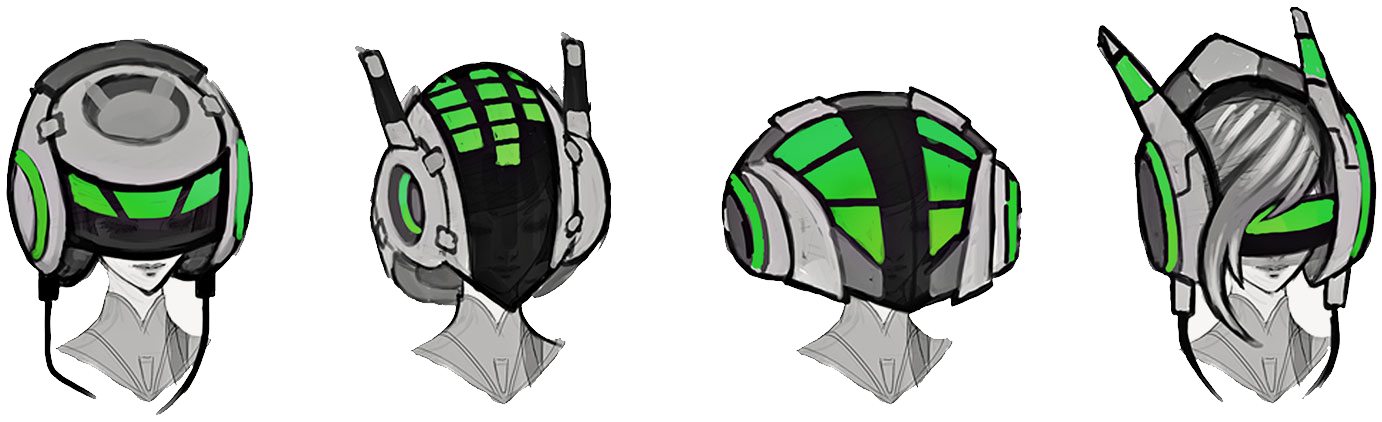
\includegraphics[width=0.85\textwidth]{obrazky-figures/ch2/concept_art.png}
	\caption{Concept art postavy ze hry League of Legends~\cite{artLOLvol1}.}
	\label{fig:concept_art_lol}
\end{figure}

\subsection*{Před-produkce}
Tato fáze přebírá odpovědi z plánování a rozšíří je o důležité detaily. Odehrává se při ní mnoho kolaborací mezi různými týmy (spisovatelé, programátoři, umělci, designeři, ...), aby se vyhovělo co nejvíce požadavkům a zabránilo se pozdějším komplikacím\,--\,programátoři například spisovatelům přiblíží technologické překážky platformy, které není možné překročit, či umělci a designeři navrhnou konzistentní barevné palety.~\cite{g2_game_development}.

Výsledkem před-produkce je dokument o herním designu (\textit{Game Design Document}, neboli GDD) a dokument technického návrhu a mohou zde být navrhovány první prototypy~\cite{novak2011game}. GDD je \uv{živý} dokument a vyvíjí se postupně po celou tvorbu hry\,--\,nalezneme tam detailní popis věcí jako například myšlenku hry, její žánr, celkový příběh, strategii monetizace, informace o postavách, základní herní mechaniky, design úrovní a světa, skici a \textit{concept arty}, neboli návrhy objektů/prostředí/postav~\cite{CG_Spectrum_GAMEDEVELOPMENT} (ukázka concept artu je na obrázku~\ref{fig:concept_art_lol}).

\subsection*{Produkce}
Nejdelší, nejdražší, nejnáročnější a nejdůležitější část vývoje~\cite{g2_game_development}, jejíž výsledkem je hotová hra. 

V této fázi je postupně vytvářen finální produkt. Jsou vymodelovány a animovány objekty, jako jsou postavy či prostředí, které jsou dále naprogramovány, čímž se přidají herní mechaniky a objekty jsou přivedeny k životu~\cite{GameMaker_development}. Tomu napomáhají i zvukoví designeři~a~dabéři, kteří se starají o audio stránku hry.

Při produkci nejsou neobvyklé změny, kde je nutné smazat i celé segmenty hry~\cite{g2_game_development}. Často se stává, že je nutné změnit nějaké navržené či již vytvořené části, ať už je to kvůli nutnosti zmenšit pracovní zátěž vývojářského týmu, či kvůli zjištění, že neimplementovaný objekt do hry nesedí, či nefunguje podle původních představ\,--\,jako například postava \uv{Boatman} ze hry Spyro the Dragon (viz obrázek~\ref{fig:spyro_cut}), která byla změněna na postavu \uv{Ballonist}, nejspíše aby dávalo větší smysl cestování na ostrov v oblacích~\cite{GameMaker_development}.

\begin{figure}[hb]
    \vspace{0.5cm}
    \centering
    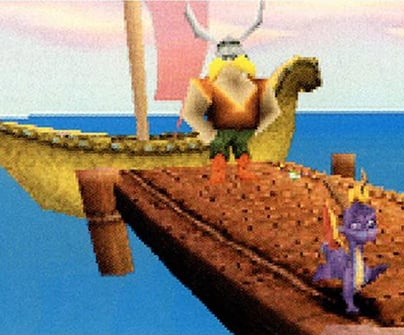
\includegraphics[width=0.5\textwidth]{obrazky-figures/ch2/Spyro-Boatman.png}\hspace{0.1cm}
    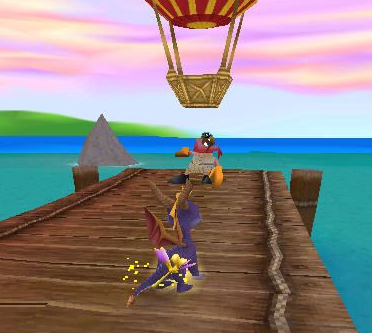
\includegraphics[width=0.46\textwidth]{obrazky-figures/ch2/Spyro-Ballonist.png}
    \caption{Postava Boatman (vlevo) ze hry Spyro the Dragon, který byl ve finální hře změněn na postavu Ballonist (vpravo)~\cite{GameMaker_development}.}
    \label{fig:spyro_cut}
\end{figure}

\subsection*{Testování}
Další důležitou fází je testování. V této fázi je důležité protestovat všechny možné problémy hry, které by mohli kazit zážitek ze hry.

Testy se dají rozdělit na 2 základní typy\,--\,testy technické stability a testování takzvaného \uv{fun factoru} hry, což je průzkum hratelnosti hry, její zábavnosti, poutavosti, a nebo zda není moc těžká, či lehká~\cite{GameMaker_development}. Testy technického faktoru zkoumají, zda se hra správně renderuje, neseká se, dále testeři vyhledávají různé bugy/chyby (např. zda opravdu nejde projít zdmi, nebo jestli se postavička projde místy, kterými by měla v pořádku projít), zda všechny funkce a postavy fungují tak jak mají a další podobné věci~\cite{g2_game_development}.

\subsection*{Před-publikace}
Fáze před publikací je marketingová. Je to období kdy se k veřejnosti dostanou trailery, teasery a demo verze hry~~\cite{GameMaker_development}. Díky tomu může hra získat větší fanouškovskou základnu a~vydavateli může dostat první zpětnou vazbu od veřejnosti.

\subsection*{Publikace}
Vypuštění a distribuce plné verze hry publiku.

Do spuštění hry musí být opraveno co nejvíce (při nejlepším všechny) chyb, proto často studia přichází s hierarchií chyb, které jsou potřeba opravit, od těch nejproblémovějších, které například rozbíjí hru, tak že často padá, až po ty nejdrobnější~\cite{g2_game_development}.

\subsection*{Post-produkce}
V této etapě již hru vlastní a hraje veřejnost, často je ale vydáno zdarma několik dalších verzí hry (zvané \textit{patch}), které ji technicky vylepšují, vyvažují a často i opravují chyby~\cite{novak2011game}, na které se nedostalo při produkci, či které byly nově objeveny hráči. 

Také zde mohou přibýt \textit{updaty}, které do hry přidávají nový obsah (například události (\textit{eventy}), nové postavy/místa, atd.)~\cite{g2_game_development}. Nový obsah přidávají také rozšíření neboli DLC, které jsou ale často oproti updatům placené, nabízí více obsahu, a pro jejich spuštění vyžadují vlastní software (občas v kombinací s originální hrou) na spuštění~\cite{novak2011game}. Nový obsah udržuje hru relevantní~\cite{GameMaker_development}.

\subsection*{Milníky verzí vývoje her}
V průběhu vývoje videohra projde několika různými verzemi, které se od sebe liší jejich technickými vlastnostmi, kniha Game Development Essentials: An Introduction~\cite{novak2011game} uvádí nejdůležitější 3 z nich uvedené níže.
\begin{itemize}
    \item Alfa\,--\,v této fázi je již hra hratelná od začátku k cíli a je označována jako \textit{\uv{feature complete}}~\cite{CG_Spectrum_GAMEDEVELOPMENT}, což znamená že všechny hlavní vlastnosti jsou již implementované, nemusí zde být ale vše kompletně zoptimalizované. Měla by to být první verze testovaná lidmi mimo vývojářský tým.
    \item Beta\,--\,hra již v sobě má integrovaný všechen obsah, zaměření už je jen na opravě chyb a stabilizování projektu.
    \item Gold\,--\,finální dodělaná hra, která je připravena na publikaci.
\end{itemize}

%--------------------------
% Začátek videoher
\section{Začátek videoher}
První počítačové hry vznikaly kolem 50. let 20. století na vojenských základnách a univerzitách a jejich sálových počítačích~\cite{novak2011game}\,--\,těmito videohrami byla například OXO (1952), Tennis for Two (1958), ale do nepopulárnějších videoher (vytvořených v té době) se počítá hlavně hra vytvořena MIT studentem Stevem Russellem Spacewar!~\cite{bellis2019spacewar}, jenž je vidět na obrázku~\ref{fig:spacewar}. 


Nápad této hry byl následně, na začátku 70. let, přebrán Nolanem Bushnellem (zakladatelem Atari), který z ní vytvořil první komerční arkádovou hru (a tedy volně přístupnou veřejnosti) pod jménem \uv{Computer Space}, která byla velmi úspěšná~\cite{video_games_history}. To spustilo vývoj dalších velmi úspěšných arkádových videoher, oproti dnešním hrám převážně dovednostích, jako například \uv{Pong}, či \uv{Space Invaders} a \uv{Asteroids}, což byly první hry umožňující hráčům ukládat své skóre, dále například Galaxian, Pac-Man, Donkey Kong a Tron~\cite{novak2011game}.

Ve stejnou dobu začal i vývoj konzolových her, tedy možností hrát hry v pohodlí domova. Příklady firem, jejich konzolí a her (či herních sérií), které vznikli kolem této doby a zasloužili se o rozvoj konzolových/počítačových her, jako je známe dnes, jsou vypsány v~následujícím odstavci.
\begin{itemize}
    \item Atari\,--\,roku 1976 vydali jednu z prvních konzolí Atari VCS/2600, která odstartovala velkoprodej domácích konzolí~\cite{novak2011game}. Tato konzole přišla s mnoha, pro svojí dobu, ikonickými hrami, které byly často předělané tituly známe z arkád, jako je například Pac-Man série, Space Invaders, Asteroids, Q*bert, Pole Position či Frogger~\cite{Atari_games}.
    \item Nintendo\,--\,jejich první konzole, NES, byla vydána roku 1985. Vyšlo na ni mnoho dodnes populárních herních titulů, jako je například The~Legend of~Zelda, Super Mario Bros, Final Fantasy, Dragon Quest nebo Tetris~\cite{NES_GAMES}.
    \item Sega\,--\,jejíž první konzolí byla SG-1000 z roku 1983 s nejpopulárnější vydanou sérií Sonic the~Hedgehog~\cite{SegaRetro_2023}.
\end{itemize}

S příchodem personálních počítačů do domácností se zvýšil zájem o hry, mnoho původně pouze univerzitních her, bylo adaptováno do personálních počítačů, což způsobilo úpadek placených arkádových her~\cite{novak2011game}. 

V dnešní době jsou možnosti pro hraní videoher ještě rozšířenější, od možnosti hrát na telefonech, vyvinutějších ručních konzolích, či pomocí virtuální reality.

\begin{figure}[H]
    \centering
	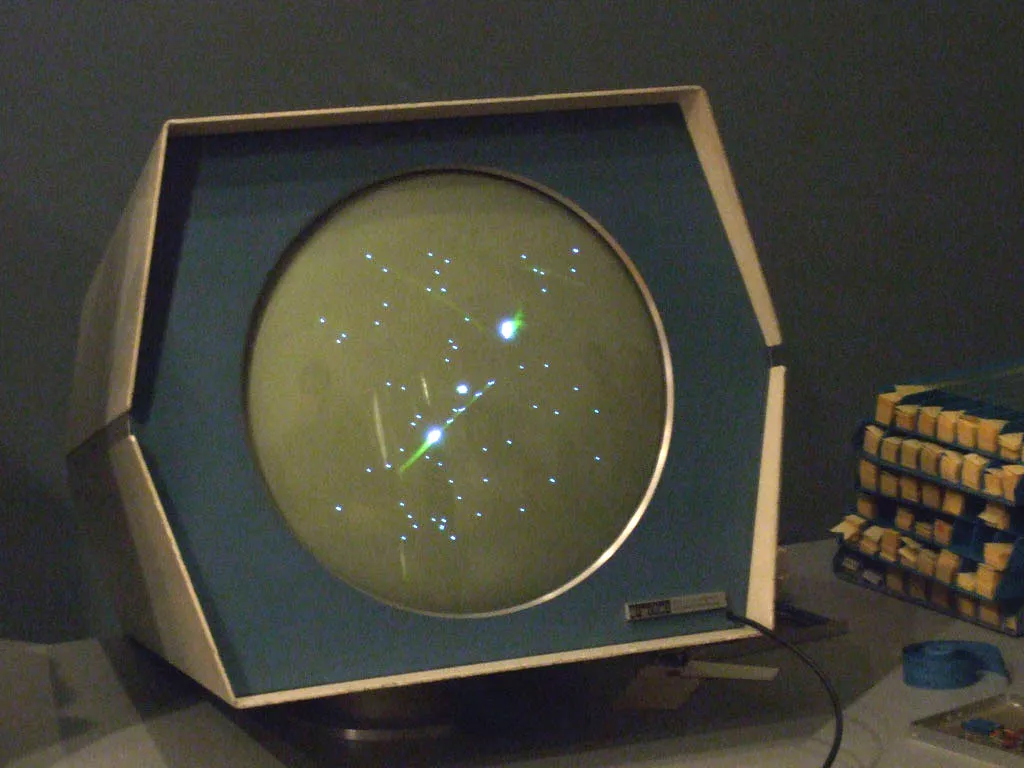
\includegraphics[width=0.53\textwidth]{obrazky-figures/ch2/Spacewar.png}
	\caption{Ukázka hry Spacewar~\cite{bellis2019spacewar}.}
	\label{fig:spacewar}
\end{figure}

%--------------------------
% Labyrintové hry
\section{Labyrintové videohry}
Dle Akademického slovníku současné češtiny~\cite{AkademickySlovnik-Bludiste} je bludiště, neboli labyrint, definováno jako \uv{místo, kde se bloudí} a \uv{složitý, neuspořádaný systém}. Bludiště jsou multikurzální, je to tedy spleť cest, chodeb a prostor, kde se snadno zabloudí a jsou definovaná slepými konci a~větvícími chodbami, kvůli kterým je procházející nucen se rozhodovat.

Andrew Rollings a Ernest Adams definují bludiště ve hrách jako prostředí, kde každé místo vypadá stejně, nebo velmi podobně a hráč musí zjistit, jak jsou místa propojená, často jejím procházením, aby našel cestu ven~\cite{rollings2003andrew}. Tyto hry jsou často doplněné o i nějaké výzvy než pouze procházení bludištěm, kterými, dle stejných autorů~\cite{rollings2003andrew}, může být například hledání klíče k otevření zamknutích dveří, sbírání věcí (např. pro zvýšení skóre), řešení hádanek, paměťových testů, luštění kryptických zpráv, atd.

V 80. letech 20. století měly hry s tématem bludiště největší rozmach, hlavně kvůli rozšíření domácích konzolí (např. Atari 2600), a díky jejich množství a rozmanitosti je lze rozdělit na 4 typy~\cite{DoYouMaze}:
\begin{itemize}
    \item bludiště s pohledem z vrchu\,--\,při hraní je vidět celé (či skoro celé) bludiště z vrchu (Mouse in the Maze, Bomberman),
    \item bludiště z prvního pohledu\,--\,stejný pohled na hru, jako herní postavička (Maze/Maze War, Capture the Flag),
    \item pronásledování bludištěm\,--\,hráč je pronásledován, či může pronásledovat nepřátele; tento typ je propojen s různými styly pohledu na bludiště (Pac-Man, Rally-X, Lady Bug),
    \item bludiště s obsazováním políček mřížky\,--\,hráč při průchodu bludištěm musí zabrat co nejvíce políček (Amidar).
\end{itemize}

\noindent Dále v textu se nachází příklady různých významných labyrintových her vytvořených v~průběhu historie.

\begin{figure}[H]
	\centering
	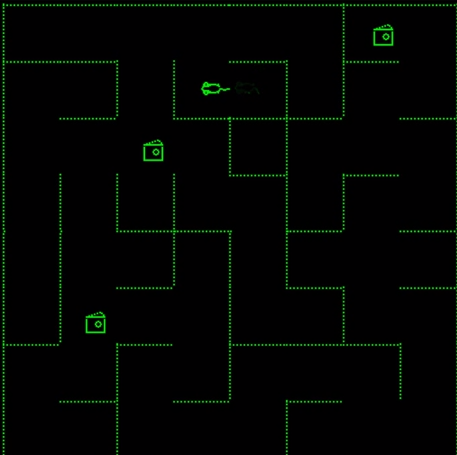
\includegraphics[width=0.5\textwidth]{obrazky-figures/ch2/MOUSE.png}
	\caption{Ukázka ze hry Mouse in the Maze.~\cite{Videogamehistorian}}
	\label{fig:mouse}
\end{figure}

\subsection*{Mouse in the Maze}
První labyrintovou hrou byla hra s názvem \textit{MOUSE}, nebo také \textit{Mouse in the Maze}, naprogramovaná roku 1959  Douglasem T. Rossem a John E. Wardem na sálovém počítači TX-0~\cite{TheOriginOfSpacewar}. 

Hráč dostal 8x8 mřížku a následně mohl světelným perem odmazat zdi a přidat sýr(y) (či v upravené verzi martini) a následně sledovat myš procházející bludiště, kde si pamatovala již prošlé cesty, a hledající sýr, který musela najít než se vyčerpala~\cite{Videogamehistorian}. Ukázka ze hry je zobrazena na obrázku~\ref{fig:mouse}, ze kterého je vidět, že hra je bludiště s pohledem z vrchu.

\subsection*{Maze/Maze War}
3D labyrintová pronásledující střílecí hra z roku 1974 vyvinutá studenty MIT~\cite{Maze_War}. Byla to průlomová hra, nabízející nejen iluzi 3D grafiky, ale i podporou hraní až pro 8 hráčů, či nehráčské boty a byla nejspíše jednou z prvních, či možná i první střílecí hrou~\cite{virtual_worlds}. Později byla hra díky využití TCP/IP protokolu, díky kterému hráči mohli hrát mezi sebou po internetu, průkopníkem i v online hrách~\cite{Maze_War}.

Úkolem hráčů, hrající jako avatar oční bulvy, bylo projít bludiště (kde mohli chodit pouze dozadu, dopředu a otáčet se o 90° vpravo, či vlevo), najít nepřátele a střelit je, čímž sbírali skóre~\cite{Maze_War}.

\subsection*{Pac-Man}
Japonská arkádová hra od společnosti Namco (dnes Bandai Namco Entertainment) vyšla původně v roce 1980 pod jménem Puck-Man (kvůli jeho tvaru puku, jméno ale bylo pro USA změněno, kvůli strachu z vandalů~\cite{kent2010ultimate}) a po svém vydání v USA se z ní stal okamžitý hit, neboť se v jednom roce prodalo více než 100 000 arkádových automatů s touto hrou~\cite{PACMAN}. Hitem byly i další hry z rychle rostoucí série Pac-Man. Roku 1981 vyšla Ms. PAC-MAN, jenž získala několik nových herních prvků, jako například více bludišť (oproti pouze 1, které nabízel originál) či náhodnější nepřátele\,--\,po svém vydání prodala i tato hra v USA více než 100 000 automatů, což žádná jiná hra v USA nedokázala~\cite{kent2010ultimate}.

\begin{figure}[hb]
	\centering
	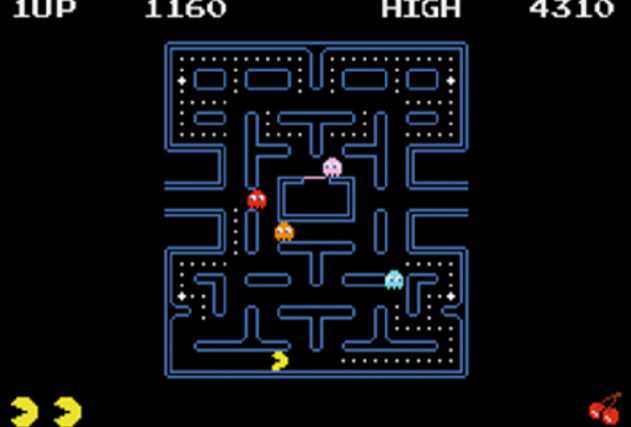
\includegraphics[width=0.7\textwidth]{obrazky-figures/ch2/pacman.png}
	\caption{Ukázka ze hry Pac-Man.~\cite{von2007space}}
	\label{fig:pacman}
\end{figure}

Pac-Man je hra založena na principu pronásledování hráče nepřáteli bludištěm~\cite{kent2010ultimate}, jak je vidět na obrázku~\ref{fig:pacman}. Hráč má za úkol projít bludiště a sebrat všechny tečky na zemi, čímž se dostane do další úrovně. Při tom ho ale pronásledují 4 duchové, kteří pokud ho chytí tak Pac-Man ztratí jeden ze 3 životů (když ztratí všechny, hra je prohraná). Hráč nadále může získat bonusové body díky sebranému ovoci, nebo pomocí bonusů, čímž se na omezenou dobu může nazpátek Pac-Man pojídat duchy.

\subsection*{Bomberman/Dyna Blaster}
Další labyrintová hra od japonských vývojářů, která je podobně jako Pac-Man, populární a vydávaná dodnes je Bomberman, v Evropě známý pod názvem Dyna Blaster, vydaný v roce 1983 (1985 na Nintendo konzole), kterého se prodalo za několik prvních let skoro milion kopií~\cite{Bomberman}. 
Mapa hry je jednoduchý obdélník s několika systematicky rozdělenými nerozbitnými zdmi, mezi nimiž se nachází volná místa a rozbitné zdi. Hráčův úkol je zničit všechny nepřátele pomocí pokládání bomb, které po určitém čase vybouchnou v křížovém tvaru, čímž zlikvidují nepřátele a rozbijí zdi v jeho výbušné oblasti, a také odejít dveřmi, které jsou schované za jednou ze zničitelných zdí~\cite{Bomberman}. 

%--------------------------
% Herní engine
\section{Herní engine}\label{chap:Herní engine}
Herní engine (také game engine) je softwarový framework využívaný pro tvorbu a vývoj (nejen) videoher. Nabízí mnoho nástrojů pro zjednodušení tvůrčího procesu, jako jsou například podpůrné programy, knihovny, a některé poskytují i speciální programovací jazyky vytvořené specificky pro programovaní her v daném engine~\cite{Valencia-Garcia_2016}. V následující části textu jsou popsány a uvedeny některé příklady z nejpopulárnějších herních enginů (viz obrázek~\ref{fig:most_popular_game_engines}).
\begin{figure}[H]
    \vspace{0.5cm}
	\centering
	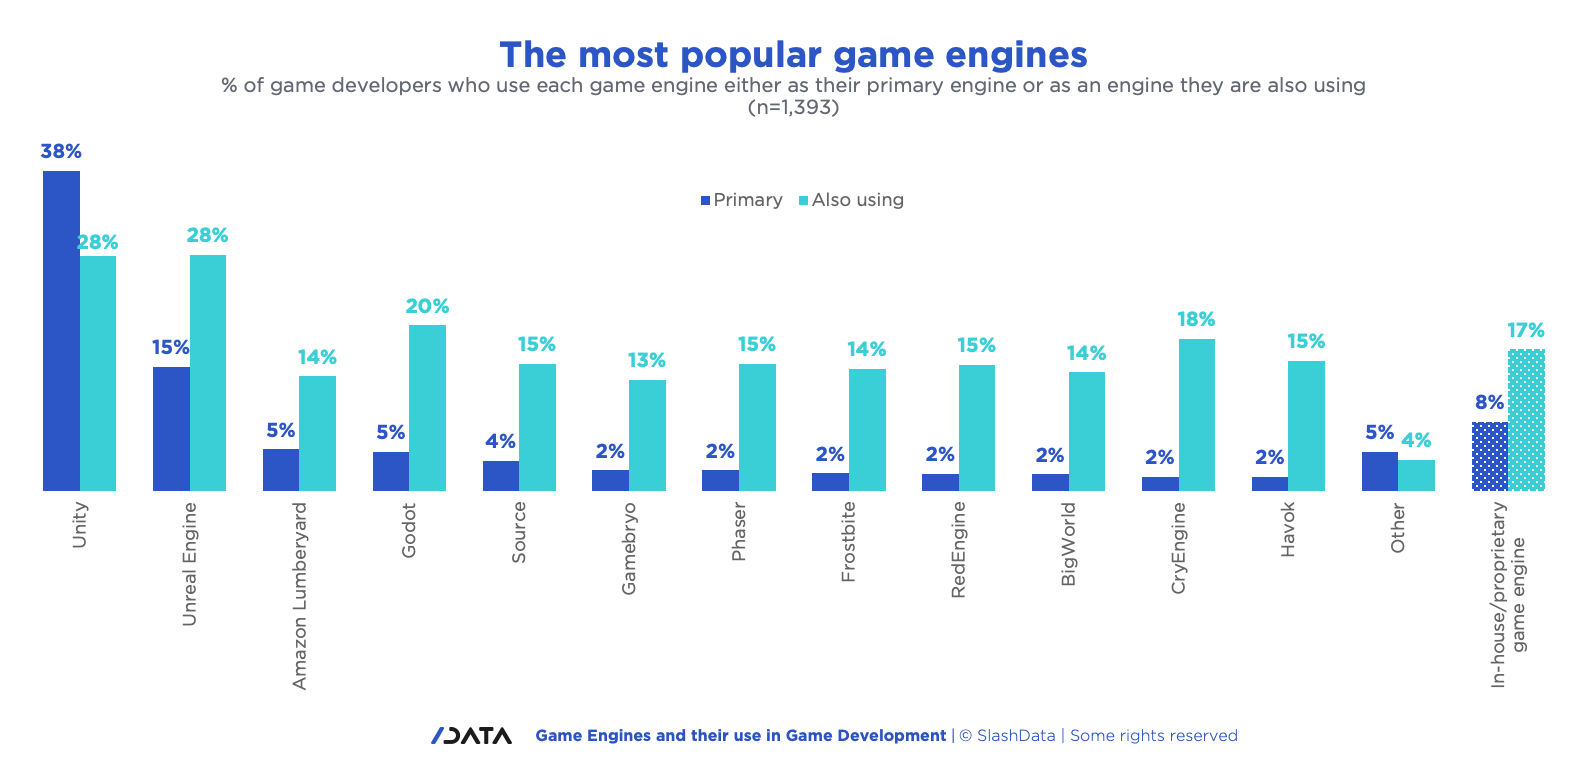
\includegraphics[width=\textwidth]{obrazky-figures/ch2/most_popular_game_engines.png}
	\caption{Výzkum SlashData z roku 2021 o nejpoužívanějších herních enginů.~\cite{SlashData_game-engines}}
	\label{fig:most_popular_game_engines}
\end{figure}

\subsection*{Unity}
Unity je multiplatformní game engine od společnosti Unity Technologies. Dle oficiálních webových stránek aktuálně podporuje více než 20 platforem (např. Windows, macOS, Linux, Android, PlayStation 5, Nintendo Switch,~\ldots)~\cite{unity_website}, nejen díky čemuž je jedním z~nejpoužívanějších softwarů na tvoření her~\cite{arnia_unity}. Poskytuje bezplatnou verzi (pro soukromé užití, nebo pokud výdělek hry za rok nepřesahuje 100 000\$) i placenou verzi \uv{Unity Pro}. 

Pro implementaci her, ať už 2D, 3D či VR (hry pro virtuální realitu), nabízí možnost vizuálního/grafického editoru a skriptů v C\#. Základní herní entita je \verb|GameObject|, které je množné přiřazovat různé vlastnosti, herní mechaniky, grafiku atd. a to již předefinované, či naprogramované uživatelem pomocí skriptů. Různé \verb|GameObjects| můžou být součástí \verb|Scene| z čehož je následně konstruován finální produkt~\cite{hocking2015unity}.

Unity je hojně využívána na vývoj AAA (také Triple-A hry neboli produkt od distributora, pro jehož vývoj byl k dispozici bohatý rozpočet) her, například: Marvel Snap, Apex Legends, ale i indie (takzvaně od nezávislých tvůrců = independent creator), například: Cult of the Lamb, Among Us, Slime Rancher, Cuphead~\cite{unity_website}.

\subsection*{Unreal Engine}
Unreal Engine je série herních engine, s nejnovější verzí Unreal Engine 5 z roku 2022, od společnosti Epic Games. První verze byla vytvořena pro tvorbu Unreal, 3D střílečky z pohledu první osoby, a byla velmi populární, jelikož díky UnrealScriptu (založeném na C++) mohli uživatele jednoduše původní hru modifikovat~\cite{sanders2016introduction}. Novější verze využívají klasické C++. Podobně jako Unity, nabízí bezplatnou i placenou verzi. Je také multiplatformní, ale podporuje menší škálu platforem než Unity\,--\,základní (Windows, Linux, PlayStation, Nintendo Switch, Xbox), ale podporuje~\cite{unreal_engine}.

V porovnání s dalšími zástupci herních engine je hodnocen jako jeden ze složitějších. Díky své komplikovanější stavbě a strmé křivce učení práce s Unreal Engine je doporučován spíše na větší, komplikovanější projekty, než například na mobilní hry (i přestože podporuje vývoj her na Android)~\cite{Kevuru_Games_Unreal-Unity}. Unreal Engine 5 je zaměřený hlavně na 3D vývoj a proto přišel s~mnoha funkcemi pro vylepšení vykreslování a práci s trojdimenzionálními objekty - jsou to Nanite (vizuální geometrický systém), Lumen (vylepšená práce se světlem) a MetaSounds (managment audia)~\cite{UnrealEngine5}.

Hrami, které byly vytvořeny za pomocí Unreal Engine je například Minecraft Dungeons, Final Fantasy VII Remake, Fortnite (ukázka na obrázku~\ref{fig:fortnite-unreal_engine}) nebo Stray~\cite{unreal_engine}.

\begin{figure}[H]
	\centering
	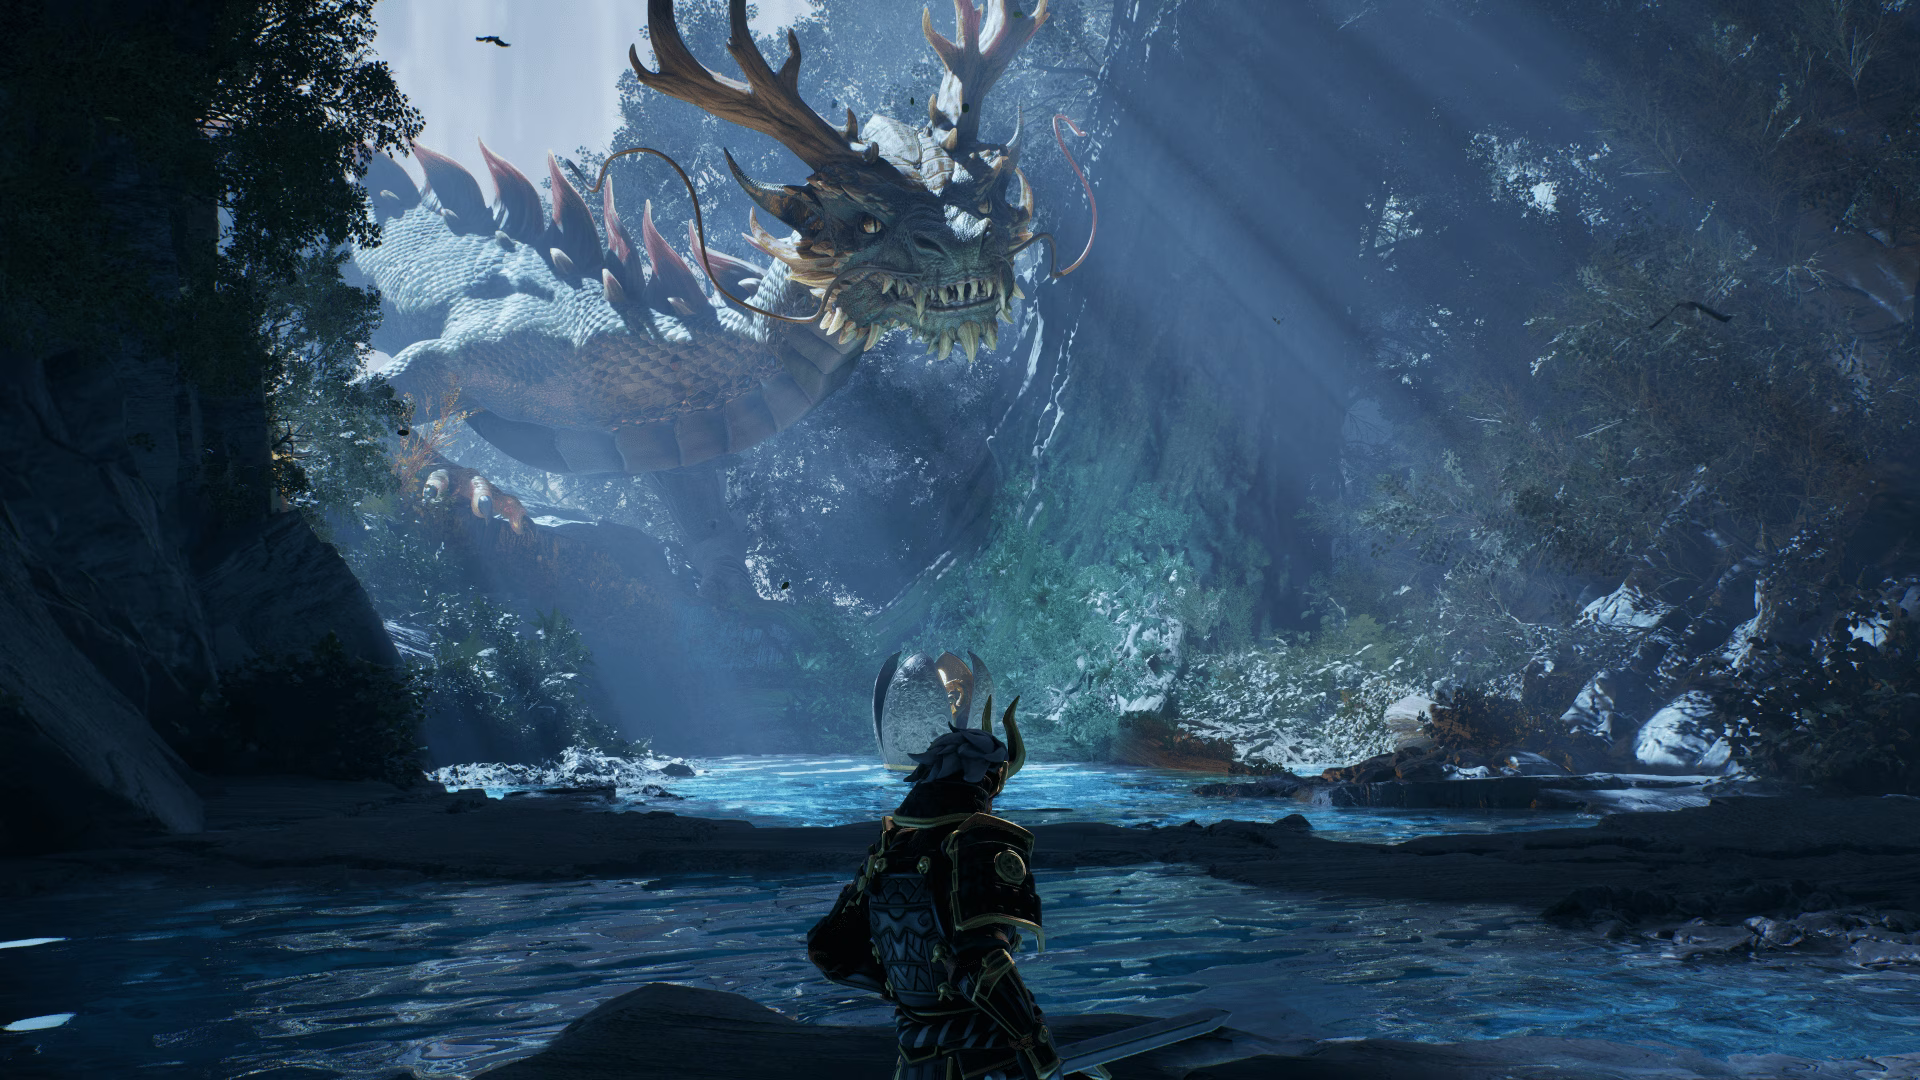
\includegraphics[width=0.66\textwidth]{obrazky-figures/ch2/fortnite.png}
	\caption{Ukázka ze hry Fortnite vytvořená pomocí Unreal Engine 5.~\cite{unreal_engine}}
	\label{fig:fortnite-unreal_engine}
\end{figure}

\subsection*{Godot}
Godot (s nejnovější verzí 4.2.1) je další software pro tvorbu 3D a 2D her. Na rozdíl od Unity a Unreal Engine je od verze 3.0 kompletně zdarma, svobodný a otevřený (open-source)\footnote{\url{https://github.com/godotengine/godot}}. Kvůli tomu má ale Godot oproti jiným zmíněným herním engine omezené oficiální možnosti platforem, jelikož jsou konzole (PlayStation, Xbox) uzavřené ekosystémy a Godot nimi není licencovaný~\cite{Godot_Engine_consoles}. Stále ale podporuje škálu platforem, příkladem desktopové (Windows, Linux, macOS), webové (HTML5), mobilní (Android, iOS) a virtuální realita (Oculus Rift/Quest, HTC Vive).

Základní stavební blok pro vytváření projektu v Godot je \verb|Node| (objekt reprezentující specializovaný prvek)\,--\,tyto objekty lze následně propojovat do \verb|Scene|, jak je vidět na obrázku~\ref{fig:godot_view}, což jsou stromy závislostí tvořící finální produkt~\cite{bradfield2018godot}. K těmto \verb|Nodes| lze přiřazovat skripty v jazycích GDScript (dynamicky typovaný jazyk syntaxí podobný Pythonu), C\# a C++\cite{GameEngineWizardry}. Godot se oproti předešlým zmíněným softwarům zaměřuje na 2D, pro které nabízí optimalizovaný přístup zdůrazňující jednoduchost a efektivitu (např. \verb|TileMap|, pro tvoření map, či \verb|Sprite2D| s vlastnostmi pro funkci 2D postav)~\cite{Godot_Engine}.

V Godotu byly vytvořeny například hry Brotato, Hive Time, Tail Quest a aplikace Dungeoncraft a Material Maker~\cite{Godot_Engine}.
\begin{figure}[H]
	\centering
	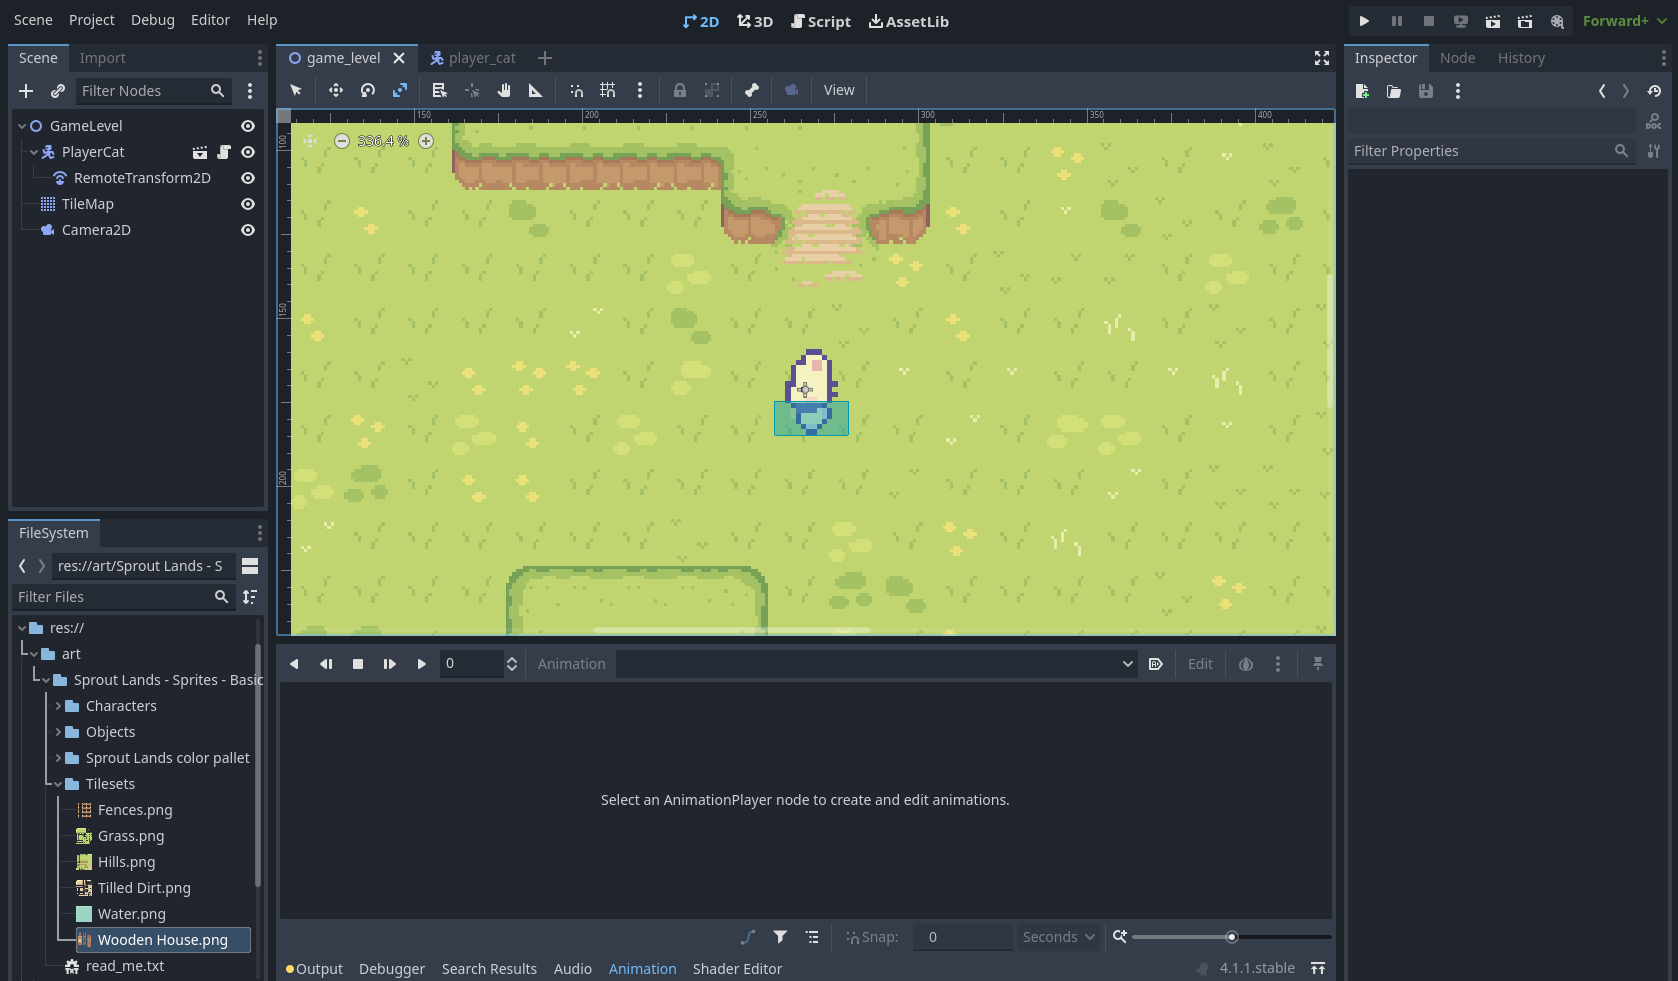
\includegraphics[width=0.8\textwidth]{obrazky-figures/ch2/godot_view.png}
	\caption{Grafické rozhraní pro zobrazení Scene v Godot verzi 4.2.}
	\label{fig:godot_view}
\end{figure}

%--------------------------
% Celulární automaty
\section{Celulární automaty}
Celulární automat (nadále označován také zkratkou CA) je dynamický systém a diskrétní model prostorového systému využívaný na modelování fyzikálních či biologických simulací. Prostorový systém vyjadřuje prostorovou dekompozici systému\,--\,zkoumaný systém je rozdělen na malé části s definovaných chováním~\cite{ims}.

\subsection*{Základní definice }
Celulární automat je čtveřice ${(\alpha^{n}, S, N, f)}$, kterou lze dle Stanfordské encyklopedie filozofie~\cite{sep-cellular-automata}, definovat následovně:
\begin{itemize}
    \item ${ \alpha^{n} }$ (\textit{Lattice}) je diskrétní n-dimenzionální mřížka buněk (${ n >= 1 }$)\,--\,tyto buňky jsou identické (některé mohou být speciální\,--\,např. modelují pevné hranice), 
    \item ${ S }$ je konečná množina stavů, které mohou buňky nabývat\,--\,v každém diskrétním časovém kroku může každá buňka nabýt pouze a jenom 1 stavu, 
    \item ${ N }$ je konečná množina sousedících buněk (okolí, které může, či nemusí obsahovat i~buňku samotnou) pro každou buňku, na kterém záleží její vývoj, ${ N \subseteq \alpha }$,
    \item ${ f }$ je konečná množina pravidel pro přechod mezi stavy\,--\,v každém časovém kroku každá buňka aktualizuje svůj aktuální stav podle deterministické přechodové funkce $\phi : \Sigma^n \rightarrow \Sigma$, která mapuje okolí. Často (i když ne nutně) se počítá, že aktualizace synchronní a bere jako vstup okolí v čase $t$ sousední stavy v bezprostředně předchozím časovém kroku $t-1$.
\end{itemize}
Příkladem zápisu definice celulárního automatu Game of Life (vysvětlený níže) lze zapsat jako:
\begin{equation*}
\begin{split}
    & \left( \alpha^{2}, \right. \\
    & \left. \{0, 1\}, \right. \\
    & \left. N(c_i) = \{ c_{i-1,j-1}, c_{i-1,j}, c_{i-1,j+1}, c_{i,j-1}, c_{i,j}, c_{i,j+1}, c_{i+1,j-1}, c_{i+1,j}, c_{i+1,j+1} \}, \right. \\
    & \left. \{B3/S23\} \right)
\end{split}
\end{equation*}

Vlastnosti CA je možné popsat také pomocí řetězců pravidel (anglicky \textit{rulestring}). V~následujícím textu jsou uvedeny 2 příklady přebrané ze stránky LifeWiki~\cite{LifeWiki} pro 2 stavové CA. Těmito stavy jsou 1 = živá buňka a 0 = mrtvá buňka. 
\begin{itemize}
    \item Birth/Survival notace\,--\,Nejpoužívanější notace, která je zapisována pomocí \verb|B{list}| \verb|/S{list}|. Notace je vyjadřována 2 seznamy. V prvním (B) je zapsán počet živých sousedů potřebný pro vznik nové živé buňky, neboli oživení. Druhý seznam určuje kolik živých sousedů musí buňka mít, aby přežila do dalšího kroku. Game of Life by touto notací byla zapsána B3/S23.
    \item S/B notace\,--\,Dříve často používaná, dnes spíše nahrazena Birth/Survival notací. Podobně jako ona je zapisována pomocí 2 seznamů \verb|{list}|\verb|/{list}|. Jeden označuje počet živých sousedů potřebných pro přežití živé buňky a druhý počet živých sousedů potřebných pro oživení mrtvé buňky. Tedy opak Birth/Survival listu. Game of Life je zapsána jako 23/3.
\end{itemize}

Typ okolí závisí na tvaru buněk (čtverec, hexagon,~\ldots) a také typu prostoru (1D, 2D,~\ldots)~\cite{ims}. Dvě nejpoužívanější okolí jsou Moorovo a von Neumannovo s různými variacemi~\cite{sloot2004cellular}, jak je vidět na obrázku~\ref{fig:2D-okoli}.
\begin{figure}[H]
    \centering
    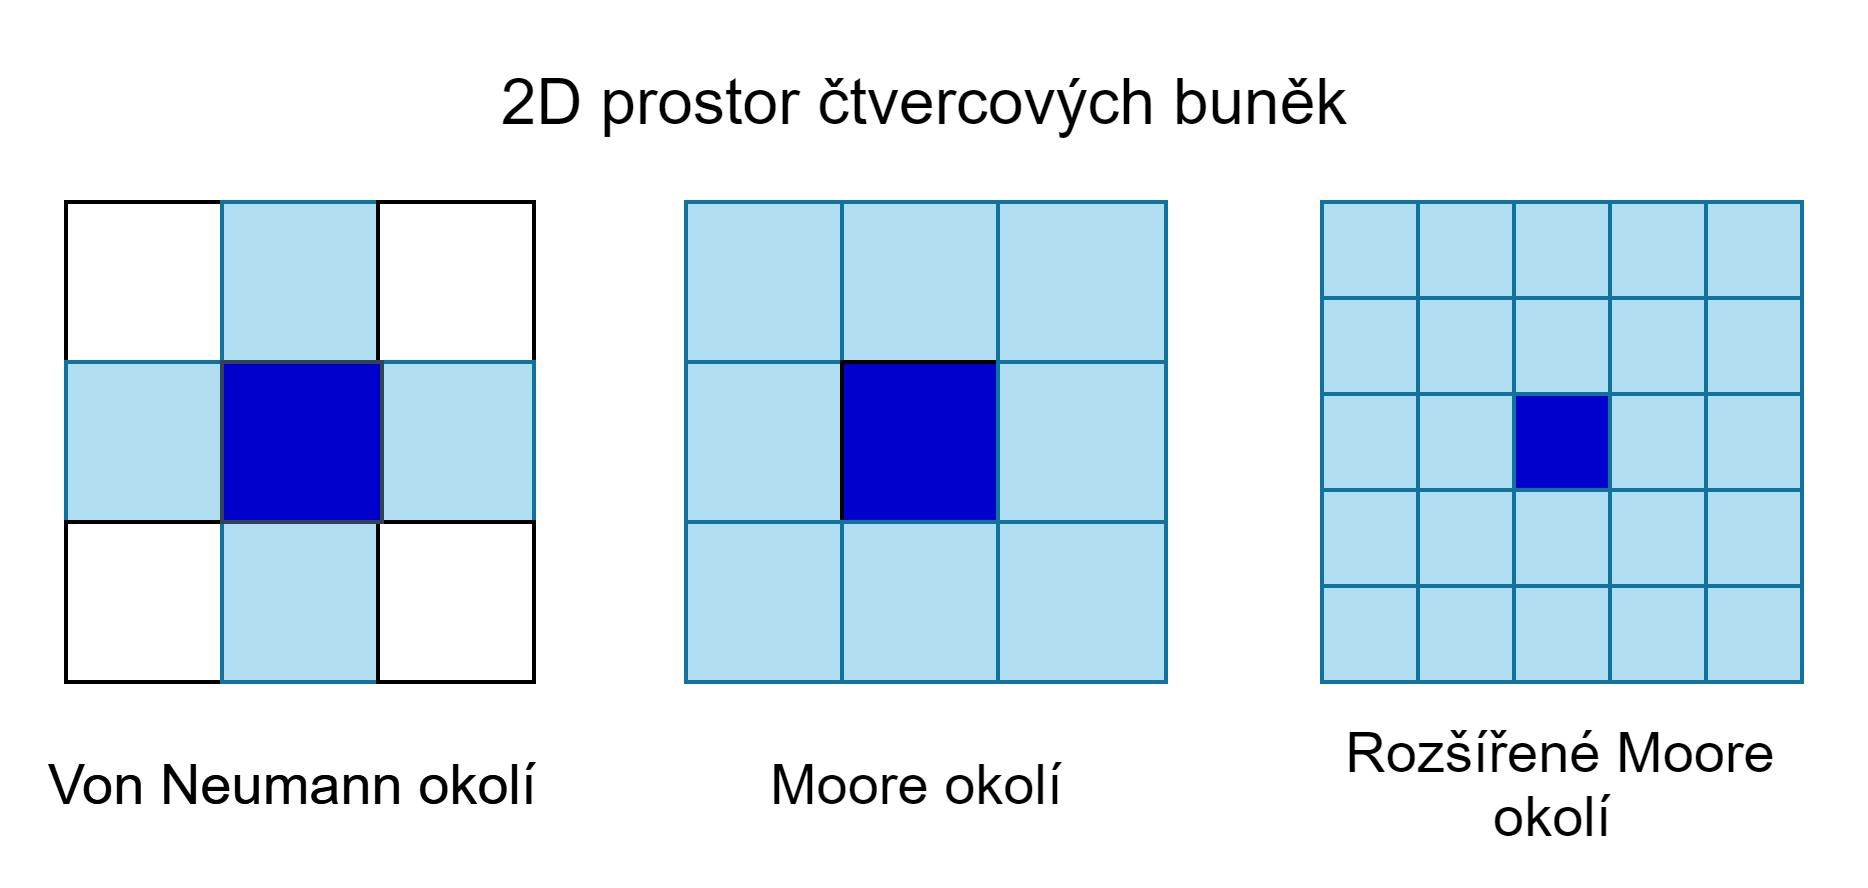
\includegraphics[width=0.65\textwidth]{obrazky-figures/ch2/2D-okoli.png}\hspace{0.5cm}
    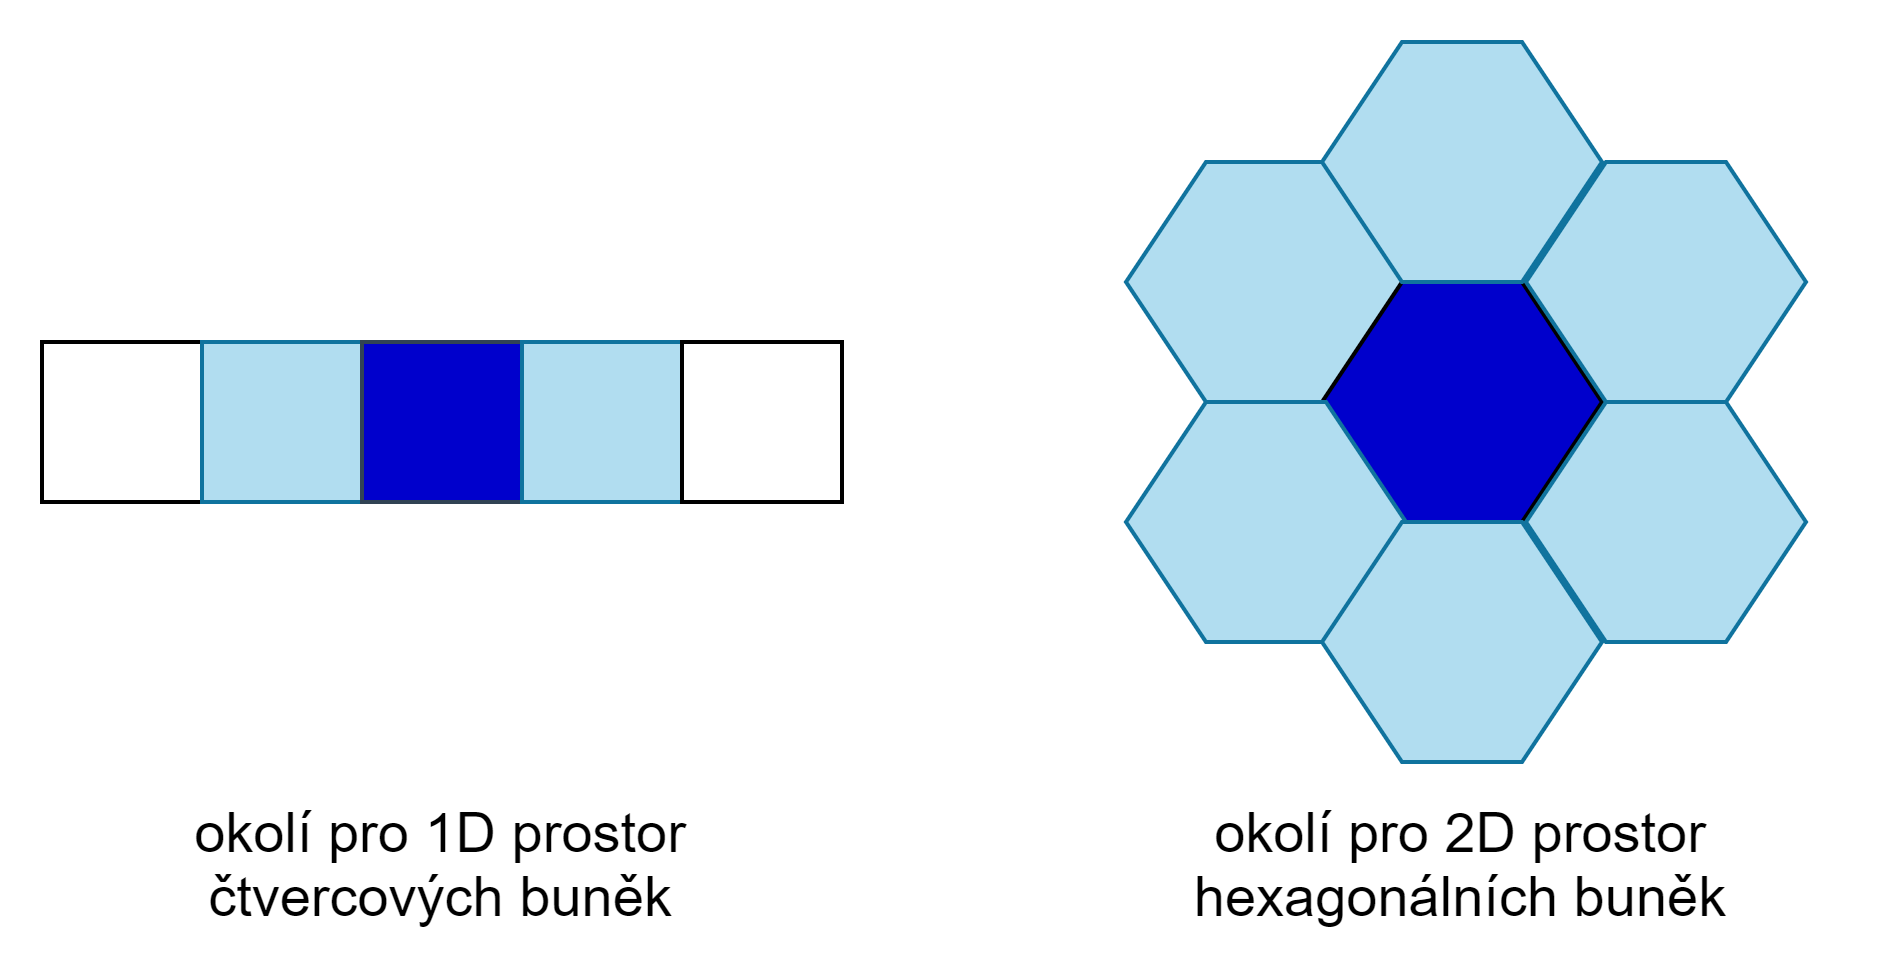
\includegraphics[width=0.65\textwidth]{obrazky-figures/ch2/jina-okoli.png}
    \caption{Příklady okolí (tmavě modrá = zkoumaná buňka, světle modrá = okolí).}
    \label{fig:2D-okoli}
\end{figure}

Jak je již popsáno u formálního popisu, pravidla určují následující stav buňky v čase, který je závislý pouze na jejím aktuálním stavu a stavu jejího okolí, a to pro všechny možnosti vstupu. Pomocí funkce stavu buňky ${s(t)}$ a jejího okolí ${N_s(t)}$ lze vyjádřit rovnici~\ref{eq:CA-rule} pravidla~\cite{ims}.
\begin{equation}
s(t + 1) = f(s(t), N_s(t))
\label{eq:CA-rule}
\end{equation}
Některá pravidla mohou mít i vlastnosti udávající typ pravidlu, které definuje~\cite{mechanics-CA}:
\begin{itemize}
    \item \textbf{totalistic} = o výsledku rozhoduje součet hodnot vstupních buněk (např. Game of Life),
    \item \textbf{legal} = z nulového vstupu nemůže samostatně vzniknout nenulový.
\end{itemize}

\subsection*{Klasifikace}
Stephen Wolfram ve své knize \textit{A New Kind of Science}~\cite{wolfram-NewKindOfScience} definoval 4 třídy pro dělní CA, vypsané níže.
\begin{enumerate}
    \item Téměř všechny počáteční vzory CA se po konečném počtu kroků dostanou do 1 stabilního, homogenního stavu. Zmizí jakákoliv náhodnost v počátečním vzoru.
    \item Téměř všechny počáteční vzory CA se vyvinou do periodicky se opakujících (oscilujících) struktur/stavů nebo zůstane stabilně v některém ze stavů.
    \item Deterministický chaos\,--\,téměř všechny počáteční vzory se vyvíjejí pseudonáhodným, nebo chaotických způsobem. Stabilní struktury, které se objeví jsou rychle zničeny okolním hlukem.
    \item Téměř všechny počáteční vzory se vyvíjejí do struktur, které interagují složitým a zajímavým způsobem, s tvorbou místních struktur, které jsou schopny přežít po dlouhou dobu. Konečným výsledkem mohou být stabilní nebo oscilující struktury typu 2 (k~dosažení může být ale potřeba velký počet kroků). Pod tuto třídu patří Game of Life (viz níže).
\end{enumerate}

Některé celulární automaty lze označovat také jako \textbf{reverzibilní}. Ty jsou definované jako systémy, které neztrácí informaci při svém vývoji v čase\,--\,což znamená, že v každém okamžiku lze otočit vývoj času a navrátit se k předchozím stavům~\cite{ims}. Kvůli jejích chaotickému chování nejsou CA 4. třídy nikdy reverzibilní.

\subsection*{Historie a Game of Life}
Za vznikem celulárních automatů stáli ve 40. letech 20. století matematici John von Neumann a~Stanisław Ulam. Ulam studoval růst krystalů pomocí jednoduché mřížky~\cite{pickover2009math} a~von Neumann řešil modely samoreprodukujících se organismů~\cite{history_CA}. Ulam von Neumannovi navrhl využití diskrétního systému~\cite{schiff2011cellular} s buňkami, které se mění po jednotlivých krocích/iteracích. Na základě dalšího výzkumu došli k vyvinutí základů CA a John von Neumann následně na základě myšlenek celulárních automatů sepsal knihu \textit{Theory of Self-Reproducing Automata}, kde detailně, spolu s důkazy o jeho možné existenci, popisuje jeden z prvních konceptů realistických samo-replikujícího systému, \textit{von Neumannův univerzální konstruktor}~\cite{theory_neumann} který funguje jako univerzální kopírka, která by v teorii replikovala sebe sama pomocí surovin z prostředí, ve kterém se nachází. 

Dalším z důležitých matematiků pro vývoj CA byl John Conway, který v roce 1970 vytvořil pravidla pro \textbf{Game of Life}~\cite{history_CA}, celulární automat na 2D mřížce s buňkami nabývajících 2 stavů\,--\,živá, mrtvá, využívající Moorovo okolí o 8 sousedech (viz obrázek~\ref{fig:2D-okoli}). Pravidly jsou~\cite{Game_Of_Life}:
\begin{itemize}
    \item pokud živá buňka sousedí s 2 nebo 3 živými sousedy přežívá do další generace,
    \item neživá buňka, která má přesně 3 živé sousedy oživne,
    \item zbytek buněk do další generace nepřežívá a stává se mrtvými.
\end{itemize}
I přes svoji jednoduchost tento systém nabývá klasifikace 4. třídy, tedy projevuje náhodnost, ale zároveň se v jeho generacích objevují struktury, které vykazují rozmanité vlastnosti a~dodávající systému částečný řád. Jedním z těchto struktur, je takzvaný kluzák (anglicky \textit{glider}), který se postupem iterací pohybuje po mřížce~\cite{Game_Of_Life}. Ilustraci jeho pohybu je možné vidět na obrázku~\ref{fig:game_of_life}.
\begin{figure}[H]
    \centering
    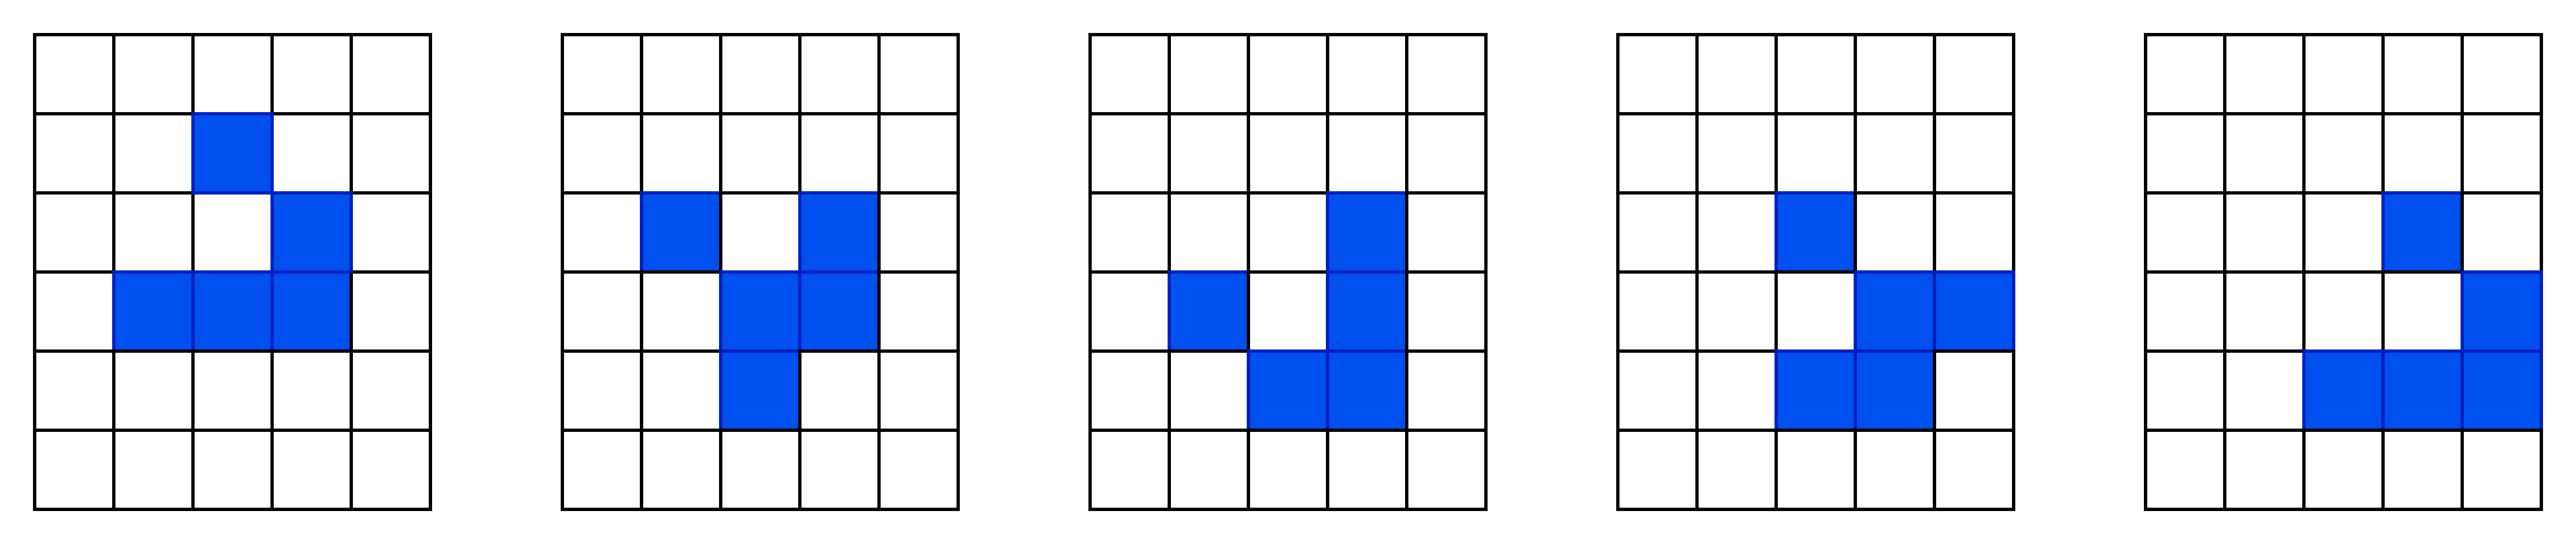
\includegraphics[width=\textwidth]{obrazky-figures/ch2/GameOfLife.png}
    \caption{Pohyb kluzáku/glideru v CA Game of Life.}
    \label{fig:game_of_life}
\end{figure}

\begin{figure}[H]
    \centering
    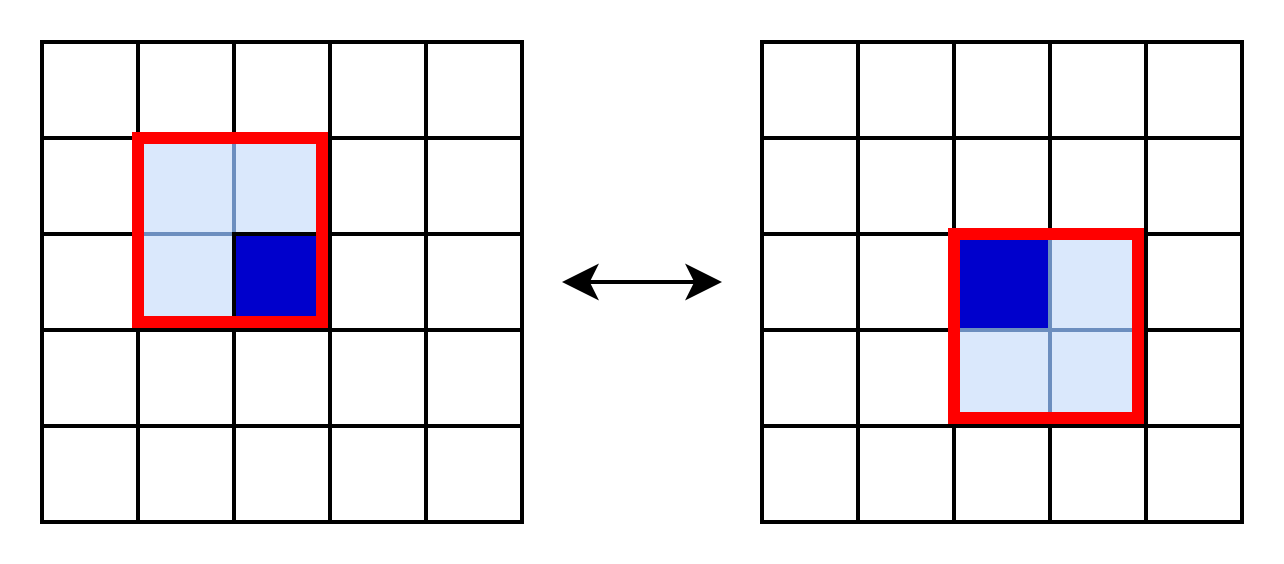
\includegraphics[width=0.6\textwidth]{obrazky-figures/ch2/Margolus.png}
    \caption{Margolusovo okolí (tmavě modrá = zkoumaná buňka, červená = 2x2 blok, světle modrá = okolí).}
    \label{fig:Margolus}
\end{figure}

Posledním, zde zmíněným, důležitým vědcem v historii CA byl Stephen Wolfram, který, jak již bylo zmíněno, ve své knize \textit{A New Kind of Science}~\cite{wolfram-NewKindOfScience} popsal 4 třídy pro klasifikování celulárních automatů a to podle jejich vztahům k druhému na základě fyzikálního zákonu zachování hmotnosti.

\subsection*{Využití celulárních automatů ve hrách}
Jedním z využití CA obsahují hry \uv{padajícího písku}, neboli \textit{Falling-sand games/simulators}. Tyto hry jsou nejčastěji 2D, sandboxové (= podporující kreativitu), jsou založeny například na blokovému/rozdělujícímu celulárnímu automatu, které mohou simulovat reálnou fyziku, jelikož jsou reverzibilní a dodržují fyzikální zákon zachování hmot~\cite{schiff2011cellular}. Nejjednodušší okolí využívané na vyhodnocení těchto CA je Margolusovo (viz obrázek~\ref{fig:Margolus})\,--\,2D mřížka je rozdělena na 2x2 čtverce, které se každou generaci posouvají diagonálně o jednu buňku~\cite{schiff2011cellular} (okolí v čase t se tedy skládá ze všech buněk, které se nacházejí v bloku v aktuálním čase).

\noindent Hráč má při hraní hry přístup k několika materiálům/elementům, které mají každý své vlastní vlastnosti (gravitace, reaktivnost s jinými materiály), se kterými může interagovat na dané ploše. Příkladem těchto her může být The Powder Toy~\footnote{https://powdertoy.co.uk}, The Sandbox (2012), Sandspiel (ukázka na obrázku~\ref{fig:Sandspiel}) či Noita (hra doplněná o roguelike aspekt).
\begin{figure}[H]
    \centering
    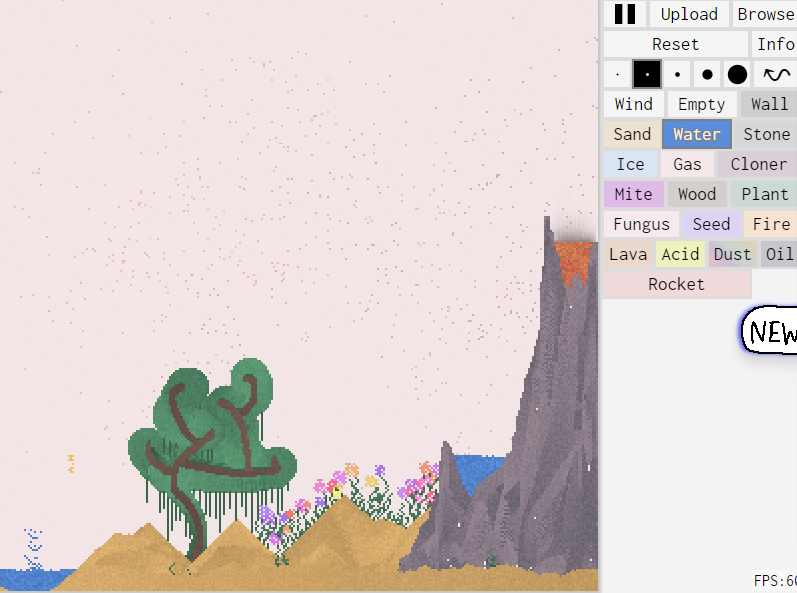
\includegraphics[width=0.5\textwidth]{obrazky-figures/ch2/SandSpiel.png}
    \caption{Ukázka ze hry Sandspiel.}
    \label{fig:Sandspiel}
\end{figure}

\begin{figure}[H]
    \centering
    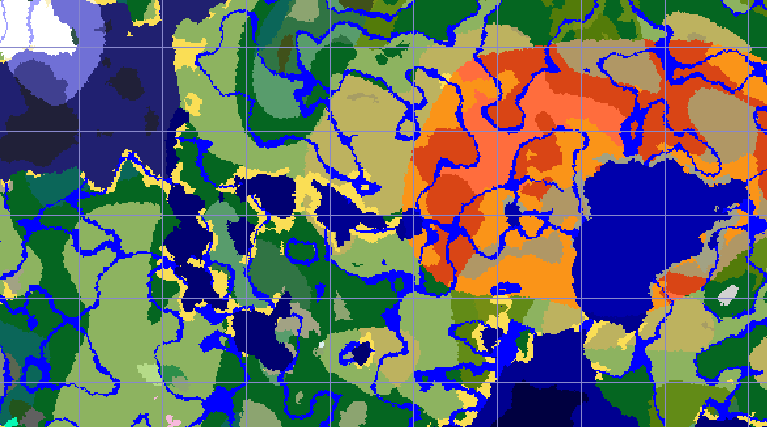
\includegraphics[width=0.7\textwidth]{obrazky-figures/ch2/minecraft_biom.png}
    \caption{Příklad vygenerovaného Minecaft světa s různými biomy}
    \label{fig:minecraft_biom}
\end{figure}

Rozšířenější, a v moderních hrách i častější, je využití CA na procedurální generování terénu\,--\,to je možné najít ve hrách jako je Tje využit u her vyžadujících větší a pestrý svět, či vysoký počet úrovní vyžadujících rozmanité překážky. Je to, jelikož klasické \uv{lidské} výtvory mohou být drahé 2 způsoby. Manuální navrhovaní obrovské mapy, či 100+ úrovní lidmi zabere mnoho času, energie a může naskytnout repetitivita, také tyto před-vytvořené mapy zabírají mnoho paměti a jejich načítaní může být obtížné na procesor\,--\,procedurální generace tedy vytváří mapy za chodu aplikace, takže vyřeší oba problémy~\cite{Procedural_Game_Map}.

Minecraft například generuje základ své mapy díky stochastickým celulárním automatům spuštěných nad zpracovanými (např. pomocí šumu) výsledky kongruentních generátorů~\cite{Minecraft}. Stochaistické/Náhodné celulární automaty, jsou CA u nichž nejsou pravidla deterministická (tj. nepředvídatelná), ale pravděpodobnostní\,--\,to znamená, že místo pevného pravidla určujícího následující stav buňky má zadané pravděpodobnosti možných nových stavů buňky~\cite{DBLP:journals/corr/abs-1304-7185}. Díky tomuto dochází k definování přechodů a prolínání mezi různými poddruhy biomů (příklad vygenerované mapy je vidět na obrázku~\ref{fig:minecraft_biom}). Například teplé oblasti mají 50\% šanci, že se promění v poušť, 33\% v savanu a 17\% v roviny, nebo oceány mající 50\% šanci, že se promění v zem~\cite{Minecraft}.

Některé z jednodušších možností generování prostředí s celulárními automaty je využití algoritmů na náhodné generování jeskyní. Příkladem může být například algoritmus (zapsán níže algoritmem \ref{algo:cave_gen}) z naučné stránky envatotuts+~\cite{CaveCA}, kde buňka CA může nabývat 2 stavů\,--\,živá, mrtvá, jehož výsledek je na obrázku~\ref{fig:cave}.
\begin{algorithm}
\caption{Generování jeskyní pomocí CA}\label{algo:cave_gen}
\begin{algorithmic}[1]
\State \textbf{Input:} $\text{matrix}, \text{row}, \text{col}, \text{deathLimit}, \text{birthLimit}$
\State \textbf{Output:} updated state of the cell
\State $\text{neighbors} \gets \text{countAliveNeighbours}(\text{matrix}, \text{row}, \text{col})$
\State $\text{cellValue} \gets \text{matrix[row][col]}$
\If{$\text{cellValue} = \text{alive}$}
    \If{$\text{neighbors} < \text{deathLimit}$} \Comment{Too many neighbours} 
        \State \textbf{return} $\text{dead}$
    \Else
        \State \textbf{return} $\text{alive}$
    \EndIf
\Else
    \If{$\text{neighbors} > \text{birthLimit}$} \Comment{Reborn} 
        \State \textbf{return} $\text{alive}$
    \Else
        \State \textbf{return} $\text{dead}$
    \EndIf
\EndIf
\end{algorithmic}
\end{algorithm}
\newline
Algoritmus funguje na několika jednoduchých principech, s nimiž je možné různě manipulovat, a to změnou hodnot \verb|deathLimit| a \verb|birthLimit|:
\begin{itemize}
    \item narození = pokud je buňka mrtvá a má určitý počet živých sousedů, v následující iteraci oživí (podpora růstu jeskynních chodeb),
    \item smrt = pokud je buňka živá a má příliš málo mrtvých sousedů, zemře v následující iteraci (vytváření otevřených prostorů v jeskyni),
    \item přežití = pokud je buňka živá a má dostatečný počet živých sousedů, přežívá do následující iterace (udržování existující struktury jeskyní).
\end{itemize}

\begin{figure}[H]
    \centering
    
\includegraphics[width=0.5\textwidth]{obrazky-figures/ch2/cave.png}
    \caption{Příklad algoritmu generování jeskyní s využitím Moorova okolí,	deathLimit = 3, birthLimit = 4.}
    \label{fig:cave}
\end{figure}

Také je možné využít algoritmy, generující strukturu podobnou bludišti. Celulárním automatem s touto vlastností je OCA:Maze~\cite{OCA:Maze}. Hlavním principem tohoto algoritmu s~Mooreovým okolím je, že pokud má buňka živých 1 až 5 sousedů tak přežije a ožívá pokud má přesně 3 sousedy\,--\,to znamená, že je pro buňky složitější zemřít a tím se vytváří vzory podobné bludišti, jak je vidět v levé částí obrázku~\ref{fig:OCA:Maze}. Při generování s náhodnou matici, ale nejsou cesty zcela propojené, získáváme jen mnoho nepropojených místností. Existuje i~jeho upravená verze (Mazectric), která ale omezuje počet sousedů potřebný přežití na 1~až~4, díky čemuž vznikají rovnější a delší \uv{cesty}~\cite{OCA:Maze}, což je možné vidět na pravé částí obrázku~\ref{fig:OCA:Maze}.
\begin{figure}[H]
    \centering
    
\includegraphics[width=0.47\textwidth]{obrazky-figures/ch2/OCA:Maze.png}\hspace{0.5cm}
    
\includegraphics[width=0.47\textwidth]{obrazky-figures/ch2/Mazectric.png}
    \caption{Porovnání výsledků CA OCA:Maze (vlevo) a Mazectric (vpravo).}
    \label{fig:OCA:Maze}
\end{figure}
    
%--------------------------
% Prohledávání stavového prostoru
\section{Prohledávání stavového prostoru}
Stavový prostor (anglicky \textit{State space}), využívaný na řešení úloh, lze v informatice popsat jako orientovaný graf, v němž jeho uzly reprezentují stavy, a hrany reprezentují operátory, či stavové přechody~\cite{State-Space_Search}. Formálně je možné stavový prostor a jeho aktuální řešenou úlohu zapsat jakožto čtveřici (S, O, $s_0$, G), jejíž prvky zde definovat jako~\cite{izu}:
\begin{itemize}
    \item S je množina všech možných stavů,
    \item O je množina všech přechodů mezi stavy/operátorů, kterými lze měnit stavy,
    \item $s_0$ je počáteční stav řešené úlohy, $s_0 \in S$,
    \item G je neprázdná podmnožina S cílových stavů úlohy.
\end{itemize}
Úlohy lze řešit díky neinformovaným/slepým metodám, nebo informovaným metodám, které jsou popsány níže. 

\subsection*{Neinformované metody}
Nazývají se neinformovanými neboli slepými, jelikož nemají žádné začáteční informace o~prostoru a umístění cíle. Což znamená, že tyto vyhledávající metody systematicky prohledávají stavový prostor, dokud nenajdou zadaný hledaný výsledek, který do té doby ani neberou v úvahu, pouze pokračují v \uv{prolézání} prostorem~\cite{poole2023artificial} (či neúspěšně prohledají všechny části stavového prostoru). Dále v kapitole jsou popsány některé příklady metod tohoto typu.

\subsubsection*{\textbullet Metoda slepého prohledávání do šířky (BFS)}
Metoda funguje na principu fronty FIFO (\textit{= first-in, first-out}) do které postupně zapisuje uzly, které jsou objeveny, ale neprohledány~\cite{poole2023artificial}. 

\begin{figure}[H]
    \centering
    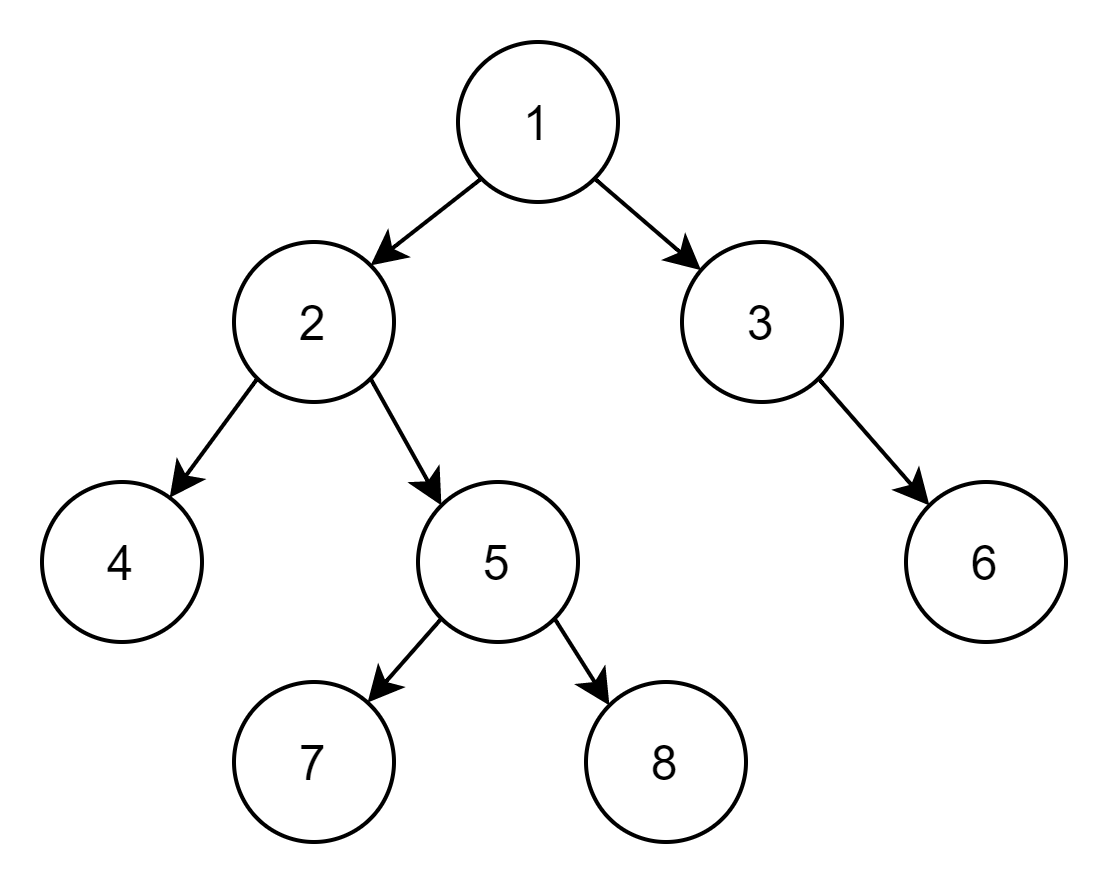
\includegraphics[width=0.48\textwidth]{obrazky-figures/ch2/BFS.png}\hspace{0.25cm}
    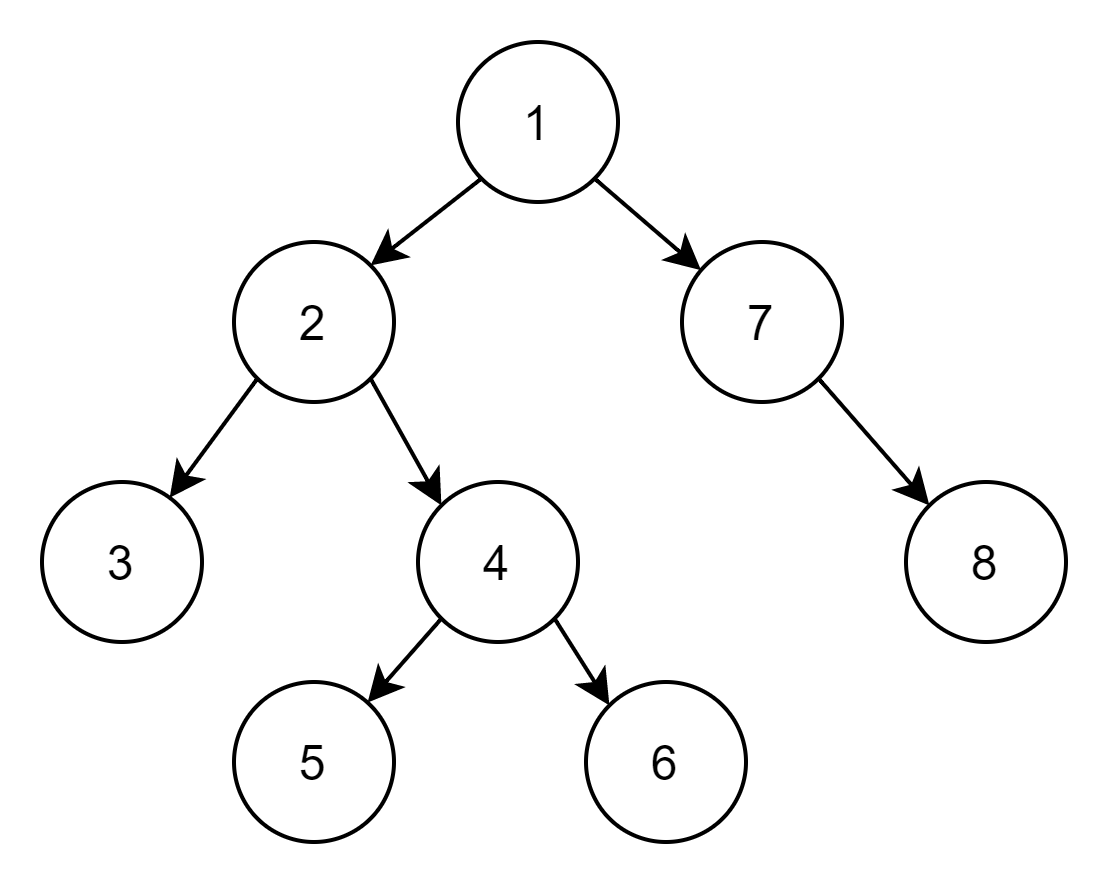
\includegraphics[width=0.48\textwidth]{obrazky-figures/ch2/DFS.png}
    \caption{Porovnání metod prohledávání stavového prostoru BFS (vlevo) a DFS (vpravo).}
    \label{fig:BFS_DFS}
\end{figure}

Prohledávání začíná v kořeni, neboli startovním uzlu, a postupně po úrovních, prochází prvně sousedy kořene, následně sousedy jeho sousedů, atd. dokud nedojde k cíli (zadaný hledaný uzel), od kterého navrátí nejkratší cestu až ke kořeni~\cite{Introduction_to_Algorithms}, či dokud neprohledá neúspěšně celý prostor. Výsledek prohledávání je možné vidět vlevo na obrázku~\ref{fig:BFS_DFS}

Časová složitost je \(\mathcal{O}_{BFS} = |V| + |E|\), kde \(|V|\) je součet počtu uzlů a \(|E|\) je počet hran~\cite{CS225BFSDFS}.

\subsubsection*{\textbullet Metoda slepého prohledávání do hloubky (DFS)}
Metoda pracující se zásobníkem LIFO (\textit{= last-in, first-out}), který využívá k \textit{backtrackingu}, neboli navrácení~\cite{poole2023artificial}. Stejně jako BFS začíná v kořeni, od kterého ale jde do hloubky. To znamená, že vybere jeden neprozkoumaný synovský sousední uzel, u kterého vybere jeho neprozkoumaný synovský sousední uzel a takto pokračuje, dokud nedorazí na \uv{dno}, tedy do místa, kde už nemůže pokračovat hlouběji do dalších sousedů\,--\,v tomto případě se pomoci, již zmíněného, \textit{backtrackingu} navrátí k nejbližšímu otcovskému sousedovi, u kterého ještě nebyly prozkoumány všechny sousedské uzly a prohledává dál~\cite{Introduction_to_Algorithms}. Toto pokračuje, dokud nenajde hledaný cílový uzel, nebo dokud neprojde celý prostor bez nalezení cíle. Ukázka průchodu stromem je v pravé části obrázku~\ref{fig:BFS_DFS}.

Stejně jako u BFS, časová složitost je \(\mathcal{O}_{DFS} = |V| + |E|\), kde \(|V|\) je součet počtu uzlů a \(|E|\) je počet hran~\cite{CS225BFSDFS}.

\subsubsection*{\textbullet Metoda postupného zanořování do hloubky (IDS)}
Tato metoda je kombinací BFS a DFS, což znamená, že prohledávání funguje stejně jako u~DFS s výjimkou, že algoritmus postupuje po úrovních a postupně zvyšuje limit hloubky~\cite{poole2023artificial}. Tedy při první iteraci prohledává hloubkově pouze první úroveň, poté co je celá prohledaná postupuje na druhou iteraci, při které už vstupuje i do druhé atd. dokud nenajde cíl, či nevyčerpá celý stavový prostor. 

IDS se využívá pokud nemůžeme stanovit hloubku řešení a jeho časová složitost je \(\mathcal{O}_{IDS}(b^{d})\), kde \(b\) je faktor větvení (průměrný počet následovníků uzlu) a \(d\) hloubku optimálního řešení~\cite{izu}.

\begin{figure}[H]
    \centering
    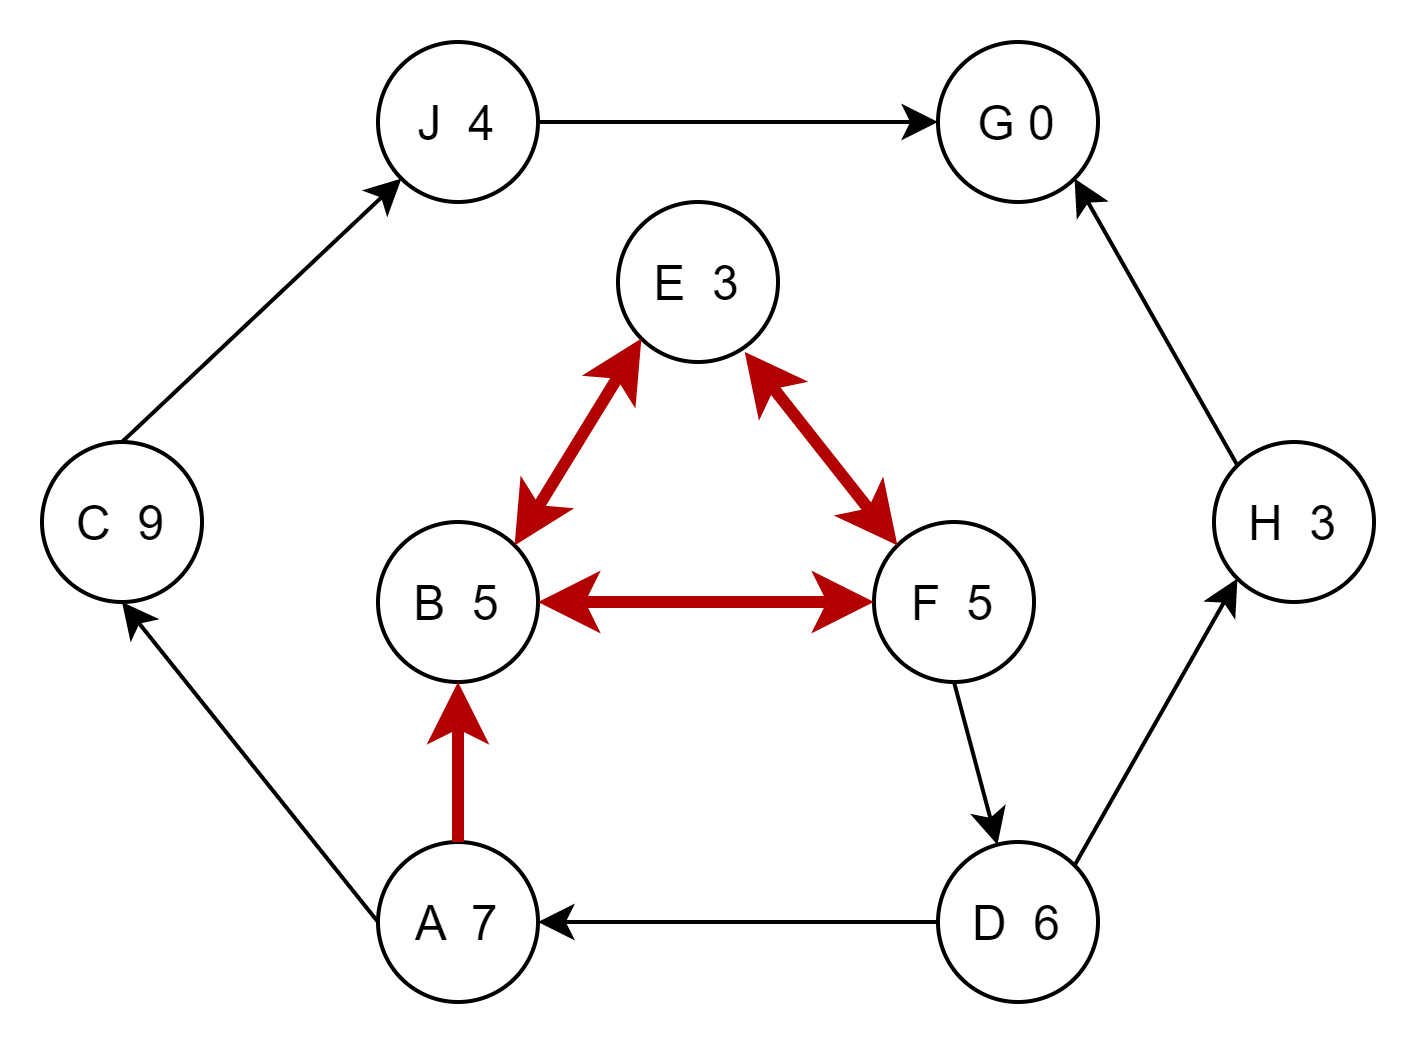
\includegraphics[width=0.7\textwidth]{obrazky-figures/ch2/GreedySearch.png}
    \caption{Nespolehlivost metody hladového prohledávání při hledání cesty z A do G, červeně zvýrazněno cyklení (uzly ve formátu [název uzlu, heuristika]).~\cite{poole2023artificial}}
    \label{fig:GreedySearch}
\end{figure}

\subsection*{Informované metody}
Informované metody na rozdíl od neinformovaných znají polohu cíle~\cite{izu}, kterou využívají na zhodnocení cesty pomocí funkce  ${f(n)}$, kde ${n}$ je stav/uzel. Tyto metody jsou také nazývány heuristickými, jelikož využívají k dosáhnutí cíle heuristickou funkci\,--\,díky této funkci ${h(n)}$ lze vypočítat pomocí uzlu ${n}$ nezáporné reálné číslo značící odhad nákladů na cestu z uzlu ${n}$~do uzlu cílového~\cite{poole2023artificial}. Čím menší je výsledné číslo, tím pravděpodobněji povede k cílovému uzlu a tedy ${h(n) = 0}$, ${n}$ je cílovým uzlem~\cite{AI-Modern_approach}.

\subsubsection*{\textbullet Metoda hladového prohledávání}
Anglicky nazývaný \textit{Greedy search}, je jeden z nejlehčích přístupů, jelikož využívá na zhodnocení uzlu pouze heuristickou funkci, tedy ${f(n) = h(n)}$~\cite{AI-Modern_approach}. Další krok od aktuálního uzlu se rozhoduje pouze v závislosti na této funkci, tedy hrana s nejmenší heuristikou, čímž může dojít k chybnému výsledku\,--\,metoda hladového prohledávání negarantuje nalezení výsledku~\cite{poole2023artificial}. 

Chybný postup k výsledku můžeme vidět v obrázku~\ref{fig:GreedySearch}, na kterém se nachází příklad z knihy \uv{Artificial Intelligence: Foundations of Computational Agents}~\cite{poole2023artificial}, kde při snaze nalezení cesty z uzlu A do uzlu G zůstane algoritmus zacyklen v uzlech B, E, F.

\subsubsection*{\textbullet Metoda A*}
Metoda A* vyhodnocuje další krok na základě hodnotící funkce ${f(n) = g(n) + h(n)}$, kde ${g(n)}$ udává cenu cesty z předešlého do uzlu ${n}$ a ${h(n)}$ je heuristická funkce~\cite{AI-Modern_approach}. 

Pro správnou funkci A* algoritmu je důležité zvolit přípustnou (anglicky \textit{admissible}) heuristiku, což je heuristika, u které cena cesty z uzlu ${n}$ do cílového uzlu nikdy nepřeceňuje cenu ze startovního uzlu k cílovému~\cite{AI-Modern_approach, izu}. Jednou z přípustných heuristik, je přímá euklidovská vzdálenost mezi 2 uzly~\cite{poole2023artificial}, která vhodná na využití u prostorových problémů s přesnými rozměry (např. 2D mřížkový prostor, bez překážek, se 4 povolenými směry - nahoru, dolu, doleva, doprava). Pokud algoritmus při jeho výpočtu dorazí k výsledku heuristické, který by toto nesplňoval, využívá \textit{backtracking} a pokračuje cestu k dalšímu nejlepšímu uzlu.

Podobně jako u metody hladového prohledávání hledá algoritmus cestu po nejmenších hodnotách, ale díky využití kombinace ${g(n)}$ a ${h(n)}$ je algoritmus řazen jako přípustný (vždy, když existuje, vrací optimální řešení)~\cite{poole2023artificial}.
    
%--------------------------
% Rejection sampling
\section{Rejection sampling}
Rejection sampling, či metoda accept-reject (česky přijetí-odmítnutí), je metoda vzorkování využívaná ke generování náhodných proměnných~\cite{thomopoulos2012essentials} a na vzorkování dat ze sofistikované, neboli obtížně vzorkovatelné, distribuce~\cite{Sachdeva_2021}.

Základní myšlenkou rejection samplingu je, že místo přímého vzorkování komplikované funkce f(X) můžeme generovat vzorky pomocí jednodušší distribuce Q(X), ty následně překontrolovat, zda patří do funkce komplikovanější~\cite{ghojogh2020sampling} a na základě toho je přijmout, či pokud do ní nepatří, odmítnout. Vizuální příklad je možné vidět na obrázku~\ref{fig:RA_graph}, který vyobrazuje vzorky vygenerované na základě funkce Q(X). Vzorky nacházející se v území patřící pod funkci f(X) a označené zelenou barvou, budou akceptovány a body mimo (označené žlutě) jsou odmítnuty.

\begin{figure}[H]
    \centering
    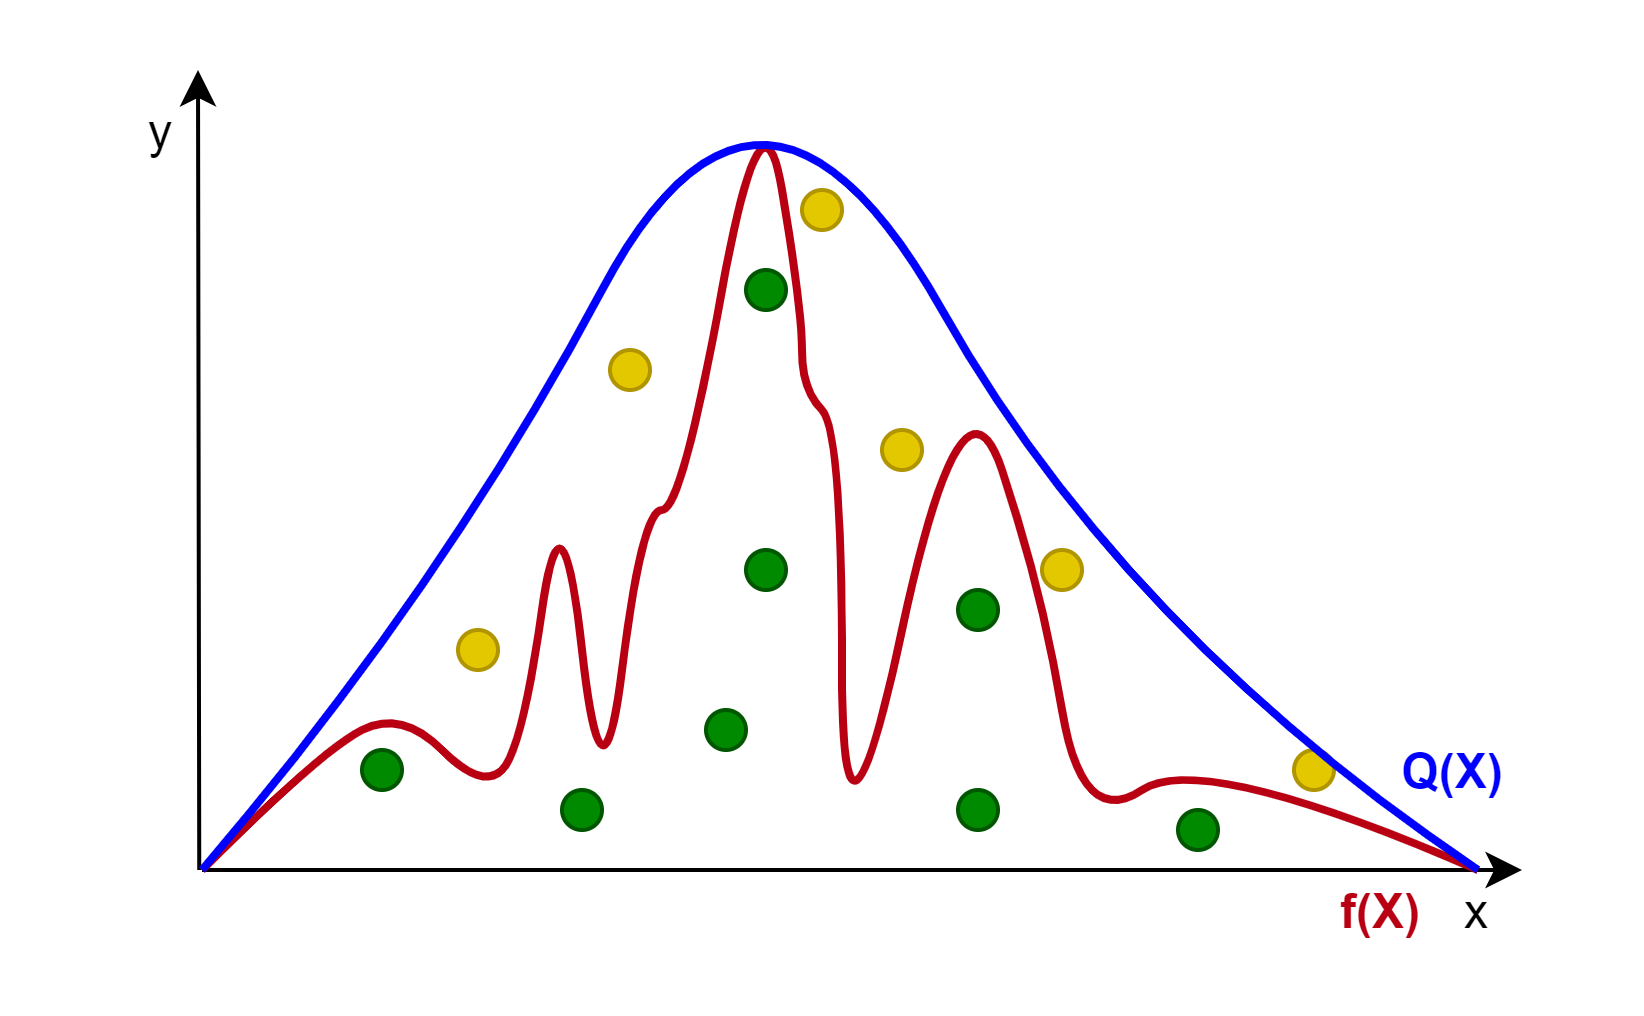
\includegraphics[width=\textwidth]{obrazky-figures/ch2/RA_graph.png}
    \caption{Příklad Rejection samplingu, kde jsou díky využití jednodušší distribuce Q(X) (modrá) získány vzorky ze složitější funkce f(X) (červená)}
    \label{fig:RA_graph}
\end{figure}

Pro detailnější vysvětlení je využit algoritmus~\ref{algo:rejection_sampling} sepsaný podle výukového a literárního přehledu z Univerzity Waterloo~\cite{ghojogh2020sampling} a edukační stránky~\cite{Sachdeva_2021}. V tomto algoritmu je $\mathcal{S}$ sada vzorkovacích dat o velikosti $n$, která se postupně naplňuje generovanými daty, které jsou vzorky složitější funkce f(X). V cyklu generujícím a potvrzujícím vzorky je prvně vytvořen vzorek $x$ z funkce Q(X) a následně vzorek $u$ z rovnoměrného rozložení $U(0, c\, Q(x_i))$. Škálovací konstanta $c$ je využívána k určení horních mezí pro přijetí nebo odmítnutí vzorku a platí, že $c \cdot Q(X) \geq f(x) \ \text{pro všechny } x$.
\label{eq:RA_c}
\begin{algorithm}[h]
\caption{Rejection sampling/Accept-reject}\label{algo:rejection_sampling}
\begin{algorithmic}[1]
    \State \textbf{Input:} $f(x), Q(X), c$\;
    \State \textbf{Output:} $\mathcal{S}$
    \State $\mathcal{S} \gets \varnothing$
    \For{$i = 1$ to $n$}
        \State $x_i \sim Q(X)$
        \State $u_i \sim U(0, c\, Q(x_i))$
        \If{$u_i < f(x_i)$}
            \State Accept $x_i$: $\mathcal{S} \gets \mathcal{S} \cup \{x_i\}$
        \Else
            \State Reject $x_i$: $i \gets i - 1$
        \EndIf
    \EndFor
\end{algorithmic}
\end{algorithm}
\todo{malé/velé x?}
%===---------------====
% KONCEPT
%===---------------====
\chapter{Koncept 2D labyrintové hry}
\todo{Dopsat - popsat koncept typu her obecně (pravidla labyrintových her,..)}
    
%--------------------------
% Úvod
\section{Úvod do hry/cíle/myšlenka}
\todo{popsat návrh přístupu k problému (zadání), asi taky grafík -> jak jsem postupovala}
%--------------------------
% Mechaniky hry
\section{Mechaniky hry}
\todo{mapa, obecne o hre- princip hry (nekonecna, zvysujici se narocnost)}
\subsection*{Úrovně}
\todo{zvysovani urovni (zde nejaky graf)}
\subsection*{Hráč}
\todo{kamera -> proc jsem vybrala jen cast, ovladani, grafika}
\subsection*{Nepřátelé}
\subsection*{Další objekty}
 
%--------------------------
% Uživatelské rozhraní
\section{Uživatelské rozhraní}
\todo{FIGMA (asi strana plná obrázků + popis proc}

%===---------------====
% IMPLEMENTACE
%===---------------====
\chapter{Implementace 2D labyrintové hry} % TODO NECO KONKRETNEJSIHO
Pro implementaci hry bylo otestováno několik game enginů a zváženy jejich výhody a nevýhody. Jelikož cílem bylo vytvořit jednoduchou 2D hru jejíž hlavním a nejsložitějším bodem je mapa nyl vybrán Godot verze 4. 

Tato platforma byla zvolena oproti jiným možnostem díky její široké a jednoduché podpoře vytváření 2D her. Například Unreal Engine, která je zaměřená spíše na realistické 3D světy. Jak je již zmíněno v kapitole o Godotu, tento herní engine na rozdíl od Unity či Unreal Engine využívá vlastní skriptovací jazyk GDScript, podobný syntaxí pythonu, který díky svým knihovnám ulehčuje manipulaci s herními prvky (nodes) a urychluje tak vývoj.

Nejdůležitější vlastností Godotu pro vyváření této hry a její základní mapy byla node \uv{TileMap}, která slouží pro vytváření 2D dlaždicových map. Její využití je popsáno v následujících podkapitolách.
    
%--------------------------
% Generování mapy
\section{Generování mapy}
\todo{mock up grafík}
\subsection*{Kostra bludiště}
CA
\subsection*{Propojení bludiště}
GRAFOVÉ ALGORITMY

%--------------------------
% Hráčská postava a její umístění
\section{Cesta bludištěm} % start + cil

%--------------------------
% Experimenty s generováním map pomocí CA
\newpage
\section{Experimenty s generováním map} % statistiky, proc jsem vybrala dany postup
\todo{statistiky v generovani mistnosti, po propojeni obsah zdi vs cest + kolik CA generaci na plno - jak na kolika, proc, rovnice}

\begin{table}[htbp]
    \centering
    \caption{Výsledky experimentu s mapou}
    \label{tab:map_experiment}
    \begin{tabular}{|c|c|c|c|c|}
    \hline
    a & Mazetric\_1\_1 & Mazetric\_3\_2 & Cave\_Mazetric\_1\_1 & Cave\_Mazetric\_3\_2 \\ \hline
    5  & \textbf{0,858}         & 0,860          & 0,890                 & 0,886                \\ \hline
    10 & \textbf{0,859}          & 0,861          & 0,862                 & 0,860                \\ \hline
    15 & 0,856          & \textbf{0,852}          & 0,855                 & 0,856                \\ \hline
    20 & \textbf{0,847}          & 0,851          & 0,854                 & 0,851                \\ \hline
    25 & 0,845          & 0,847          & \textbf{0,849}                 & 0,847                \\ \hline
    30 & 0,845          & 0,843          & \textbf{0,847}                 & 0,846                \\ \hline
    35 & 0,841          & 0,841          & \textbf{0,845}                 & 0,843                \\ \hline
    40 & 0,840          & 0,839          & \textbf{0,844}                 & 0,842                \\ \hline
    45 & 0,838          & 0,838          & 0,841                 & \textbf{0,842}                \\ \hline
    50 & 0,838          & 0,838          & 0,839                 & \textbf{0,840}                \\ \hline
    \end{tabular}
\end{table}

\begin{equation}
    \text{Efektivita} = \left(1 - \frac{g}{\text{a}^2}\right) \cdot \alpha + \left(\text{p} \cdot \beta \right)
\end{equation}

kde: 
\begin{itemize}
    \item $g$ je průměrný počet skupin ve 100 instancích bludiště
    \item $a$ je velikost 1 strany zkoumaného bludiště ($a^2$ je obsah čtvercového bludiště)
    \item $\alpha$ je konstanta\,--\,váha důležitosti přidělena počtu skupin = $0,85$
    \item $\frac{g}{\text{a}^2}$ označuje složitost vytvořeného bludiště
    \item $p$ označuje poměr mezi nejkratší cestou od začátku ke konci a zbytkem cest (políček na které jde vstoupit)
    \item $\beta$ je konstanta\,--\,váha důležitosti poměru cest = $0,15$
\end{itemize}
do 20 beru nejnižší hodnotu, od 20+ beru nejnižší hodnotu -> vizuální odhad, menší bludiště potřebují víc cest, větší už jsou chaotické dost, ulehčujeme to
 méně skupin vede k většímu výsledku
  hustší cesty vedou k většímu výsledku
\newpage
%--------------------------
% Nepřátelé, objekty a jejich rozmístění
\section{Nepřátelé, objekty a jejich rozmístění}

%--------------------------
% Úrovňový systém
\section{Úrovňový systém}

\subsection*{Skóre}

%===---------------====
% TESTOVANI
%===---------------====
\chapter{Uživatelské testování}
Uživatelské testování bylo prováděno formou online anonymního dotazníku (Google Forms), který testované subjekty vyplnily po otestování alfa verze hry. Hra byla testována na počítačích s Windows a Linux operačními systémy. Testery byli aktivní i nezkušení hráči her, naverbováni primárně díky sdílení testovacích prostředků na sociálních sítích.
%--------------------------
% Dotazník
\section{Dotazník}
Otázky byly vytvořeny k testování hlavních aspektů hry, jako je hratelnost, uživatelské rozhraní, stabilita programu a celková náročnost. Dotazník je navržen tak, aby umožňoval rychlé vyhodnocení prostřednictvím výběru z několika otázek s předdefinovanými možnostmi/škálami a pár otevřených otázek, a to kvůli využití hromadného testování. Otázky a~jejich typ je vypsán v tabulce~\ref{tab:questions}.

\begin{table}[h]
    \centering
    \begin{tabularx}{\textwidth}{X | X}
    \hline
    \textbf{Otázka} & \textbf{Typ otázky} \\ \hline
    1. Kolik času jste strávili u hraní? & Otevřená otázka \\ 
    2. Jaká byla vaše nejvyšší dosažená úroveň (level)? & Otevřená otázka \\ 
    3. Jaký je váš celkový dojem ze hry? & Uzavřená otázka (velmi negativní--velmi pozitivní) \\ 
    4. Jak byste ohodnotili uživatelské rozhraní a celkovou přehlednost hry? & Uzavřená otázka (velmi nepřehledné--velmi přehledné) \\ 
    5. Jak byste ohodnotili stabilitu a výkon hry (záseky/pády, \ldots)? & Uzavřená otázka (velmi stabilní--nestabilní) \\ 
    6. Co pro vás bylo nejtěžší? & Polo-uzavřená otázka (orientace v bludišti, boj/vyhýbání se nepřátelům, technické chyby, ovládání, jiné:\ldots) \\ 
    7. Jak byste ohodnotili vyváženost zvyšující se obtížnosti? & Uzavřená otázka (velmi nevyvážená--velmi vyvážená) \\ 
    8. Pokud jste hodnotili hru jako spíše nevyváženou, jaký k tomu byl důvod? & Polo-uzavřená otázka (obtížnost se zvyšuje moc pomalu/rychle, na začátku moc jednoduchá a na konci moc složitá, jiné:\ldots) \\ 
    9. Jaké další funkce/vlastnosti/prvky byste ve hře ocenili/změnili? & Otevřená otázka\\
    \hline
    \end{tabularx}
    \caption{Seznam otázek}
    \label{tab:questions}
\end{table}

%--------------------------
\begin{figure}[H]
    \centering
    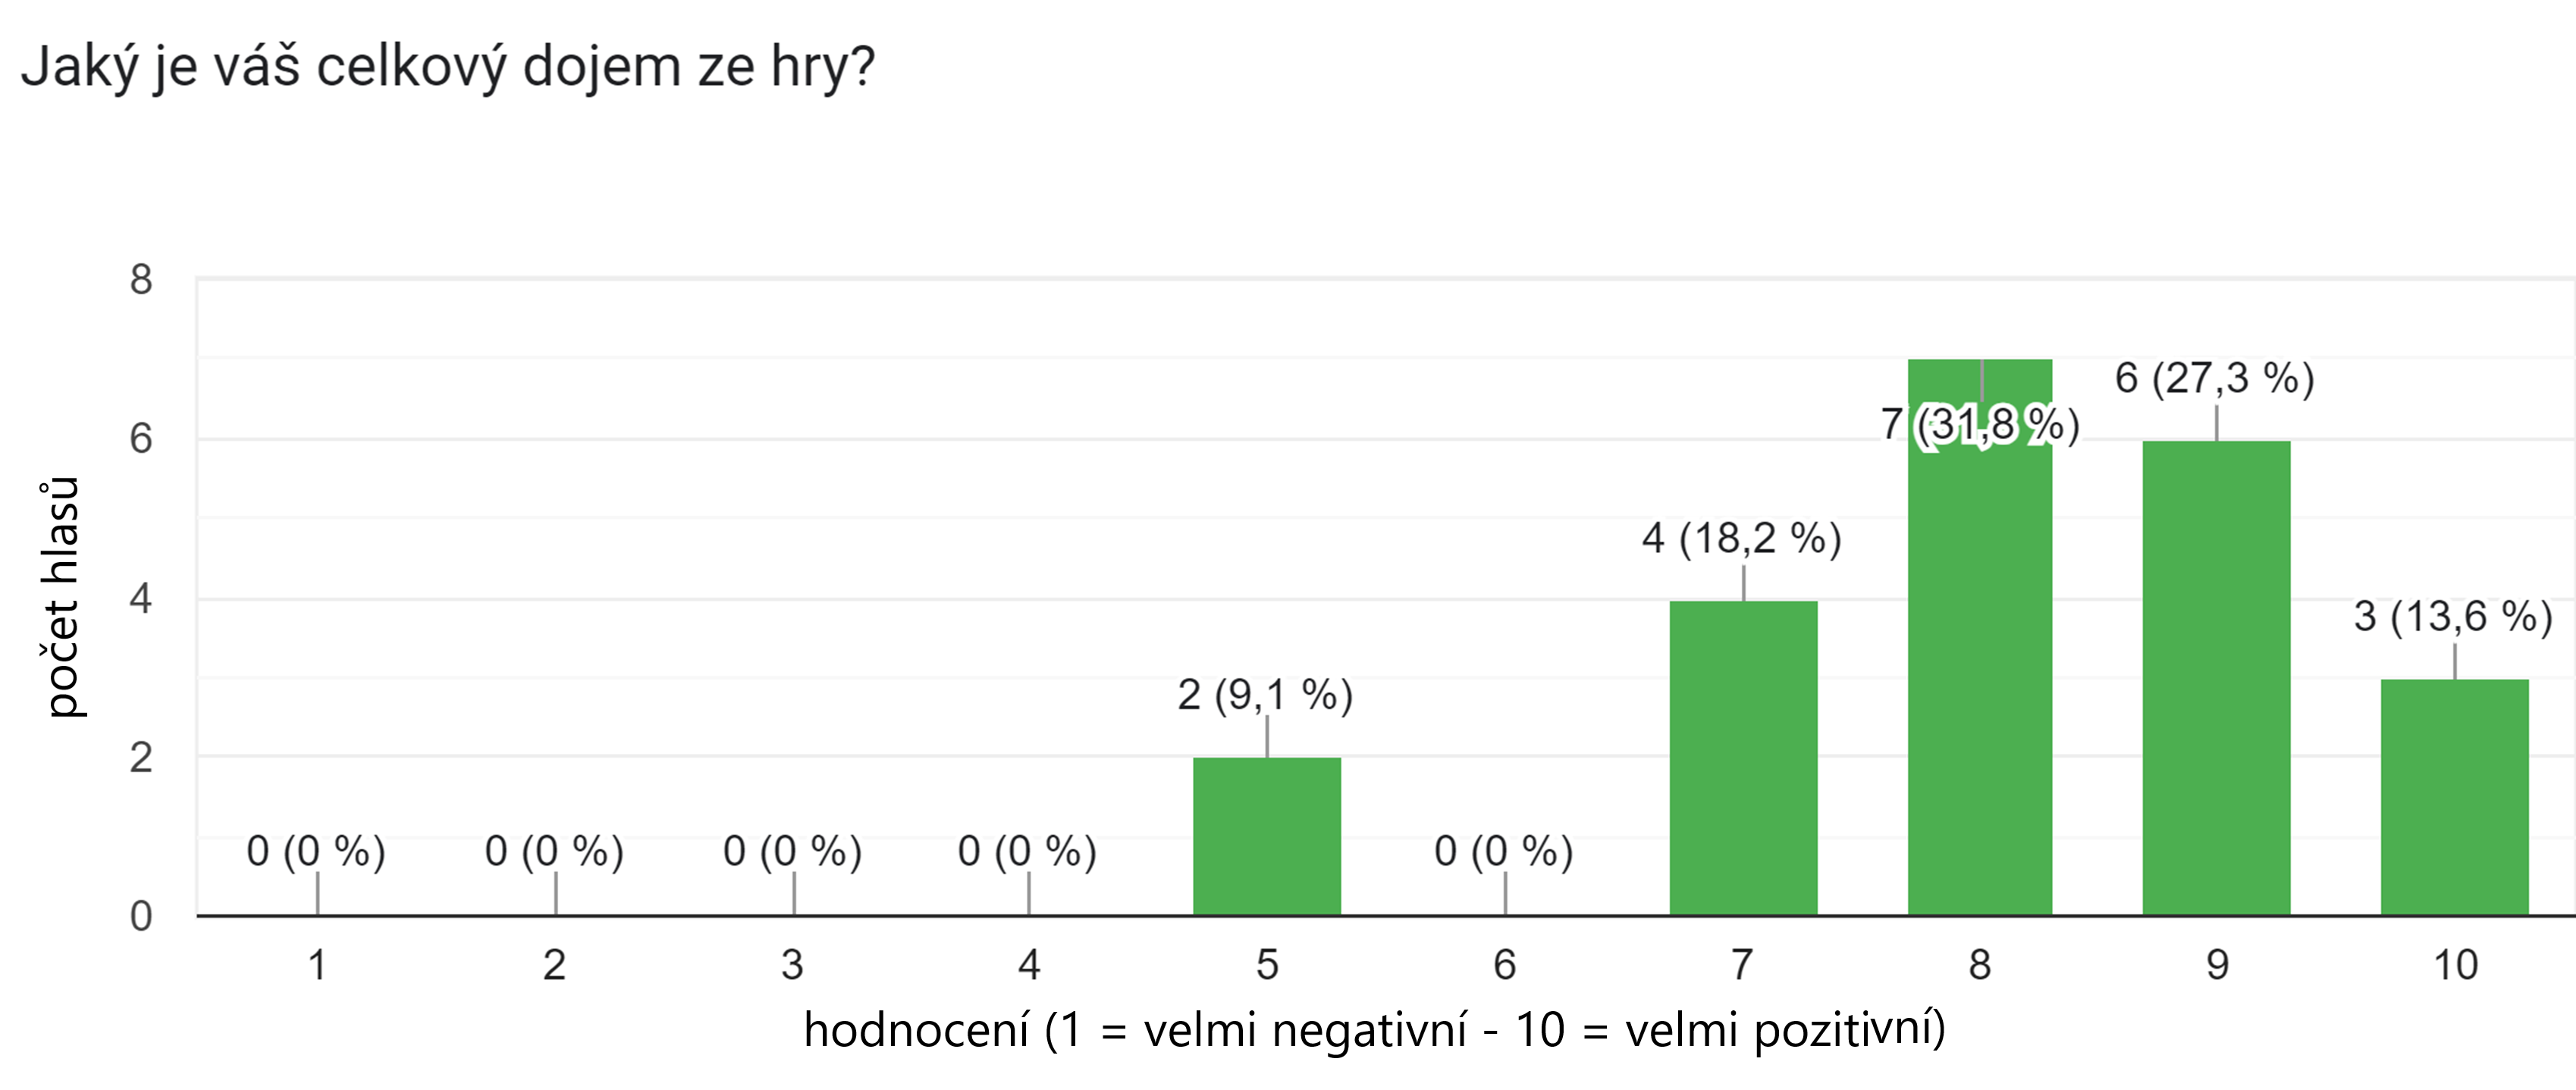
\includegraphics[width=\textwidth, height=0.25\textheight]{obrazky-figures/ch5/hodnoceni_celkovy_dojem.png}
    \caption{Graf odpovědí na otázku \uv{Jaký je váš celkový dojem ze hry?}.}
    \label{fig:hodnoceni_celkovy_dojem}
\end{figure}

% Analýza výsledků
\section{Analýza výsledků} \label{chap:Analýza výsledků}
Byly získány odpovědi od 22 subjektů, kompletní výpis všech odpovědí je dostupný v příloze~\ref{chap:user_testing}. Hráči strávili hraním hry průměrně půl hodiny s mediánem 20 minut. Průměrná úroveň, které dosáhli byla úroveň 14 a nejvyšší dosažený level byl 28.

\subsection*{Hratelnost}
Celkový dojem hráčů ze hry byl spíše kladný, jak je vidět na obrázku s grafem~\ref{fig:hodnoceni_celkovy_dojem}. Největší problém byl se způsobem počítání skóre, u kterého připouštím, že první verze nebyla dokonalá. Hlavním problémem bylo, že skóre bylo rozděleno dle stupňů, které nebyly rozděleny adekvátně, tak aby odpovídaly jejich společné časové náročnosti. To následně vytvořilo problém, že někteří hráči získávali za vyšší úrovně skóre záporné. Skóre se také občas špatně řadilo v tabulce výsledků. K tomuto jevy podle testerů docházelo, pokud bylo v tabulce více příspěvků se stejným jménem. Také se objevila stížnost na chybějící návod na ovládání.

Dalším problémem, na který několik testerů upozornilo byla absence legendy, či vysvětlení významu a vlastností objektů ve hře (předmětů a nepřátel). To také vyvolávalo zmatení u některých předmětů, jelikož hráči očekávali jinou funkci\,--\,například předmět truhly původně po sebrání jen zmizel bez dodatečných efektů, což u hráče vyvolalo zmatení, jelikož očekával, že dostane nějaký bonusový předmět, i přestože truhla dodává pouze bonusové skóre.

Objevilo se také několik drobných technických problémů, a to u kamery s pohledem na hráče, jenž dle recenzí testerů nebyla vhodně vycentrovaná a optimalizovaná pro rychlost hratelné postavy, kvůli čemuž se hráči setkávali s problémem že kamera \uv{nestíhala} zabírat postavičku při vertikálním pohybu a nastávaly neočekávané kolize se zdmi, pastmi nebo nepřáteli. To mohlo vést i k pocitu, že kamera zabírá moc malé území. Také si jeden tester povšiml, že hráčská postava se pohybuje diagonálně rychleji, než vertikálně a horizontálně, a že vyslání signálu útoku hráče není správně synchronizované s animací útoku, jelikož postava prvně zaútočí a odebere životy nepřátelům a následně se provede animace seknutí.

Hráči také vyjádřili své přání k budoucím implementacím pro zvýšení zábavnosti hry, těmito návrhy bylo například přidání hudby, či možnost úpravy hratelné postavy za získané skóre (jako měna).

\begin{figure}[H]
    \centering
    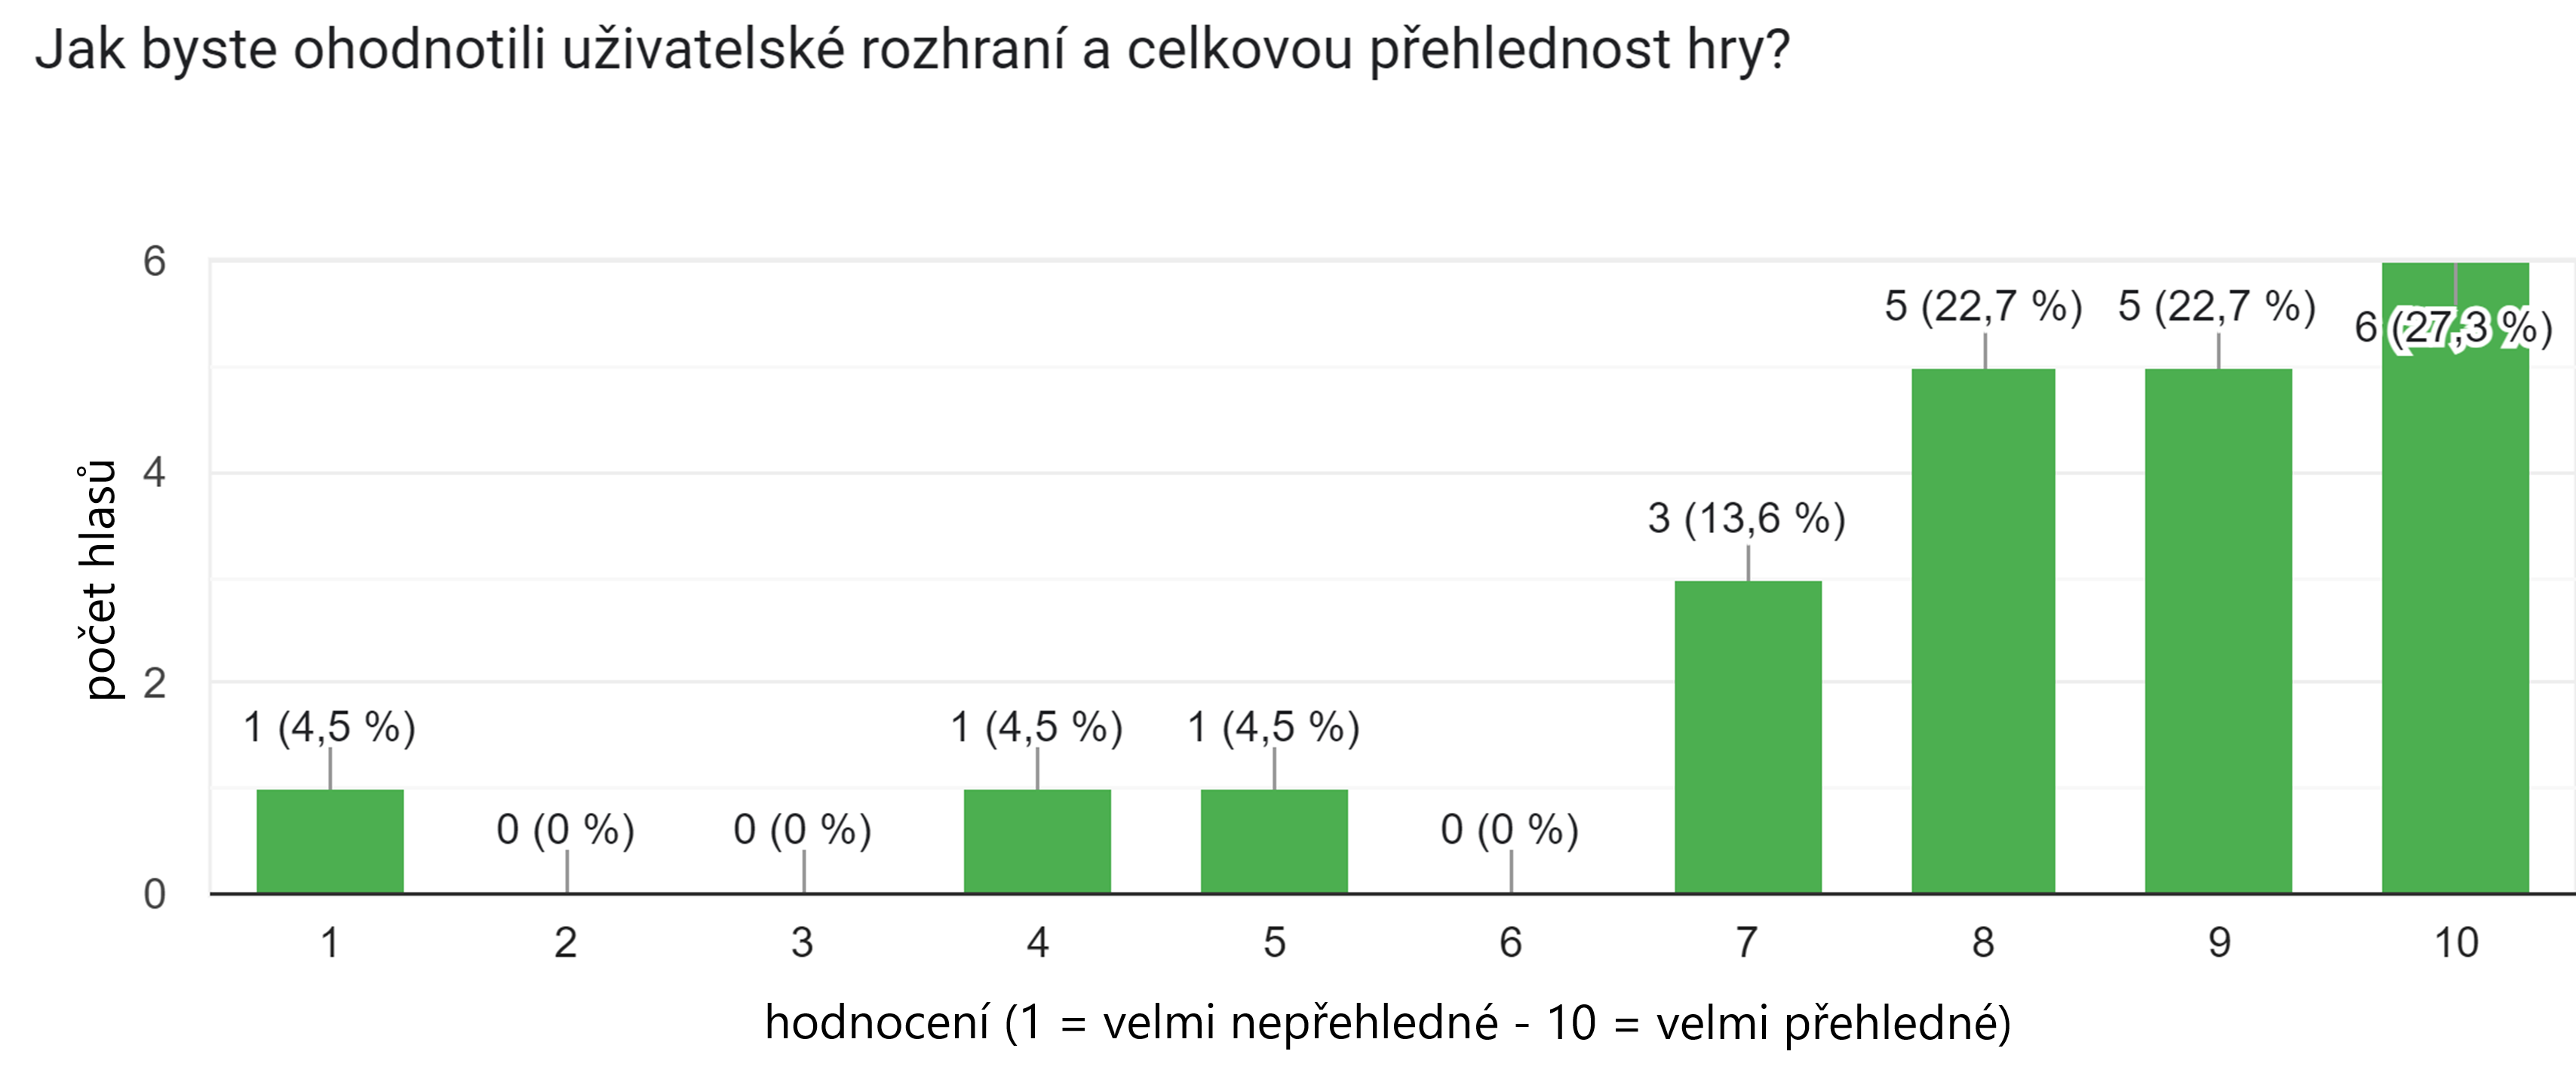
\includegraphics[width=\textwidth, height=0.25\textheight]{obrazky-figures/ch5/hodnoceni_ui.png}
    \caption{Graf odpovědí na otázku \uv{Jak byste ohodnotili uživatelské rozhraní a celkovou přehlednost hry?}.}
    \label{fig:hodnoceni_ui}
\end{figure}

\subsection*{Uživatelské rozhraní a grafická stránka hry}
Uživatelské rozhraní hodnotili testeři kladně, pouze s drobnými chybičkami\,--\,průměrný výsledek hodnocení je 8, tedy blíže k velmi přehledné s mediánem 8,5, jak je vidět na obrázku~\ref{fig:hodnoceni_ui}. Hráči oceňovali nápaditost a jednoduchost grafické a pixelové stránky hry. 

Nejčastěji opakovanou potřebou byla žádost na zobrazování skóre, či uběhlého času v úrovni, a ne pouze na konci u vyhodnocení, jelikož hráči byli zmatení nad způsobem počítání skóre. Na rozložení se objevila se pouze jedna stížnost testera, který byl zmatený umístěním srdíček, označující životy a jejich významem. Jiné stížnosti na rozložení nebyly, pouze jeden tester vyjádřil přání lepší viditelnosti zvoleného tlačítka, jelikož dle něj nebyl původní způsob dostatečně viditelný (byla pouze měněna barva textu tlačítka).

K ovládání se objevili stížnosti u hráčů hrajících pomocí šipek, jelikož ty jsou propojené i s ovládáním tlačítek v různých menu. Podle hráčů při vertikálnímu vstupu do portálu mohlo dojít k neočekávanému vypnutí hry, jelikož šipky ihned začali reagovat v ovládání menu. V otázce o dalších funkcích byla odpověď s návrhem na odchod z pauzy pomocí \textit{Esc} tlačítka. Jeden tester také vyjádřil žádost, aby se hra ihned po spuštění nedostávala do módu celé obrazovky, ale například jen do maximalizace, a to kvůli lepšímu manipulování při využití více obrazovek.

Pár drobných grafických úprav si dle testerů vyžádali i některé předměty, jako například meč (předmět zvyšující poškození) u kterého nebylo nijak jasné, že se násobní, nebo předmět truhly, který po jejím sebrání nedával nijak najevo jaký byl jeho význam. U pasti byl objeven problém s chybně vloženou texturou, takže se při hraní zobrazovala část textury jiné.

\subsection*{Stabilita programu}
Většina testerů (90\%, viz obrázek~\ref{fig:hodnoceni_stabilita}) označila hru jako stabilní a plynulou, nesetkali se tedy s žádným zbytečně dlouhým čekáním na generování nové úrovně, či pády hry.

Pouze 10\% (2 testeři) mělo drobné problémy, z nichž jeden se týkal pádu hry po zadaní jména a stisknutí \textit{Enter}\,--\,po znovuspuštění hry bylo ale vše úspěšně uloženo. Tato chyba se však nepodařilo replikovat. Druhý tester zaznamenal občasné záseky, ale dle zbytku jeho vyplněného dotazníku se tyto problémy zdají být spojeny spíše s chováním nepřítele \uv{Boar}/divočák (viz další podkapitola) než se stabilitou hry samotné.

\begin{figure}[t]
    \centering
    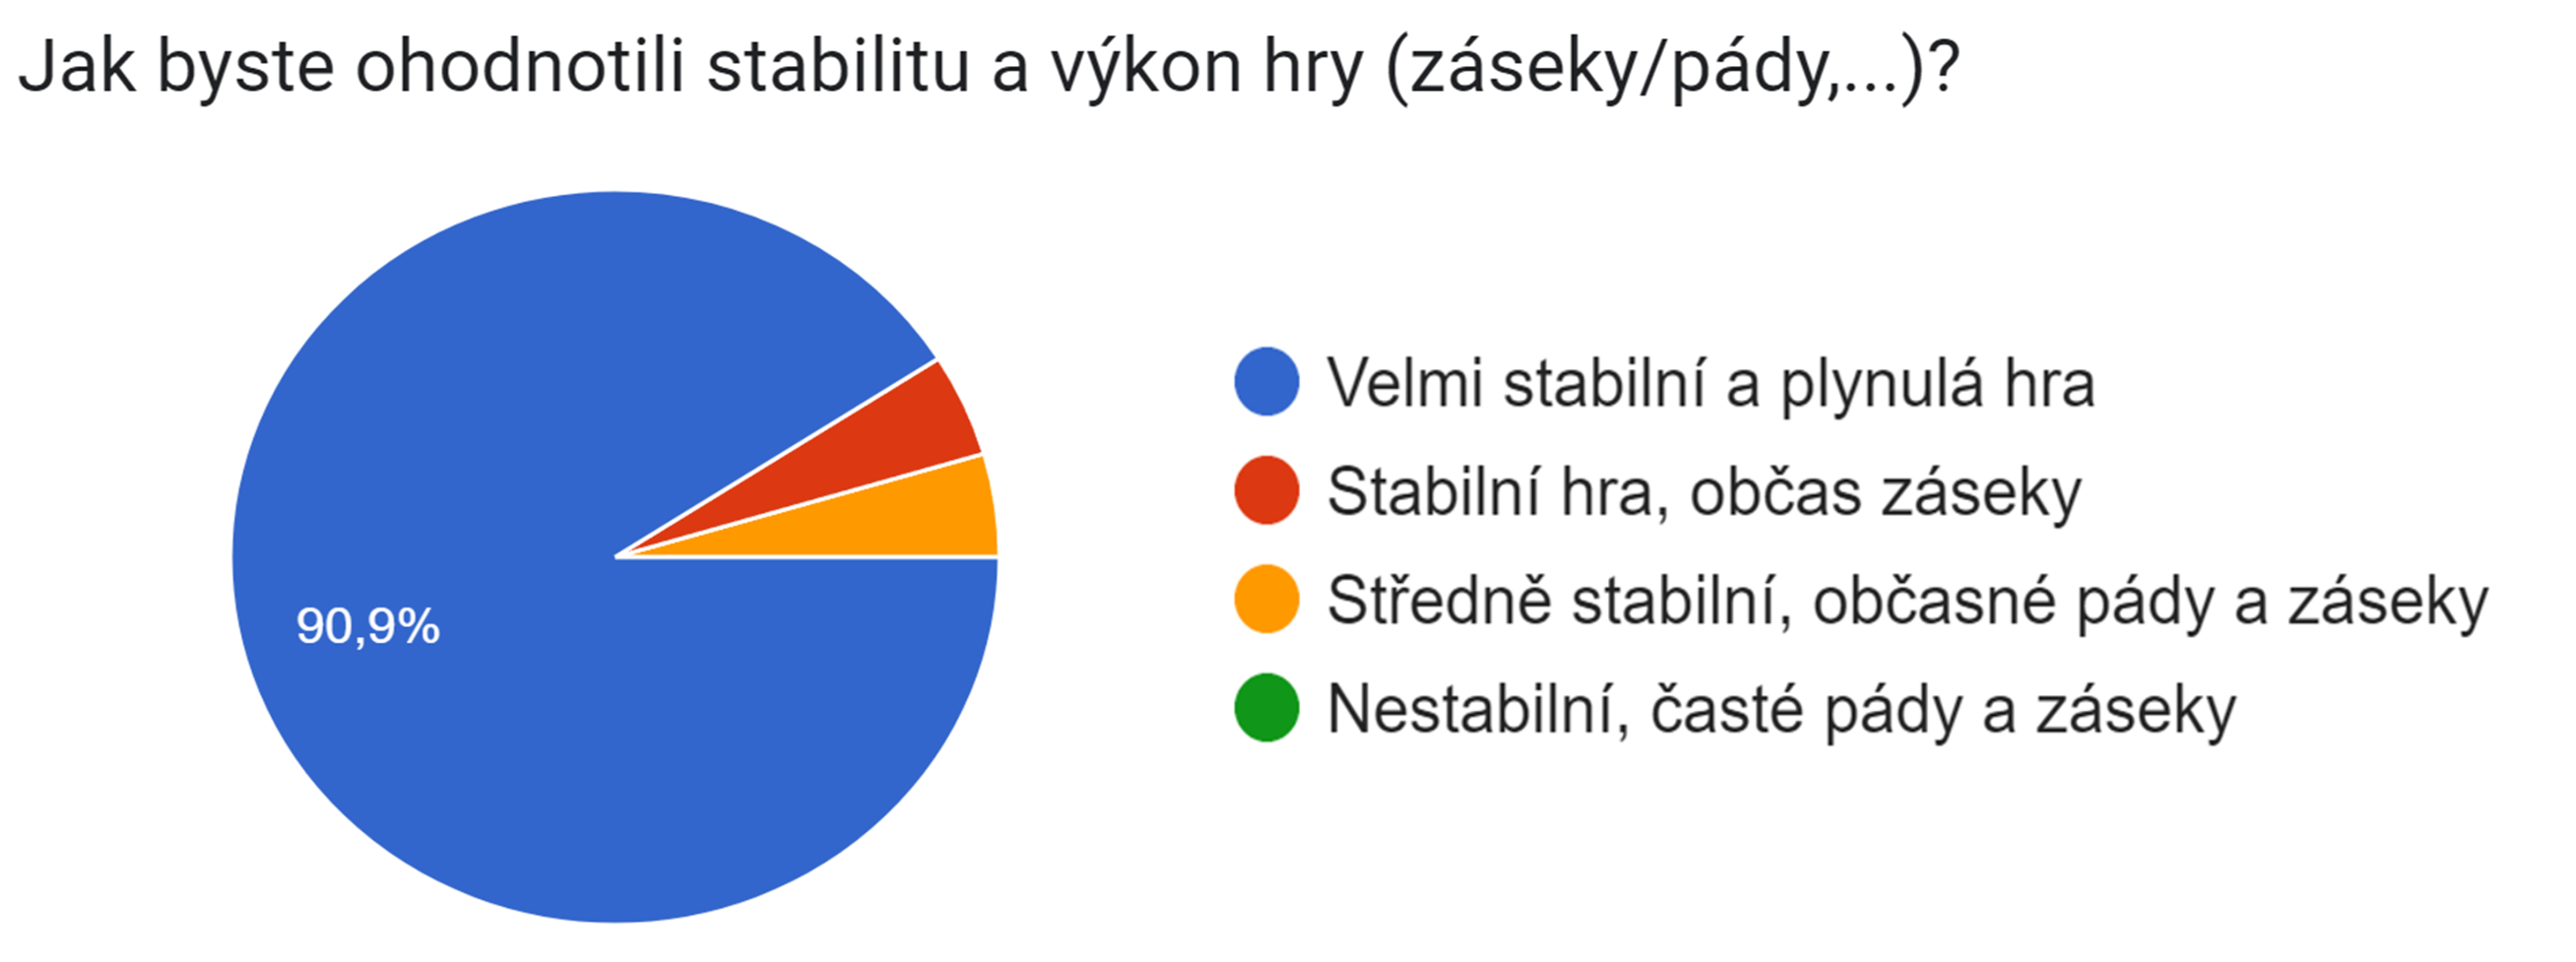
\includegraphics[width=0.85\textwidth]{obrazky-figures/ch5/hodnoceni_stabilita.png}
    \caption{Graf odpovědí na otázku \uv{Jak byste ohodnotili stabilitu a výkon hry (záseky/pády,...)?}.}
    \label{fig:hodnoceni_stabilita}
\end{figure}

\subsection*{Náročnost}
Na náročnost hry a její postupné zvyšování obtížností úrovně byl převážně kladný názor, i~když se našli někteří (3 testeři) kteří nepocítili rozdíly mezi různými úrovněmi. Někteří si naopak přáli možnost lehčího vyhýbání se nepřátelům, jelikož boje byly moc složité a bylo na ně málo místa. Také ale přišlo pár žádostí na zlehčení bloudění, a to například přidáním odhalující se minimapy, předmětu na poznačování cest, či seznamu hledaných předmětů a~nepřátel na začátku úrovně. Pár hráčům přišlo, že se nepřátelé a předměty neobjevují nějak kontrolovaně, například že v některých úrovních se jim nepovedlo potkat žádného nepřítele a v jiných i několik, podobné reakce byly i u předmětů a jeden tester dokonce oznámil, že se mu v jedné úrovni nedařilo najít konec hry (portál). 

Na základě zpětné vazby ohledně obtížnosti hry bylo nutné přemýšlet nad úpravou některých herních objektů. Jedním z nich byly boty/předmět na zrychlení, které poskytovaly hráči velké zrychlení po omezenou dobu. Další stížnosti se týkaly nepřítele \uv{slime}, který byl příliš obtížný kvůli svému excesivnímu zpomalení hráče. Také byly identifikovány problémy s nepřítelem "boar"/divočák, který se zasekával na hráčské postavě kvůli svému speciálnímu útoku a často zůstával uvízlý na zdech, což snižovalo jeho herní výzvu.

\begin{figure}[H]
    \centering
    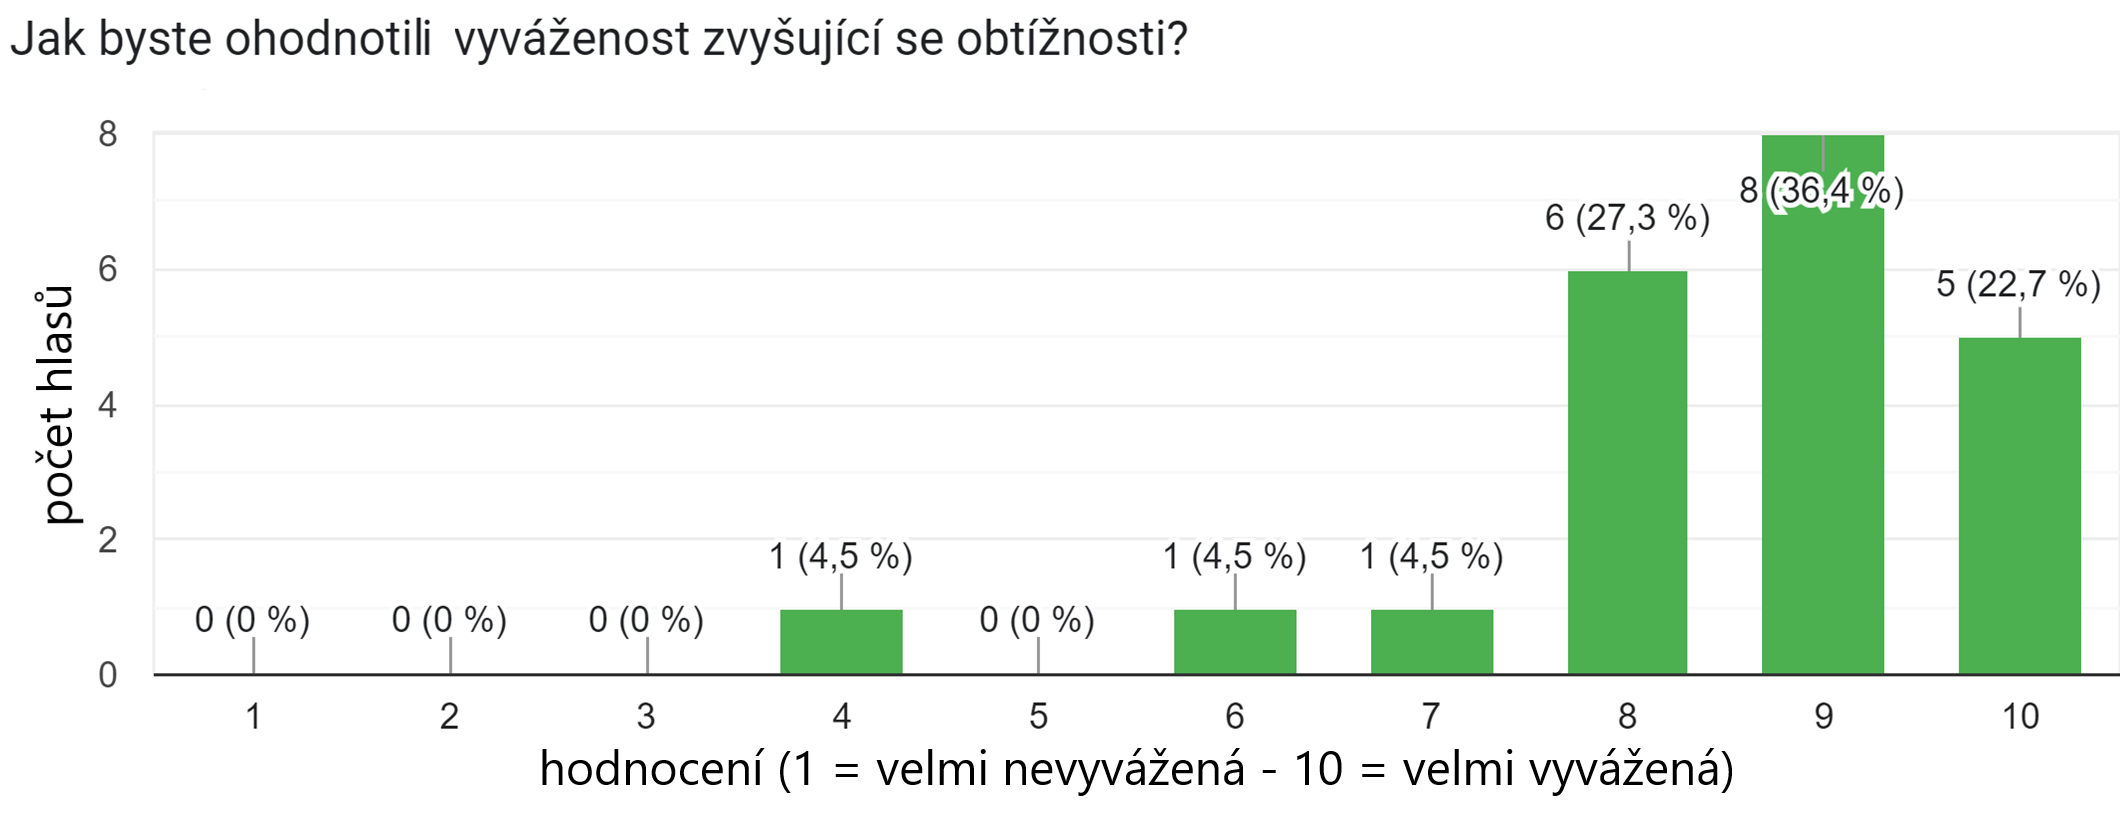
\includegraphics[width=\textwidth, height=0.25\textheight]{obrazky-figures/ch5/hodnoceni_vyvazenost.png}
    \caption{Graf odpovědí na otázku \uv{Jak byste ohodnotili vyváženost zvyšující se obtížnosti?}.}
    \label{fig:hodnoceni_vyvazenost}
\end{figure}

%--------------------------
% Závěr testování
\section{Závěr testování}
\subsection*{Implementované změny}
Na základě dotazníku byla vyhodnocena zpětná vazba, včetně otázky číslo 9 \uv{Jaké další funkce/vlastnosti/prvky byste ve hře ocenili/změnili?}, návrhy a poznámky byly rozděleny na skupiny \uv{implementované} a \uv{zavrhnuté a pro budoucí práci} a to v závislosti na jejich důležitosti pro hratelnost/vyváženost/chod hry, složitosti implementace a dle počtu žádostí o změnu/přidání.

\subsubsection*{\textbullet Hratelnost}
Hlavním problémem, který vyžadoval opravu, jak je již zmíněno v kapitole~\ref{chap:Analýza výsledků} Analýza výsledků, bylo počítání skóre. Proto byla vytvořena nová rovnice~\todo{viz rovnice x.x} na počítání skóre a do kódu byla přidaná kontrola zajišťující, že výsledné skóre z úrovně nemůže být nižší než 0. Také byl pro řazení skóre implementován lehčí a spolehlivější bubble sort namísto nativního Godot řazení.

Druhý častý problém testerů byl s nepochopením významu některých předmětů, a tedy i absence legendy/průvodce herními objekty. Proto byla přidaná do menu záložka \uv{Guide}, neboli \uv{Průvodce}, jenž má 4 stránky. První stránka \uv{Basics}, vysvětluje hráči základní ovládání, prioritu úkolů pro získání nejvyššího skóre a připomíná hráči mortalitu jeho herní postavy v závislosti na ikonách srdíček v levé části obrazovky. Další část \uv{Enemies} popisuje všechny nepřátele ve hře, jejich životy a speciální vlastnosti. Vlastnosti předmětů a~pastí/překážek pak popisují stránky \uv{Items} a \uv{Traps}.

Následně bylo potřeba upravit pohled kamery, aby se vyvarovalo problémům s postavičkou opouštějící střed obrazovky a způsobující nečekané kolize. Řešením bylo zvýšení rychlosti posunu kamery (na 16 pixelů, velikost 1 dlaždice hry) a důkladnější vycentrování postavy, rozdíl mezi původní kamerou a novou je vidět na obrázku~\ref{fig:rozdil_kamer}.

Hráčská postava prošla také aktualizací, jelikož její diagonální pohyb je v aktualizované formě stejně rychlý jak pohyb vertikální/horizontální, čehož bylo docíleno pomocí normalizace rychlostního vektoru. Také byl upraven čas vyslání signálu útoku hráče na nepřítele, aby byl synchronizovaný s animací útoku (čas kdy hráčská postava sekne zbraní, oproti původnímu napřahování se).

\begin{figure}[hb]
    \centering
    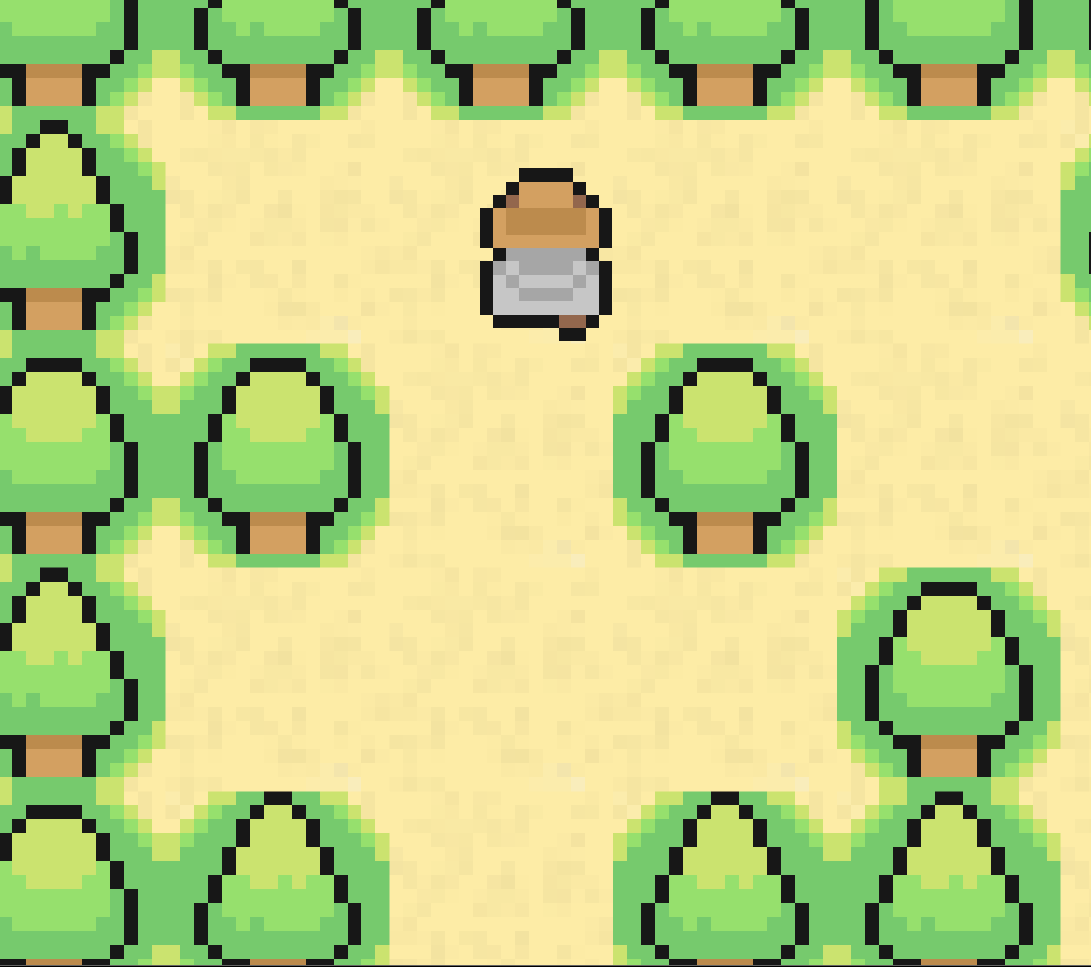
\includegraphics[width=0.45\textwidth]{obrazky-figures/ch5/old_camera.png}\hspace{0.5cm}
    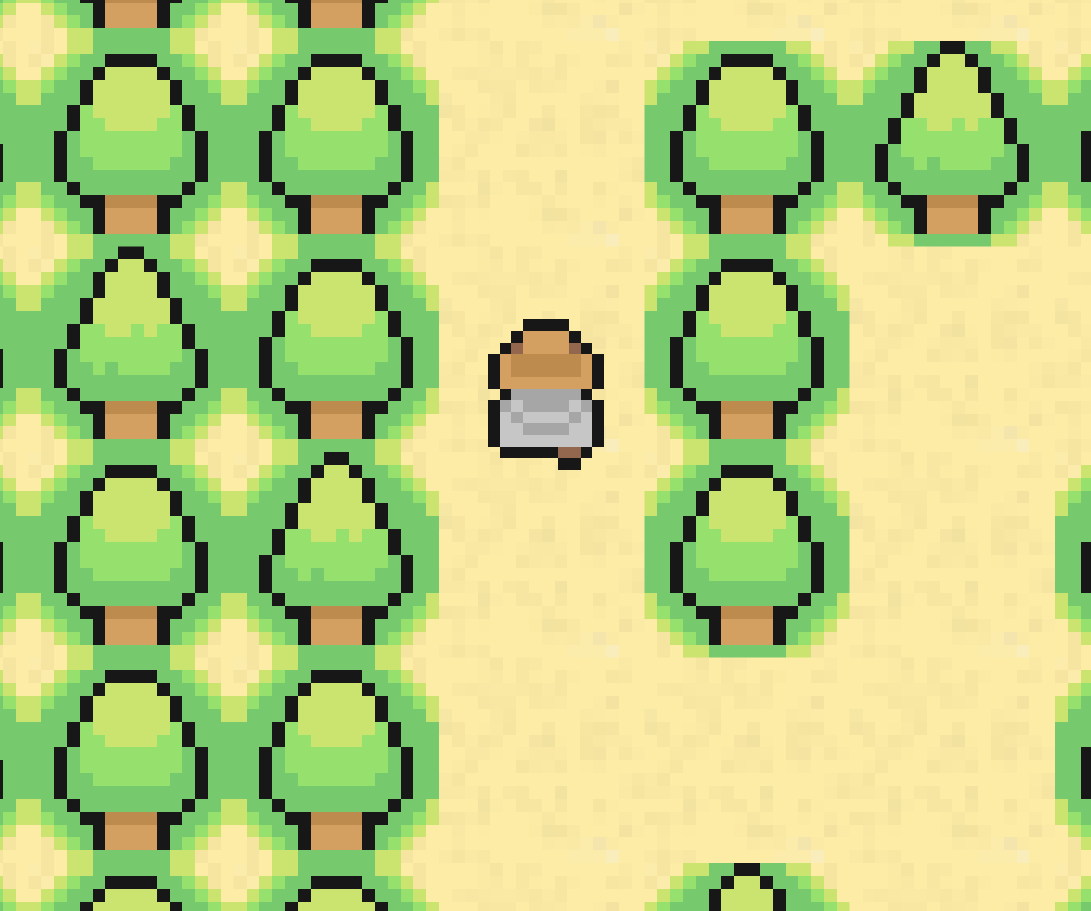
\includegraphics[width=0.474\textwidth]{obrazky-figures/ch5/new_camera.png}
    \caption{Rozdíl mezi pohledem staré kamery (vlevo) a nové (vpravo).}
    \label{fig:rozdil_kamer}
\end{figure}


\begin{figure}[ht]
    \centering
    
\includegraphics[width=0.1\textwidth]{obrazky-figures/ch5/new_demage.png}\hspace{3cm}
    
\includegraphics[width=0.1\textwidth]{obrazky-figures/ch5/new_speed.png}
    \caption{Nové, vylepšené ikony zvýšení poškození a zrychlení.}
    \label{fig:new_icons}
\end{figure}

\subsubsection*{\textbullet Uživatelské rozhraní a grafická stránka hry}
Z ohledu uživatelského rozhraní bylo na žádost testerů přidáno viditelné počítaní času stráveného na úrovní v horní liště hry. Je to kompromis, jelikož kvůli způsobu počítaní skóre (tedy odečítání uplynulého času) by bylo ubývající skóre pro hráče matoucí. V liště byl i zvětšen text popisků informačních sloupců (\uv{HP} a \uv{MODS}) pro zdůraznění jejich důležitosti.

Významnou změnou pro UI je přidání několika setinového zamrznutí ovládání po vstupu do obrazovky shrnující úspěšné dokončení úrovně. K tomu bylo přidána vyskakující okna potvrzující hráčovo rozhodnutí o opuštění hry, či navrácení se ze hry do menu. Tyto změny byly mířené na testery, kteří měli problém s mylným vypínáním hry. Pro hráčské pohodlí je hra spouštěna namísto předvolby celé obrazovky pouze v maximalizovaném okně. Také hráčům bylo umožněno odejít z pauzy pomocí žádaného tlačítka \textit{Esc}. Dále byla poupravena textura zvolených tlačítek, a to pomocí přidání světlého rámečku ohraničující vybrané tlačítko.
Ikony vylepšení v sloupci \uv{MODS} prošly grafickou úpravou. Při sbírání mečů se nyní zobrazuje ikona meče, nově s rámečkem, vyjadřujícím poškození. Podobně byla upravena ikona bot pro zrychlení, která nově zobrazuje násobek původní rychlosti. Obě nové ikony jsou vidět na obrázku~\ref{fig:new_icons}. Byla také přidána animace přičtení skóre při sebrání truhly pro vizuální vysvětlení jejího významu. Textura pasti byla opravena a již nezobrazuje kus jiné textury.

\subsubsection*{\textbullet Stabilita programu}
Jak již bylo zmíněno v analýze dotazníku, při dodatečném testování nebylo možné zreplikovat pád hry, jenž jeden z testerů popisoval. I tak ale byla přidána ikona potvrzení jména po stisknutí klávesy \textit{Enter} na obrazovce konce hry, která má naznačovat uživateli úspěšné dokončení uložení výsledků hry. Vzhledem k spokojenosti ostatních testerů se stabilitou hry nebylo třeba implementovat žádné úpravy zajišťující lepší stabilitu.

\subsubsection*{\textbullet Náročnost}
Vzhledem k několika feedbackům o nesprávném generování, kdy chyběly v některých úrovních nepřátelé, předměty a či portál/cíl hry, bylo provedeno důkladné testování na mnoha úrovních testujících, zda algoritmy generování odpovídají očekávaní. Nebyly nalezeny žádné nesrovnalosti s návrhem, vše se generuje podle očekávání a ve správných počtech.

Na základě zpětné vazby byla upravena celková náročnost hry. Jelikož pár hráčům přišlo, že se obtížnost zvyšuje moc pomalu, byla snížena úroveň, na které se poprvé objeví nepřítel na úroveň 3. Naopak ale byla zvýšena výzva pro možnost procházení bludiště bez bojů díky zmenšení nepřátelských modelů a snížení vzdálenosti od které začnou pronásledovat hráče na 3 bloky. Na vyvážení této změny byla zvýšena bodoví odměna za zabití nepřítele. Díky tomu má hráč stále motivaci s nepříteli radši bojovat než se jim vyhýbat.

Byl přepracován předmět lektvar zrychlení, který nyní poskytuje dlouhodobé mírné zrychlení hráče, na rozdíl od původního krátkodobého rapidního zrychlení. Úpravu dostal i \uv{slime} (zpomalovací nepřítel) jehož zpomalení se již nenásobí, ale pouze obnovuje časovač zpomalení a jeho zdraví bylo sníženo z 10 na 8. Nakonec byl odstraněn nepřítel \uv{boar}/divočák, který byl na základě dodatečného testování a snah o opravu vyhodnocen jako nevhodný do prostorů bludiště.

\subsection*{Zavrhnuté návrhy a návrhy pro budoucí práci}
Ve zpětné vazbě bylo získáno mnoho návrhů na úpravu hry. Některé z nich byly bohužel komplexní a vzhledem k období, ve kterém se testování odehrávalo, již nebyl čas je implementovat. Jiné byly naopak vyhodnoceny jako nápady, které by podkopávali hlavní nápad hry, tedy bloudění a simulace reálného labyrintu.

\noindent Zavrhnuté nápady:
\begin{itemize}
    \item Zobrazení skóre ve hře\,--\,matoucí kvůli způsobu počítání skóre, nahrazeno zobrazením času.
    \item  Ukázka získatelných předmětů na začátku úrovně\,--\, nabádalo by k ignorování nepotřebných předmětů, čímž by byl ztracen důvod pro důkladné prohledávání bludiště.
    \item  Oddálení kamery\,--\,aktuální velikost ideální k udržení zmatení simulující bloudění.
    \item Zobrazení dokončené mapy bludiště\,--\,rušivé, bránící plynulému přechodu do další úrovně.
\end{itemize}

\noindent Návrhy pro budoucí práci:
\begin{itemize}
    \item Odhlovací minimapa\,--\,vhodná pro lehčí verzi bludiště/vyšší úrovně, v základní verzi by odebrala motiv simulace reálného bludiště.
    (návrh na obrázeku~\ref{fig:map_idea}).
    \item Hudba\,--\,není čas a přístup k vytvoření vlastní hudby.
    \item Obchod/Editace postavy za sesbírané skóre\,--\,podporuje opakované hraní hry kvůli získaní přizpůsobitelných předmětů.
    \item  Předmět na poznačování prošlých úseků\,--\,vhodný pro pozdější, větší, úrovně, možnost implementace jako sbíratelný předmět.
\end{itemize}

\begin{figure}[H]
    \centering
    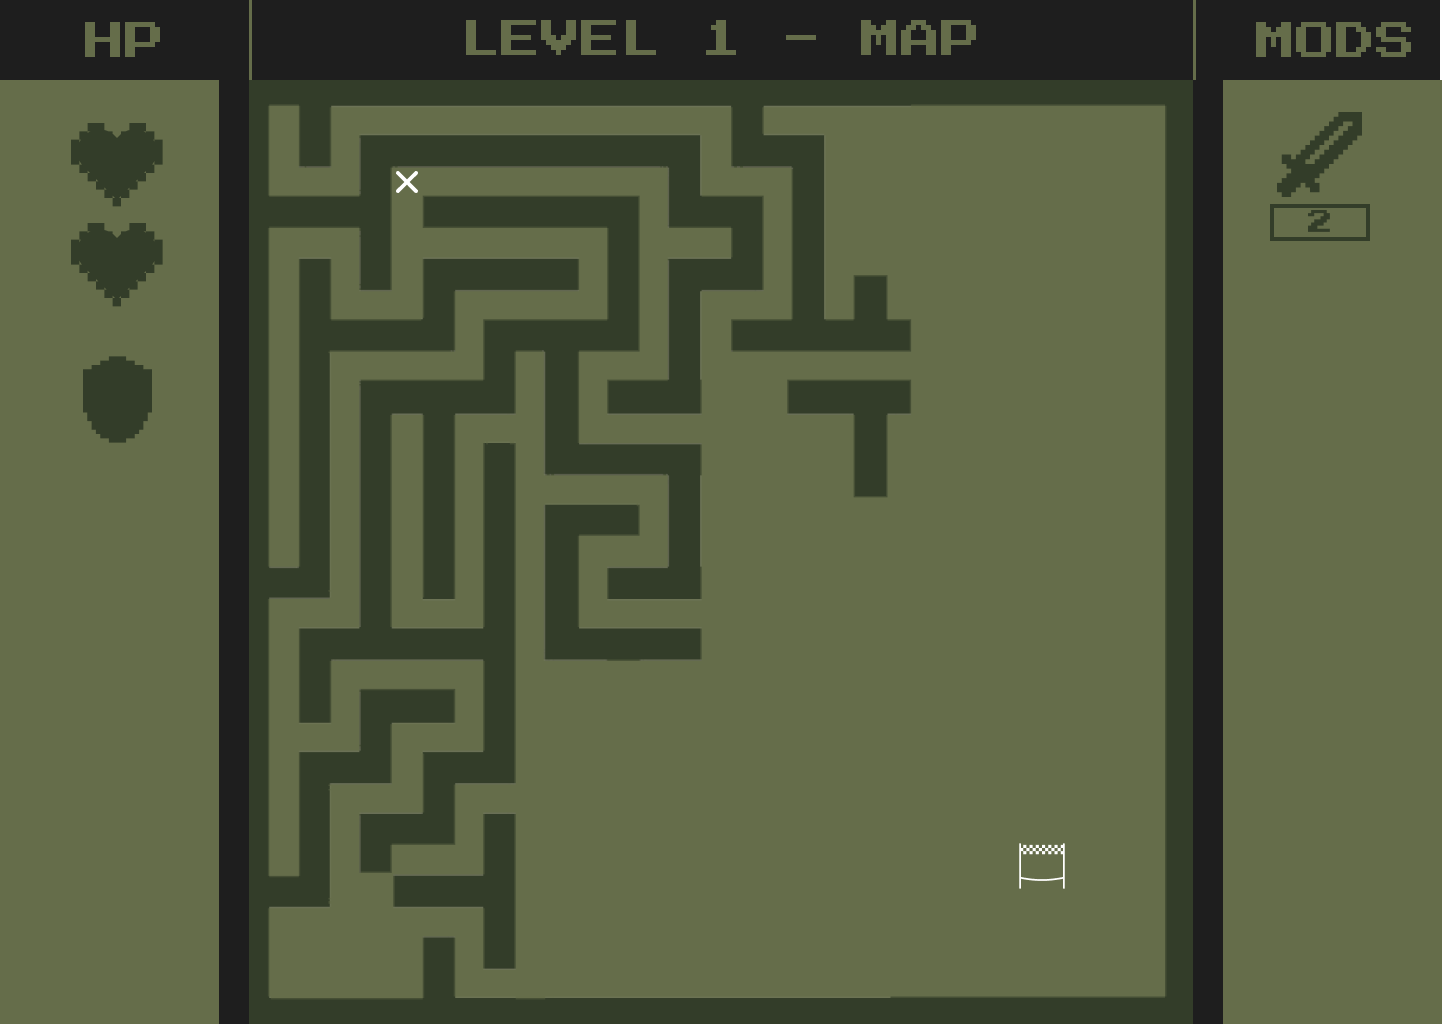
\includegraphics[width=0.55\textwidth, height=0.22\textheight]{obrazky-figures/ch5/Game_screen-MAP.png}
    \caption{Možný návrh odkrývající se mapy hry ve Figma.}
    \label{fig:map_idea}
\end{figure}

%===---------------====
% ZAVER
%===---------------====
\chapter{Závěr}
\todo{Dopsat - az na konci}
%===============================================================================

% Pro kompilaci po částech (viz projekt.tex) nutno odkomentovat
%\end{document}

  \fi
  
  % Kompilace po částech (viz výše, nutno odkomentovat a zakomentovat input výše)
  % Compilation piecewise (see above, it is necessary to uncomment it and comment out input above)
  %\subfile{chapters/projekt-01-uvod-introduction}
  % ...
  %\subfile{chapters/projekt-05-zaver-conclusion}

  % Pouzita literatura / Bibliography
  % ----------------------------------------------
\ifslovak
  \makeatletter
  \def\@openbib@code{\addcontentsline{toc}{chapter}{Literatúra}}
  \makeatother
  \bibliographystyle{bib-styles/Pysny/skplain}
\else
  \ifczech
    \makeatletter
    \def\@openbib@code{\addcontentsline{toc}{chapter}{Literatura}}
    \makeatother
    \bibliographystyle{bib-styles/Pysny/czplain}
  \else 
    \makeatletter
    \def\@openbib@code{\addcontentsline{toc}{chapter}{Bibliography}}
    \makeatother
    \bibliographystyle{bib-styles/Pysny/enplain}
  %  \bibliographystyle{alpha}
  \fi
\fi
  \begin{flushleft}
  \bibliography{projekt-20-literatura-bibliography}
  \end{flushleft}

  % vynechani stranky v oboustrannem rezimu
  % Skip the page in the two-sided mode
  \iftwoside
    \cleardoublepage
  \fi

  % Prilohy / Appendices
  % ---------------------------------------------
  \appendix
\ifczech
  \renewcommand{\appendixpagename}{Přílohy}
  \renewcommand{\appendixtocname}{Přílohy}
  \renewcommand{\appendixname}{Příloha}
\fi
\ifslovak
  \renewcommand{\appendixpagename}{Prílohy}
  \renewcommand{\appendixtocname}{Prílohy}
  \renewcommand{\appendixname}{Príloha}
\fi
%  \appendixpage

% vynechani stranky v oboustrannem rezimu
% Skip the page in the two-sided mode
%\iftwoside
%  \cleardoublepage
%\fi
  
\ifslovak
%  \section*{Zoznam príloh}
%  \addcontentsline{toc}{section}{Zoznam príloh}
\else
  \ifczech
%    \section*{Seznam příloh}
%    \addcontentsline{toc}{section}{Seznam příloh}
  \else
%    \section*{List of Appendices}
%    \addcontentsline{toc}{section}{List of Appendices}
  \fi
\fi
  \startcontents[chapters]
  \setlength{\parskip}{0pt} 
  % seznam příloh / list of appendices
  % \printcontents[chapters]{l}{0}{\setcounter{tocdepth}{2}}
  
  \ifODSAZ
    \setlength{\parskip}{0.5\bigskipamount}
  \else
    \setlength{\parskip}{0pt}
  \fi
  
  % vynechani stranky v oboustrannem rezimu
  \iftwoside
    \cleardoublepage
  \fi
  
  % Přílohy / Appendices
  \ifenglish
    \input{projekt-30-prilohy-appendices-en}
  \else
    % Tento soubor nahraďte vlastním souborem s přílohami (nadpisy níže jsou pouze pro příklad)

% Pro kompilaci po částech (viz projekt.tex), nutno odkomentovat a upravit
%\documentclass[../projekt.tex]{subfiles}
%\begin{document}

% Umístění obsahu paměťového média do příloh je vhodné konzultovat s vedoucím
%\chapter{Obsah přiloženého paměťového média}

%\chapter{Manuál}

%\chapter{Konfigurační soubor}

%\chapter{RelaxNG Schéma konfiguračního souboru}

%\chapter{Plakát}

\chapter{Struktura odevzdaného adresáře}\label{chap:file_directory}
\todo{txt s game assety}

\chapter{Výsledky experimentů s mapou}\label{chap:map_experiments}

\chapter{Výsledky uživatelského testování}\label{chap:user_testing}

\begin{table}[htbp]
\centering
\begin{tabularx}{\textwidth}{|X|X|X|}
\hline
\multicolumn{1}{|c|}{\textbf{otázka č. 1}} & \multicolumn{1}{c|}{\textbf{otázka č. 2}} & \multicolumn{1}{c|}{\textbf{otázka č. 3}} \\ \hline
\textbf{Kolik času jste strávili u hraní?} & \textbf{Jaká byla vaše nejvyšší dosažená úroveň (level)?} & \textbf{Jaký je váš celkový dojem ze hry?} (1 = velmi negativní - 10 = velmi pozitivní) \\ \hline
0:03:50 & 7 & 8 \\ \hline
0:07:00 & 12 & 7 \\ \hline
0:10:00 & 11 & 5 \\ \hline
0:10:55 & 9 & 8 \\ \hline
0:12:00 & 11 & 8 \\ \hline
0:23:00 & 10 & 8 \\ \hline
0:20:00 & 16 & 8 \\ \hline
0:20:00 & 8 & 9 \\ \hline
1:10:25 & 20 & 10 \\ \hline
0:20:00 & 11 & 9 \\ \hline
1:40:00 & 28 & 8 \\ \hline
0:30:00 & 20 & 7 \\ \hline
0:50:00 & 18 & 9 \\ \hline
0:30:00 & 11 & 5 \\ \hline
0:20:00 & 12 & 9 \\ \hline
0:20:00 & 6 & 9 \\ \hline
0:15:00 & 9 & 7 \\ \hline
0:15:00 & 15 & 10 \\ \hline
0:12:00 & 19 & 8 \\ \hline
0:40:00 & 22 & 7 \\ \hline
1:00:00 & 10 & 10 \\ \hline
0:58:25 & 15 & 9 \\ \hline
\end{tabularx}
\caption{1. část výsledků uživatelského hodnocení\,--\,obecné otázky ohledně hratelnosti.}
\end{table}

\begin{table}[htbp]
\centering
\begin{tabularx}{\textwidth}{|X|X|}
\hline
\multicolumn{1}{|c|}{\textbf{otázka č. 4}} & \multicolumn{1}{c|}{\textbf{otázka č. 5}} \\ \hline
\textbf{Jak byste ohodnotili uživatelské rozhraní a celkovou přehlednost hry?} (1 = velmi nepřehledné - 10 = velmi přehledné) & \textbf{Jak byste ohodnotili stabilitu a výkon hry (záseky/pády,...)?} \\ \hline
9 & Velmi stabilní a plynulá hra \\ \hline
9 & Velmi stabilní a plynulá hra \\ \hline
5 & Velmi stabilní a plynulá hra \\ \hline
8 & Velmi stabilní a plynulá hra \\ \hline
10 & Velmi stabilní a plynulá hra \\ \hline
10 & Velmi stabilní a plynulá hra \\ \hline
9 & Velmi stabilní a plynulá hra \\ \hline
10 & Velmi stabilní a plynulá hra \\ \hline
1 & Velmi stabilní a plynulá hra \\ \hline
8 & Velmi stabilní a plynulá hra \\ \hline
8 & Velmi stabilní a plynulá hra \\ \hline
8 & Velmi stabilní a plynulá hra \\ \hline
9 & Velmi stabilní a plynulá hra \\ \hline
7 & Středně stabilní, občasné pády a záseky \\ \hline
7 & Velmi stabilní a plynulá hra \\ \hline
7 & Velmi stabilní a plynulá hra \\ \hline
8 & Velmi stabilní a plynulá hra \\ \hline
10 & Velmi stabilní a plynulá hra \\ \hline
10 & Velmi stabilní a plynulá hra \\ \hline
4 & Stabilní hra, občas záseky \\ \hline
10 & Velmi stabilní a plynulá hra \\ \hline
9 & Velmi stabilní a plynulá hra \\ \hline
\end{tabularx}
\caption{2. část výsledků uživatelského hodnocení\,--\,Uživatelské rozhraní a stabilita}
\end{table}

\begin{table}[htbp]
\centering
\begin{tabularx}{\textwidth}{|X|X|X|}
\hline
\multicolumn{1}{|c|}{\textbf{otázka č. 6}} & \multicolumn{1}{c|}{\textbf{otázka č. 7}} & \multicolumn{1}{c|}{\textbf{otázka č. 8}} \\ \hline
\textbf{Co pro vás bylo nejtěžší?} & \textbf{Jak byste ohodnotil vyváženost zvyšující se obtížnosti?} & \textbf{Pokud jste hodnotili hru jako spíše nevyváženou, jaký k tomu byl důvod?} \\ \hline
Nepřátelé & 9 & \\ \hline
Nepřátelé & 9 & \\ \hline
Nepřátelé & 10 & \\ \hline
Nepřátelé & 8 & \\ \hline
Orientace v bludišti & 8 & \\ \hline
Orientace v bludišti & 9 & Ve vyšších levelech se mi spíše odečítaly body než přičítaly \\ \hline
Rychlost projití levelu & 9 & \\ \hline
Orientace v bludišti & 7 & Vlastně mi to přišlo fajn, ale ke konci už jsem bloudil opravdu dlouho v těch bludištích, takže už mě to ani nebavilo :( \\ \hline
Když člověk vleze do exitu z hora/dola a drží klávesu, tak se v menu trefí na exit hry. & 8 & U některých běhů nebyly skoro žádné předměty, u jiných jich bylo moc. \\ \hline
Orientace v bludišti & 4 & Nepocítila jsem rozdíly mezi jednotlivými úrovněmi, např. 1 a 3, 5 a 10. Nebyla tam jasná změna v obtížnosti, někdy stoupala příliš pomalu. \\ \hline
Orientace v bludišti & 9 & Všechno bylo vyvážené, dokud se tam neobjevil lučišník. \\ \hline
Orientace v bludišti & 10 & \\ \hline
Nepřátelé & 6 & Celková obtížnost se zvyšuje moc pomalu \\ \hline
Nepřátelé & 9 & \\ \hline
Nepřátelé & 10 & \\ \hline
Nepřátelé & 9 & \\ \hline
Nepřátelé & 8 & \\ \hline
Nepřátelé & 10 & \\ \hline
Nepřátelé & 8 & Celková obtížnost se zvyšuje moc pomalu \\ \hline
Orientace v bludišti & 8 & \\ \hline
Nepřátelé & 9 & \\ \hline
Nepřátelé & 10 & \\ \hline
\end{tabularx}
\caption{3. část výsledků uživatelského hodnocení\,--\,Náročnost a vyváženost}
\end{table}

\begin{table}[htbp]
\centering
\begin{tabularx}{\textwidth}{|X|X|X|}
\hline
\multicolumn{1}{|c|}{\textbf{otázka č. 9}} \\ \hline
\textbf{Jaké další funkce/vlastnosti/prvky byste ve hře ocenili/změnili?} \\ \hline

Legenda co dělají jednotlivé itemy a nepřátelé, vysvětlení jak se počítá skóre \\ \hline 

Opětovné sbírání mečů nemá nejspíše žádný další účinek na hraní. Což takhle \uv{stackovat} nebo zvyšovat damage? Předmět co zvyšuje rychlost by mohl vydržet déle než jenom těch cca 5 vteřin. \\ \hline

1. Na začiatku levelu by bolo dobré ukázať aké predmety je možné v tomto levely získať. \\ 
2. Odhalovacia minimapa.\\ 
3. Skóre počas levelu. Ja som dokonca získal záporné skóre. \\ \hline

Jen drobnost, ale pokud dojde k odečtení skóre, bylo by lepší skóre odečíst rovnou a nedávat +    -score. Bavím se nyní o obrazovce, která se zobrazí po dokončení levelu.\\ \hline

Celkovy cas straveny ve hre v danem levelu nebo v celkovem, lepsi viditelnosti zvoleneho pole v menu i pri death screen\\ \hline

Libí se mi variabilita nepřátel a bludišť, byla by fajn nějaká hudba, super by bylo si za body kustomizovat panáčka (čepičky a tak), hra mě fakt bavila, určitě ji budu hrát i dál \\ \hline

Změnil bych to, že při posunu nahoru je menší zorné pole než dolů.\\ \hline

ocenil bych kdyby šlo hru odpauznout klávesou escape, jo a btw, dvakrát během hraní se mi zapnul snipping tool (který obyčejně zapínám klávesou prtscr), možná (asi) je to nějaký issue u mě co se hrou nesouvisí, ale stalo se mi to dvakrát takže to je celkem sus, mám windows 11 23h2 build 22631.3374, ale jinak pecka moc se mi to líbí\\ \hline

Dobrá hra, pár věcí: Lze útočit přes rohy (pravý horní roh). Elixir zrychlení maže druhý elixir zrychlení. Ovládání ze hry se probublává do menu a tím se hra velmi snadno nechtěně vypne. Skore se nezobrazuje ve hře. Skoré se divně řadí. Občas je vzhůru nohama. Občas se přičítá negativní skóre? Meče se nesčítají/neobjevují v inventáři ve vícero instancích. Zpomalovací MOB je příliš těžký. Šlo by dodat vícero volných prostor, kde by se lépe bojovalo, než jen koridory? Poznačování prošlých úseků - třeba pomocí nějakého předmětu, který postava položí na zem? Past má když jsou schované ostany po levé straně podivné černé proužky. Nešel by trošku oddálit pohled? Když se běží nahoru, je kamera skoro u kraje hrací plochy a člověk snadno naběhne na ostny... Když se běží, tak postavička vibruje...\\ \hline

Není mi úplně jasná funkce některých (ochranných) prvků, např. štítu nebo bot.\\ \hline

pouze bych Přidal bych hudbu, animaci stromů(jak se hýbají ve větru) a nějaké \uv{consumable items} (předměty, které můžete vzít a aktivovat stisknutím tlačítka). Jinak je to skvělá hra.\\ \hline

Veľmi ma frustrovalo, že naraz na obrazovke vidím iba malú časť bludiska a dieliky sú obrovské. Páčil sa mi pixel art :)\\ \hline

Nevím, k čemu je sbírání truhel, jinak pěkná hra.\\ \hline

nepratele blokujici hrace jsou otravni; mozna trochu vice zvyraznit HP - nebylo mi jasne, jestli se jedna o zivoty co mam, nebo co muzu jeste doplnit + mi prijde, ze jsem tento placement neocekavala a dlouho jsem si jich vubec nevsimla - i s tim by vybarveni napr. na cerveno pomohlo\\ 
Ad. otazka pady - po dohrani a zadani jmena (bez diakritiky) a zmacknuti enteru hra spadla, po spusteni ale vse bylo ulozeno, to tak ciste pro info\\ 
Posledni poznamka: velke + za vizual, je to fakt pekny\\ \hline

\end{tabularx}
\caption{4. část výsledků uživatelského hodnocení\,--\,Návrhy testerů, část 1}
\end{table}


\begin{table}[htbp]
\centering
\begin{tabularx}{\textwidth}{|X|X|X|}
\hline
\multicolumn{1}{|c|}{\textbf{otázka č. 9}} \\ \hline
\textbf{Jaké další funkce/vlastnosti/prvky byste ve hře ocenili/změnili?} \\ \hline

maly vyhled je frustrujici, obzvlast v kombinaci s kolizemi s neprateli\\ \hline

- keď sa hráč pohybuje diagonálne, ide o dosť rýchlejšie\\ 
- nejaký zvuk by bol fajn, ale chápem, že to je iba alpha\\ 
- podľa animácie útoku som usúdil, že damage to dáva až ku koncu, ale potom som zistil, že ho dáva na začiatku\\ 
- tiles sú veľmi veľké\\ 
- páči sa mi ako hra vyzerá, má peknú farebnú paletu\\ 
- bigfoot ma zavrel snehuliakom do rohu a tam ma pomaly zabil, desivý týpek\\ \hline

Zrušil bych fullscreen po zapnutí, protože kvůli této \uv{feature} jsem nemohl přemístit hru na velkou obrazovku, musel jsem přesouvat video, které jsem měl puštěné do pozadí naopak na druhou obrazovku, což bylo zbytečně komplikované, protože hra byla ve fullscreenu nad videem.\\ 
Nepřátelům se obvykle nedá vyhnout kvůli úzkým koridorům, ocenil bych aby bylo reálně možné se jim vyhýbat.\\ 
Zpomalení od slima je otravně velké, snížil bych ho.\\ 
Záporný počet bodů za relativně rychle projitý level (oproti několika předchozím kde jsem byl pomalejší) mě celkem zarazil, zamyslel bych se nad způsobem výpočtu bodů.\\ 
Chybí vysvětlení že je možné nějak útočit.\\ 
Po skončení levelu se snadno překlikne v důsledku držení šipky ze hry na menu/vypnutí hry a dojde k nechtěnému vypnutí, ocenil bych otázku, zda si je volbou uživatel jistý nebo jinou formu, aby nedošlo k neúmyslnému vypnutí.\\ \hline

Hra se mi moc líbí, design je jednoduchý ale tak krásný, jednou chybu kterou jsem tam já osobně měla (mohla to být chyba v mojí nepozornosti), v jedné úrovni jsem nemohla najít portál do dalšího levelu a opravdu jsem to tam prošla celé, ale to je tak jediný negativní postřeh který jsem zaznamenala. Jinak ej to moc super! :-))\\ \hline

Rychlejší pohyb postavy skrz item bot \\ \hline

Přidání legendy nebo označení, co některé věci dělají. Například truhla by mohla mít nějaké zaznačení přidání bodů do skóre.\\ 
Přidání počitadla skóre do hry nejen při dokončení levelu.\\ 
Po sebrání meče se mod nepřidá - není jasné zda se poškození zvýší nebo že není možné mít více zbraní zároveň. \\ 
Útok divočáka skončil chybou, po zabití se divočák přichytil k hratelné postavě a po krátký časový interval v postavě byly zaseklé jeho ostatky.\\ 
Po ukončení hry a opětovném načtení hra vytvořila na levelu 21 mapu pro level 1.\\ \hline

někdy mi z truhličky nepadaly odměny, nevím jestli se jedná o bug nebo co by měla dělat, nepochopil jsem\\ \hline

Při hře mít  viditelné stopky, když se sebere meč podruhé - třeba nějaký upgrade, po skončení levelu by bylo hezké, kdyby se ukázala mapa daného labyrintu \\ \hline

\end{tabularx}
\caption{4. část výsledků uživatelského hodnocení\,--\,Návrhy testerů, část 2}
\end{table}


% Pro kompilaci po částech (viz projekt.tex) nutno odkomentovat
%\end{document}

  \fi
  
  % Kompilace po částech (viz výše, nutno odkomentovat)
  % Compilation piecewise (see above, it is necessary to uncomment it)
  %\subfile{projekt-30-prilohy-appendices}
  
\end{document}
